\documentclass{article}
\input{settings}

\begin{document}

%TITLE PAGE
\thispagestyle{empty}

\begin{center}
	\vfill
    \vspace*{0.3\textheight}

	\Huge
	\textbf{Analisi}
	
	\vspace{1cm}
	
	\Large
	\textit{Samuele Musiani}
	
	\vspace{3cm}
	
	\large
	September 19, 2022 - \today
	
    \normalsize
    
%	\vspace{0.33\textheight}
\end{center}

\tableofcontents
\hfill

\section{Introduzione agli appunti}

%Spiegare la natura degli appunti e il loro scopo. Definire docente e periodo di appunti. Non prendersi alcuna responsabilità su quanto sono giusti o sbagliati gli appunti. Libri di riferimento. La non rigorosità di molti argomenti.

\section{Insiemi}
\subsection{Simbologia}
Per indicare gli insiemi si utilizzano lettere maiuscole ($A, B, X, Y ...$). 
Per indicare gli elementi appartenenti ad un insieme si usano le lettere 
minuscole ($a, b, x, y ...$). Di seguito una lista di simboli necessari per 
lavorare con gli insiemi e la logica in generale:

\begin{multicols}{2}

\begin{itemize}
    \item $\in$ \qquad Appartiene
    \item $\notin$ \qquad Non appartiene
    \item $\forall$ \qquad Per ogni
    \item $:$ \textit{or} $|$ \qquad Tale che
    \item $\exists$ \qquad Esiste (almeno)
    \item $\nexists$ \qquad Non esiste
    \item $\exists \oc$ \qquad Esiste ed è unico
    
    \item $\subseteq$ \qquad Inclusione insiemi
    \item $\subsetneqq$ \qquad Inclusione stretta (cioè $A \subseteq B$ e $A 
        \neq B$)
    \item $\nsubseteq$ \qquad Non incluso
    
    \item $\cup$ \qquad Unione
    \item $\cap$ \qquad Intersezione
    \item $\emptyset$ \qquad Insieme vuoto
    \item $\setminus$ \qquad Meno tra insiemi
    \item $\mathbb{U}$ \qquad Insieme universale
    \item $\complement \left(A\right)$ \qquad Complementare di $A$ in 
        $\mathbb{U}$, cioè tutti gli elementi di $\mathbb{U}$ che non sono in 
        $A$ ($\complement \left(A\right) = \mathbb{U} \setminus A$).
    
    \item $\lor$ \qquad OR logico
    \item $\land$ \qquad AND logico
    \item $\implies$ \qquad Implica
    \item $\iff$ \qquad Coimplica, "se e solo se" 
\end{itemize}
\end{multicols}

\subsection{Proposizioni e utilizzo di simboli logici}

Le \textbf{proposizioni} sono "frasi" che hanno un valore di verità, cioè posso 
essere vere o false. Per legare due o più proposizioni si utilizzano svariati 
simboli logici. In generale la logica proposizionale si studia nel corso di 
logica quindi non ho intenzione di riportare più dello stretto necessario qui.

\begin{table}[H]
\centering
\begin{tabular}{|cc|c|c|c|}
    \hline
    p & q & \multicolumn{1}{l|}{p $\land$ q} & \multicolumn{1}{l|}{p $\lor$ q} 
        & \multicolumn{1}{l|}{p $\implies$ q} \\ \hline
    {\color[HTML]{000000} false} & {\color[HTML]{000000} false} & false & false 
        & true \\
    {\color[HTML]{000000} false} & {\color[HTML]{000000} true} & false & true 
        & true \\
    {\color[HTML]{000000} true} & {\color[HTML]{000000} false} & false & true 
        & false \\
    true & false & true & true & true \\ \hline
\end{tabular}

\caption{Tabella di verità per AND, OR e IMPLICAZIONE}
\end{table}

Nell'implicazione ($p \implies q$) $p$ è condizione sufficiente per $q$, mentre 
$q$ è condizione necessaria per $p$.

Se si vuole negare una proposizione si utilizza il simbolo di negazione ($^-$) 
oppure il classico $\neg$, quindi $p$ negato risulta $\overline{p}$ oppure 
$\neg p$. Di seguito alcune negazioni di simboli generali:
\begin{itemize}
    \item $\neg \forall = \exists$
    \item $\neg \exists = \forall$
\end{itemize}
Attenzione che i simboli $\not \exists$ e $\neq \exists$ hanno significati 
diversi. 

È interessante notare che se si ha un'implicazione, si negano entrambe le 
proposizioni e si scambiano i termini il risultato rimane invariato.

\begin{table}[H]
\centering
\begin{tabular}{|cc|c|c|}
\hline
    p & q & \multicolumn{1}{l|}{$p \implies q$} & \multicolumn{1}{l|}
    {$\overline{q} \implies \overline{p}$} \\ \hline
    {\color[HTML]{000000} false} & {\color[HTML]{000000} false} & false 
    & false \\
    {\color[HTML]{000000} false} & {\color[HTML]{000000} true} & false 
    & true \\
    {\color[HTML]{000000} true} & {\color[HTML]{000000} false} & false 
    & true \\
    true & false & true & true \\ \hline
\end{tabular}
\caption{Implicazione con termini negati e invertiti}
\end{table}

Avendo la stessa tabella di verità $p \implies q = \overline{q} \implies 
\overline{p}$. Da qui nasce la \textbf{dimostrazione per negazione} (o 
contronominale). Esempio: se vogliamo dimostrare che se $n^2$ \textit{è pari} 
allora $n$ \textit{è pari}, ci basta dimostrare che se $n$ \textit{è dispari} 
allora $n^2$ \textit{è dispari}:
\begin{equation*}
	n \; \text{dispari} \implies n^2 \; \text{dispari}
\end{equation*}
Assumiamo che $n$ sia dispari per dimostrare che $n^2$ è dispari. Per ipotesi:
\begin{equation*}
	\exists k \in \mathbb{N}: n = 2k + 1
\end{equation*}
Ne consegue che:
\begin{equation*}
	n^2 = (2k+1)^2 = 4k^2 + 4k + 1 = 2(2k^2 + 2k) + 1
\end{equation*}
Essendo $(2k^2 + 2k) \in \mathbb{N}$ ne consegue che:
\begin{equation*}
	2(2k^2 + 2k) + 1 \;\; \text{è dispari}
\end{equation*}
\hfill Qed.


\subsection{Insiemi numerici noti}

\subsubsection{Naturali, interi e razionali}

Il primo insieme che si introduce è l'insieme dei \textbf{numeri naturali}, 
indicato con $\mathbb{N}$. Non definiremo formalmente l'insieme, ci basti 
sapere che comprende tutti i numeri interi positivi. È generalmente scritto 
nella forma:
\begin{center}
    $\mathbb{N} = \{0, 1, 2, 3, ...\}$
\end{center}

Il secondo insieme che va introdotto è quello dei \textbf{numeri interi}. 
Questo insieme comprende tutti i numeri che non hanno la virgola (per l'appunto 
interi) e si distingue da $\mathbb{N}$ in quanto ha al suo interno anche i 
numeri negativi. Il suo simbolo è $\mathbb{Z}$ e viene generalmente scritto 
come segue:
\begin{center}
    $\mathbb{Z} = \{..., -2, -1, 0, 1, 2, ...\}$
\end{center}

Non sempre però è comodo descrivere gli insiemi elencando il loro termini (in 
realtà non viene quasi mai fatto in quanto si creerebbero delle ambiguità). È 
necessario quindi utilizzare una notazione diversa per descrivere un insieme, 
ed è quello che si usa anche per introdurre $\mathbb{Q}$, l'insieme dei 
\textbf{numeri razionali}:
\begin{center}
    \begin{equation*}
        \mathbb{Q} = \left\{\,\dfrac{p}{q}\, \middle| \, p, q \in \mathbb{Z},\, 
        q \neq 0 \right\}
    \end{equation*}
\end{center}
In questo caso l'insieme dei numeri razionali indica appunto l'insieme di tutte 
le frazioni\footnote{Matematici rigorosi abbiate pietà della mia anima}. E per 
esplicitarlo non cominciamo ad elencare tutte le frazioni, ma bensì utilizziamo 
una proposizione.

\subsubsection{Reali}
L'ultimo insieme che introduciamo è l'insieme dei \textbf{numeri reali}. Viene 
indicato con il simbolo $\mathbb{R}$ ed è l'insieme più importante di tutti i 
precedenti. Questo insieme viene introdotto perché all'insieme dei numeri 
razionali ($\mathbb{Q}$) mancano dei numeri.

Proviamo infatti a prendere una retta e a inserirci tutti i numeri che 
conosciamo per ora (cioè quelli contenuti in Q). Costruiamo ora un quadrato di 
lato 1, e proviamo a calcolare la lunghezza della sua diagonale con il teorema 
di Pitagora. Il numero che otterremo sarà $\sqrt{1^2+1^2} = \sqrt{2}$. Se 
proiettiamo questo numero sulla retta vediamo chiaramente che esiste un punto 
che corrisponde a $\sqrt{2}$.

\begin{figure}[h]
	\begin{center}

	\begin{tikzpicture}[scale=4]

		\draw[->] (0, 0) -- (2, 0);
		\draw[->] (0, 0) -- (0, 1.5);
		\draw[-] (1, 0) -- (1, 1);
		\draw[-] (0, 1) -- (1, 1);
		\draw[-] (0, 0) -- node[left, yshift=5pt] {$\sqrt{2}$} (1, 1);
			

		\draw (0,0) -- (1.414,0) arc(0:45:1.414);


		\draw[very thin, fill] (0,0) circle (0.4pt) node[left, yshift=10pt] 
            {$0$};
		\draw[very thin, fill] (1,0) circle (0.4pt) node[left, yshift=10pt] 
            {$1$};
		\draw[very thin, fill] (1.414,0) circle (0.4pt) node[right, 
            yshift=10pt] {$\sqrt{2}$};
	\end{tikzpicture}

	\end{center}
	\caption{$\sqrt{2}$ derivata dalla lunghezza della diagonale di un 
    quadrato}
\end{figure}


Questo punto è contenuto nell'insieme $\mathbb{Q}$? 

\pf{
	Dobbiamo provare che $\sqrt{2} \not \in \mathbb{Q}$. Assumiamo che sia 
    contenuto e riduciamoci a dimostrare l'assurdo. Se $\sqrt{2} \in 
    \mathbb{Q}$ significa che:
	\begin{equation*}
        \exists\, m, n, \in \mathbb{N} : \dfrac{m}{n} = \sqrt{2}
	\end{equation*}
	Cioè esistono due numeri appartenenti all'insieme dei numeri naturali tali 
    che il loro rapporto è esattamente $\sqrt{2}$. Ovviamente essendo una 
    frazione possiamo semplificare $m$ e $n$ fino ad eliminare tutti i loro 
    fattori comuni, cioè fino a farli diventare \textbf{coprimi} o meglio 
    $\mathrm{M.C.D}(m,n) = 1$.

	\begin{equation*}
        \dfrac{m}{n} = \sqrt{2} \implies \dfrac{m^2}{n^2} = \sqrt{2} 
        \implies m^2 = 2n^2
	\end{equation*}
	Possiamo quindi dedurre che $m^2$ è pari,  e quindi $m$ è pari\footnote{Lo 
    abbiamo visto qualche pagina sopra come esempio di dimostrazione per 
    negazione}.
	Quindi $\exists\, k \in \mathbb{N} : m = 2k$.
	\begin{equation*}
	m^2 = 2n^2 \implies (2k)^2 = 2n^2 \implies 4k^2 = 2n^2 \implies 2k^2 = n^2
	\end{equation*}
	Quindi se $n^2$ è pari, anche $n$ è pari.\\

	Abbiamo dimostrato che sia $m$ che $n$ sono pari, eppure avevamo imposto 
    che $m$ e $n$ non avessero fattori in comune. Assurdo! Quindi:
	\begin{equation*}
		\sqrt{2} \not \in \mathbb{Q}
	\end{equation*}

	\hfill Q.e.d.
}

Come abbiamo dimostrato $\sqrt{2}$ non appartiene all'insieme dei numeri 
razionali. Si può estendere quesa affermazione con il seguente teorema:
\thm{
    Sia $p \in \mathbb{N}$ un numero primo, allora $\sqrt{p} \not \in 
    \mathbb{Q}$
}
\pf{
    La dimostrazione è analoga al caso in cui $p = 2$. Si assume per assurdo 
    che:
    \begin{equation*}
        \exists m,n \in \mathbb{N} : \sqrt{p} = \dfrac{m}{n}
    \end{equation*}
    Assumiamo che $m$ e $n$ siano coprimi in quanto è sepre possibile 
    semplificare fino a farli diventare coprimi. In altre parole M.C.D$(m, n) 
    = 1$.
    Vale quindi che:
    \begin{equation*}
        p = \dfrac{m^2}{n^2} \implies n^2 \cdot p = m^2
    \end{equation*}
    Tutti i fattori di $m^2$ sono i fattori di $m$, quindi $p$ è un fattore di 
    $m$. $\exists k \in \mathbb{N}: m = kp$. Sostituende risulta:
    \begin{equation*}
        m^2 = p \cdot n^2 \implies (kp)^2 = p \cdot n^2 \implies k^2 \cdot 
        p^2 = p \cdot n^2 \implies k^2 \cdot p = n^2
    \end{equation*}
    Per la stessa osservazione fatta prima, questo significa che $p$ divide 
    $n$. Ma dividendo anche $m$ risulta che M.C.D$(m, n) = p$. Ed essendo $p$ 
    un numero primo $p \neq 1$. Assurdo! Quindi:
    \begin{equation*}
        \sqrt{p} \not \in \mathbb{Q}
    \end{equation*}

    \hfill Q.e.d.
}
Quindi tutti i numeri primi non appartengono all'insieme dei numeri razionali. 
Ma quanti numeri primi esistono?
\thm{
    I numeri primi sono infiniti
}
\pf{
    La dimostrazione è per assurdo quindi supponiamo che i numeri primi siano 
    finiti. Elenchiamoli in ordine crescente:
    \begin{equation*}
        p_1 < p_2 < p_3 < \cdots < p_n
    \end{equation*}
    Definiamo ora il numero: $m \vcentcolon = p_1 \cdot p_2 \cdots p_n + 1$. 
    Facciamo vedere che $m$ produce una contraddizione: $m > p_n$ quindi 
    essendo $p_n$ il massimo numero primo $m$ deve per forza essere non primo. 
    Essendo non primo $m$ deve per forza essere divisibile per almeno uno dei 
    numeri primi $p_1, p_2, \cdots, p_n$. Notiamo però che preso un qualsiasi 
    primo $p_i$, $m$ darà sempre resto $1$:
    \begin{equation*}
        m = p_i \cdot (p_1 \cdots p_{i - 1} \cdot p_{i + 1} \cdots p_n) + 1
    \end{equation*}
    Non essendo quindi divisibile per nessuno dei numeri primi $m$ deve per 
    forza essere primo, ma questo è assurdo in quanto $m$ non era primo per 
    l'osservazione fatta in precedenza.
    \hfill{Q.e.d.}
}

Ne consegue che esistono infiniti punti sulla retta che non appartengono a 
$\mathbb{Q}$, e anzi è molto più probabile che facendo la radice di un numero 
si ottenga un numero che non è incluso in $\mathbb{Q}$ piuttosto che il 
contrario. Quindi se si vuole formalizzare una teoria dei limiti è necessario 
lavorare su un insieme non "bucato", cioè un insieme \textbf{continuo}.
\bigbreak

La proprietà che infatti distingue e differenzia $\mathbb{R}$ da $\mathbb{Q}$ 
è proprio la continuità (non ci sono "buchi") e la completezza (tutti i punti 
sulla retta hanno associato un unico numero reale). Esiste infatti una 
\textbf{corrispondenza biunivoca} che associa tutti i punti della retta ai 
numeri reali.\footnote{Per approfondire il concetto di \textit{corrispondenza 
biunivoca} è necessario fare riferimento al capitolo legato alle funzioni.}
Per definire meglio la proprietà di completezza è necessario introdurre alcuni 
concetti:

\dfn{
    Dato $A \neq \emptyset$ e $A \subseteq R$
    \begin{enumerate}
        \item $M \in \mathbb{R}$ si dice \textbf{maggiorante} di $A$ se: 
            $\forall\, a \in A : a \leq M$.
        \item $m \in \mathbb{R}$ si dice \textbf{minorante} di $A$ se: 
            $\forall\, a \in A : m \leq a$.
        
        \item Se $A$ ammette un maggiorante è \textbf{superiormente limitato}.
        \item Se $A$ ammette un maggiorante è \textbf{inferiormente limitato}.
        \item Se $A$ ammettere un maggiorante e un minorante è 
            \textbf{limitato}.
        
        \item $b \in A$ si dice \textbf{massimo} di $A$ se $\forall\, a 
            \in A : a \leq b$.
        \item $c \in A$ si dice \textbf{minimo} di $A$ se $\forall\, a 
            \in A : c \leq a$.
        
        \item Il più piccolo dei maggioranti si chiama \textbf{estremo 
            superiore} di $A$. Si indicato con $\mathbf{sup}\,A$. Se il massimo 
            esiste coincide con l'estremo superiore. Se l'insieme è 
            superiormente illimitato si scrive $\mathbf{sup}\,A = +\infty$.
        \item Il più grande dei minoranti si chiama \textbf{estremo inferiore} 
            di $A$. Si indicato con $\mathbf{inf}\,A$. Se il minimo esiste 
            coincide con l'estremo inferiore. Se l'insieme è inferiormente 
            illimitato si scrive $\mathbf{inf}\,A = -\infty$.
        
        \item L'\textbf{insieme dei maggioranti} di $A$ si indica come 
            $\mathrm{Mg}(A) = \{n \in \mathbb{R}\,|\, n$ è un maggiorante di 
            $A\}$. Il minimo di questo insieme coincide con l'estremo superiore 
            di $A$.
        \item L'\textbf{insieme dei minoranti} di $A$ si indica come 
            $\mathrm{Mn}(A) = \{n \in \mathbb{R}\,|\, n$ è un minorante di 
            $A\}$. Il massimo di questo insieme coincide con l'estremo 
            inferiore di $A$.
    \end{enumerate}
}
La proprietà di \textbf{completezza} \label{sec_completezzaR} di $\mathbb{R}$ è 
quindi formalizzata nella seguente forma:
\imp{\begin{center}
    Dato un insieme limitato, esiste sempre un estremo inferiore e un estremo 
    superiore.
\end{center}}

Per esempio, dato l'insieme $A = \{q \in \mathbb{Q}\,|\,q^2 < 2\}$ non è 
possibile trovare un estremo superiore e un estremo inferiore in quanto 
l'intervallo (sezione \ref{sec_intervalli}) dell'insieme sarebbe $]-\sqrt{2}, 
\sqrt{2}[$ e, come dimostrato precedentemente, $\sqrt{2} \notin \mathbb{Q}$. 
Se invece si considera l'insieme $B = \{q \in \mathbb{R}\,|\,q^2 < 2\}$, è 
facile notare che $\mathrm{sup}\,A = \sqrt{2}$ e che $\mathrm{inf}\, A = 
-\sqrt{2}$.

\subsection{Intervalli} \label{sec_intervalli}
Per indicare gli intervalli generalmente si utilizza una notazione con le 
parentesi. Viene utilizzata la parentesi quadra ($[$ e $]$) per indicare 
rispettivamente se un estremo dell'intervallo è compreso o no. In particolare 
se l'apertura della parentesi è rivolta verso il numero, allora tale numero è 
compreso. Di seguito degli esempi per chiarire. Gli intervalli sono comunque 
un insieme di punti e quindi questo si può tradurre:
\begin{multicols}{2}
\begin{itemize}
    \item $[a, b] = \left\{ x \in \mathbb{R}\, \middle|\, a \leq x 	\leq 
        b\right\}$
    \item $]a, b] = \left\{ x \in \mathbb{R}\, \middle|\, a < x \leq b\right\}$
    \item $[a, b[ = \left\{ x \in \mathbb{R}\, \middle|\, a \leq x < b\right\}$
    \item $]a, b[ = \left\{ x \in \mathbb{R}\, \middle|\, a < x < b\right\}$
    
    \item $]-\infty, a] = \left\{ x \in \mathbb{R}\, \middle|\, a \leq 
        x \right\}$
    \item $[b, +\infty[ = \left\{ x \in \mathbb{R}\, \middle|\, x \geq 
        b \right\}$
    \item $]-\infty, +\infty[ = \mathbb{R}$
\end{itemize}
\end{multicols}
Con infinito si utilizza sempre la parentesi di esclusione. In alcuni libri 
viene utilizzata però la parentesi tonda: al posto di $[a,+\infty[$ viene 
scritto $[a. +\infty)$. La notazione è del tutto equivalente.

\subsection{Prodotto cartesiano}
\dfn{
    Dati due insiemi $A$ e $B$, il \textbf{prodotto cartesiano tra $A$ e $B$} 
    si definisce come:
    \begin{equation*}
        A\times B = \{(a, b)\,|\,a \in A \land b \in B\}
    \end{equation*}
}

È quindi l'insieme di coppie ordinate ($(1, 0) \neq (0, 1)$). Attenzione che 
non vale la proprietà commutativa: $A\times B \neq B\times A$. Un prodotto 
cartesiano con lo stesso insieme si può abbreviare come $A^2 = A\times A$.
\bigbreak 

$\mathbb{R}$ = Retta. $\mathbb{R}^2$ = Piano cartesiano. $\mathbb{R}^3$ = 
Sistema di coordinate a tre dimensioni. %FARE GRAFICO

\subsection{Cardinalità}
La cardinalità, per essere introdotta, ha bisogno di alcune nozioni riguardo le 
funzioni. È consigliato quindi andare a vedere la sezione \ref{sec_funzioni} e 
poi tornare qui.\bigbreak

\dfn{
    Dati due insiemi $A$ e $B$, se esiste una funzione biunivoca $f: A \to B$ 
    si dice che \textbf{$A$ e $B$ sono equipotenti}.
}

\dfn{
    Due insiemi hanno la stessa cardinalità se sono equipotenti. Per indicare 
    la cardinalità dell'insieme $A$ si scrive:
    \begin{equation*}
        |A|
    \end{equation*}
}

La cardinalità, in parole povere, è un modo per "misurare" e classificare gli 
insiemi in base a quanti elementi contengono. Se infatti abbiamo tre insiemi 
finiti $A=\{1, 3, 5\}$, $B=\{2, 4, 6\}$ e $C=\{1, 2\}$ possiamo dire che A e C 
NON hanno la stessa cardinalità ($|A|=3 \neq |C| = 2$), mentre A e B hanno la 
stessa cardinalità ($|A| = |B| = 3$). Quindi la cardinalità riguardo insiemi 
\textit{finiti} si limita a misurare gli elementi che contengono gli insiemi 
stessi, mentre la cardinalità con insiemi \textit{infiniti} ci permette di 
capire quali insiemi contengono più elementi di altri (nonostante siano 
infiniti).\bigbreak

\subsubsection{Cardinalità del numerabile}
La cardinalità infinita più piccola è la \textbf{cardinalità del numerabile}, 
cioè la stessa cardinalità dell'insieme dei numeri naturali ($|\mathbb{N}| = 
numerabile$).

Ora prendiamo in considerazione il secondo insieme che abbiamo introdotto 
subito dopo $\mathbb{N}$, cioè $\mathbb{Z}.$ L'intuito ci dice che la 
cardinalità dell'insieme dei numeri interi dovrebbe essere doppia rispetto a 
quella dei naturali, in quanto ci sono esattamente il doppio dei numeri (cioè 
anche i negativi oltre ai positivi). Proviamo però a definire una funzione $f: 
\mathbb{N} \to \mathbb{Z}$ tale che:

\begin{equation*}
	f(n) =
	\begin{cases}
		\dfrac{n}{2} \qquad \qquad \;\; \text{se $n$ è pari}\\
		-\dfrac{n+1}{2} \qquad \text{se $n$ è dispari}
	\end{cases}
\end{equation*}

I valori della funzione risultano quindi:
\begin{align*}
    f(0) = 0 \qquad \qquad f(1) = -1\\
    f(2) = 1 \qquad \qquad f(3) = -2\\
    f(4) = 2 \qquad \qquad f(5) = -3\\
    \vdots \qquad \qquad \qquad \qquad \vdots \qquad
\end{align*}

È facile notare che $f$ è biunivoca e, conseguentemente alle definizioni appena 
date, possiamo affermare che $\mathbb{Z}$ ha cardinalità del numerabile:
\begin{equation*}
    |\mathbb{Z}| = |\mathbb{N}|
\end{equation*}

Prendiamo ora in analisi l'insieme dei numeri razionali, ovvero $\mathbb{Q}$. 
Elenchiamo tutte le frazioni (e di conseguenza tutti i suoi elementi) nel 
seguente ordine:

\begin{figure}[H]
\centering
\begin{tikzpicture}
% the matrix entries
\matrix (mat) [table]
{
0 & 1 & 2 & 3 & 4 & 5 & 6 & \dots \\
-0 & -1 & -2 & -3 & -4 & -5 & -6 & \dots \\
$ +\frac{0}{2}$ & $ +\frac{1}{2}$ & $ +\frac{2}{2}$ & $ +\frac{3}{2}$ & 
    $ +\frac{4}{2}$ & $ +\frac{5}{2}$ & $ +\frac{6}{2}$ & \dots \\
$ -\frac{0}{2}$ & $ -\frac{1}{2}$ & $ -\frac{2}{2}$ & $ -\frac{3}{2}$ & 
    $ -\frac{4}{2}$ & $ -\frac{5}{2}$ & $ -\frac{6}{2}$ & \dots \\
$ +\frac{0}{3}$ & $ +\frac{1}{3}$ & $ +\frac{2}{3}$ & $ +\frac{3}{3}$ & 
    $ +\frac{4}{3}$ & $ +\frac{5}{3}$ & $ +\frac{6}{3}$ & \dots \\
$ -\frac{0}{3}$ & $ -\frac{1}{3}$ & $ -\frac{2}{3}$ & $ -\frac{3}{3}$ & 
    $ -\frac{4}{3}$ & $ -\frac{5}{3}$ & $ -\frac{6}{3}$ & \dots \\
\vdots &\vdots &\vdots &\vdots &\vdots &\vdots &\vdots &\\
};
% the matrix rules

% the arrows
\begin{scope}[shorten >=7pt,shorten <= 7pt]
\draw[->]  (mat-1-1.center) -- (mat-1-2.center);
\draw[->]  (mat-1-2.center) -- (mat-2-1.center);
\draw[->]  (mat-2-1.center) -- (mat-2-2.center);
\draw[->]  (mat-2-2.center) -- (mat-1-3.center);
\draw[->]  (mat-1-3.center) -- (mat-1-4.center);
\draw[->]  (mat-1-4.center) -- (mat-2-3.center);
\draw[->]  (mat-2-3.center) -- (mat-3-2.center);
\draw[->]  (mat-3-2.center) -- (mat-3-1.center);
\draw[->]  (mat-3-1.center) -- (mat-4-1.center);
\draw[->]  (mat-4-1.center) -- (mat-4-2.center);
\draw[->]  (mat-4-2.center) -- (mat-3-3.center);
\draw[->]  (mat-3-3.center) -- (mat-2-4.center);
\draw[->]  (mat-2-4.center) -- (mat-1-5.center);
\draw[->]  (mat-1-5.center) -- (mat-1-6.center);
\draw[->]  (mat-1-6.center) -- (mat-2-5.center);
\draw[->]  (mat-2-5.center) -- (mat-3-4.center);
\draw[->]  (mat-3-4.center) -- (mat-4-3.center);
\draw[->]  (mat-4-3.center) -- (mat-5-2.center);
\draw[->]  (mat-5-2.center) -- (mat-5-1.center);
\draw[->]  (mat-5-1.center) -- (mat-6-1.center);
\draw[->]  (mat-6-1.center) -- (mat-6-2.center);
\draw[->]  (mat-6-2.center) -- (mat-5-3.center);
\draw[->]  (mat-5-3.center) -- (mat-4-4.center);
\draw[->]  (mat-4-4.center) -- (mat-3-5.center);
\draw[->]  (mat-3-5.center) -- (mat-2-6.center);
\draw[->]  (mat-2-6.center) -- (mat-1-7.center);
\end{scope}
\end{tikzpicture}

\caption{Tabella numeri razionali}
\label{tab_NumeriRazionali}
\end{figure}

Non dimostreremo rigorosamente la cosa, però è facile notare che si può 
costruire una funzione biunivoca da $\mathbb{N}$ a $\mathbb{Q}$ che segua 
esattamente l'ordine delle frecce nella figura \ref{tab_NumeriRazionali}. 
Di conseguenza anche l'insieme dei numeri razionali ha \textbf{cardinalità del 
numerabile}:
\imp{
\begin{equation*}
    |\mathbb{N}| = |\mathbb{Z}| = |\mathbb{Q}|
\end{equation*}
}

\subsubsection{Cardinalità del continuo}
Concludiamo con l'analisi dei numeri reali, ovvero l'insieme $\mathbb{R}$. Se 
volessimo dimostrare che $\mathbb{R}$ non è numerabile, ci basterebbe 
dimostrare che un suo sottoinsieme non è numerabile.
\pf{
	Vogliamo dimostrare che $[0,1[$ non è numerabile perché questo ci 
    permetterebbe di concludere che $\mathbb{R}$ non è numerabile. Ci basta 
    quindi dimostrate che non esiste una funzione suriettiva da $\mathbb{N}$ a 
    $\mathbb{R}$:
	\begin{equation*}
		\not \exists f:N \xrightarrow[1-1]{SU} [0,1[
	\end{equation*}
	Supponiamo che esiste tale funzione e riduciamoci a dimostrare 
    l'assurdo\footnote{Il prof chiama questa dimostrazione \textit{una 
    dimostrazione per assurdo} quando chiaramente non lo è perché si suppone 
    l'esistenza della funzione da una semplice introduzione del not. La 
    differenza tra la dimostrazione per assurdo (RAA) e la not introduzione 
    sarà chiara soltanto quando farete deduzione naturale nel corso di logica. 
    Fino ad allora fregatevene di questa distinzione. La prova comunque non è 
    per assurdo, dando ragione al sommo CSC quando dice che "\textit{i 
    matematici si confondono sempre sulle dimostrazioni per assurdo}".}. 
    Essendo la funzione suriettiva, ogni numero nell'intervallo $[0,1[$ deve 
    avere una corrispondenza in $\mathbb{N}$. 
\begin{equation*}
	f(n) \in [0,1[
\end{equation*}
Quindi:
\begin{align*}
	f(0) &= 0,b_{00} \; b_{01} \; b_{02} \; b_{03} \; b_{04} \; b_{05} \cdots\\
	f(1) &= 0,b_{10} \; b_{11} \; b_{12} \; b_{13} \; b_{14} \; b_{15} \cdots\\
	f(2) &= 0,b_{20} \; b_{21} \; b_{22} \; b_{23} \; b_{24} \; b_{25} \cdots\\
	f(3) &= 0,b_{30} \; b_{31} \; b_{32} \; b_{33} \; b_{34} \; b_{35} \cdots\\
	f(4) &= 0,b_{40} \; b_{41} \; b_{42} \; b_{43} \; b_{44} \; b_{45} \cdots\\
	f(5) &= 0,b_{50} \; b_{51} \; b_{52} \; b_{53} \; b_{54} \; b_{55} \cdots\\
	\vdots\\
	f(n) &= 0,b_{n0} \; b_{n1} \; b_{n2} \; b_{n3} \; b_{n4} \; b_{n5} \cdots
\end{align*}
Ci basta ora trovare un numero $r \in[0,1[$ tale che: $f(n) \neq r \; \forall n 
\in \mathbb{N}$ per provare l'assurdo. Costruiamo il numero $r$ usando un 
procedimento diagonale\footnote{Questo procedimento esiste grazie al matematico 
Cantor.}:
\begin{align*}
	r := 0,r_0 \; r_1 \; r_2 \; r_3 \; r_4 \cdots\\
	r_{j} = 
	\begin{cases}
		5 \qquad \mathrm{se}\;\,b_{jj} \neq 5\\
		6 \qquad \mathrm{se}\;\,b_{jj} = 5\\
	\end{cases}
\end{align*}
La costruzione è in diagonale perché consideriamo come indici della $b$ solo la 
coppia $jj$, che quindi produce uno spostamento regolare $00, 11, 22, \cdots$. 
In pratica prendiamo una cifra da ogni numero che abbiamo già e la cambiamo. 
In questo modo tutti i numeri che abbiamo differiranno di almeno una cifra da 
quello che stiamo costruendo. Questa particolare costruzione implica che:
\begin{equation*}
	r_j \neq b_{jj} \quad \forall j \in \mathbb{N}
\end{equation*}
Nonostante ciò $r \in [0,1[$. Abbiamo quindi provato l'assurdo in quanto:
\begin{equation*}
	r \neq f(n) \quad \forall n \in \mathbb{N}
\end{equation*}
E quindi la funzione non è suriettiva.
\hfill Qed.

}
\imp{
	\begin{center}
		Quindi $|\mathbb{R}|$ non è numerabile, infatti: $\mathbb{R}$ ha 
        \textbf{cardinalità del continuo}.
	\end{center}
}


\section{Funzioni} \label{sec_funzioni}

\dfn{
	Dati due insiemi $A \neq \emptyset$ e $B \neq \emptyset$, una \textbf{funzione} $f$ da $A$ a $B$ 
	\begin{equation*}
		f: A \to B
	\end{equation*}
	è una corrispondenza univoca da $A$ a $B$. Ovvero associa ad ogni $x \in A$ uno e un solo $y \in B$. Tale elemento è il \textbf{valore della funzione} in $x$ e si scrive. 
	\begin{equation*}
		f(x) = y
	\end{equation*}
	Questa associazione di un elemento di $A$ ad un elemento di $B$ è data dalla \textbf{legge di associazione}: 
	\begin{equation*}
		\forall x\in A, \exists\oc y\in B : f(x) = y
	\end{equation*}

	    
	L'insieme $A$ è il \textbf{dominio} della funzione, mentre l'insieme $B$ è il \textbf{codominio} della funzione.  L'insieme dei valori di una funzione è invece l'\textbf{immagine} (si ottiene proiettando la funzione sull'asse y):
	\begin{equation*}
		\mathrm{Im}f = \left\{y \in B\,\middle|\, \exists x \in A : f(x) = y\right\}
	\end{equation*}
}

Una funzione può essere anche chiamata \textit{corrispondenza} oppure \textit{mappa}. Essa è definita quindi da tre cose:
\begin{enumerate}
    \item Un \textbf{dominio}
    \item Un \textbf{codominio}
    \item Una \textbf{legge di associazione}
\end{enumerate}


Affinché due funzioni siano uguali, il dominio, il codomionio e la legge di associazione devono corrispondere. In altri termini date due funzioni $f: A \to B$ e $g: A' \to B'$, le funzioni risultano uguali se e solo se:

\begin{equation*}
    \begin{cases}
    A = A'\\
    B = B'\\
    f = g
    \end{cases}
\end{equation*}

Esempio: data $f: \mathbb{R} \to \mathbb{R}\;\, f(x) = x^2$ e $g: \mathbb{R} \to \mathbb{R}_{+}\;\, g(x) = x^2$, le due funzioni sono diverse in quanto la seconda ha un codominio diverso dalla prima ($\mathbb{R}_{+} = \{x \in \mathbb{R}\, |\, 0 \leq x\}$).\\

\imp{
Il \textbf{dominio naturale} di una funzione è il più grande sottoinsieme in cui quella funzione è definita.
}

\subsection{Funzione iniettiva (1-1)}

\dfn{
    Una funzione $f: A \to B$ è detta iniettiva se e solo se:
    \begin{equation*}
        \forall x, y \in A : x \neq y \implies f(x) \neq f(y)
    \end{equation*}
    o equivalentemente:
    \begin{equation*}
        \forall x, y \in A :  f(x) = f(y) \implies x = y
    \end{equation*}
}

Spesso l'iniettività di una funzione viene più brevemente indicata con (1-1). Inoltre questa proprietà dipende strettamente da come viene "scelto il dominio":

\begin{table}[H]
\centering
\begin{tabular}{ll}
$f: \mathbb{R} \to \mathbb{R}\;\, f(x) = x^3$          & È iniettiva      \\
$f: \mathbb{R} \to \mathbb{R}\;\, f(x) = x^2$        & Non è iniettiva  \\
$f: \mathbb{R}_{+} \to \mathbb{R}\;\, f(x) = x^2$ & È iniettiva     
\end{tabular}
\end{table}

La seconda funzione infatti non è iniettiva ($f(-2) = f(2) = 4$), mentre la terza lo è in quanto il dominio è stato ristretto.

\subsection{Funzione suriettiva (Su)}

\dfn{
    Una funzione $f: A \to B$ è detta suriettiva se e solo se:
    \begin{equation*}
        \forall b \in B, \exists a \in A : f(a) = b
    \end{equation*}
}

Spesso la suriettività di una funzione viene più brevemente indicata con (Su). Inoltre questa proprietà dipende strettamente da come viene "scelto il codominio":

\begin{table}[H]
\centering
\begin{tabular}{ll}
$f: \mathbb{R} \to \mathbb{R}\;\, f(x) = x^3$          & È suriettiva      \\
$f: \mathbb{R} \to \mathbb{R}\;\, f(x) = x^2$        & Non è suriettiva  \\
$f: \mathbb{R} \to \mathbb{R}_{+}\;\, f(x) = x^2$ & È suriettiva     
\end{tabular}
\end{table}

La seconda funzione infatti non è iniettiva ($f(x) = -2$ non ha soluzione per esempio), mentre la terza lo è in quanto il codominio è stato ristretto.

\subsection{Funzione biunivoca}

\dfn{
	Una funzione viene detta \textbf{biunivoca} (o riettiva) se è \textbf{iniettiva (1-1)} e \textbf{suriettiva (Su)}.
}
Le funzioni biunivoche sono molto importanti perché ci permettono di definire le funzioni inverse. In pratica se una funzione ha questa proprietà significa che ad un elemento del codominio è associato uno e un solo elemento del dominio, ed inoltre tutti gli elementi del codominio hanno un corrispettivo nel dominio: in pratica l'immagine coincide con il codominio.

\subsection{Funzione invertibile}
Le funzioni inverse sono tutte quelle funzioni che ci permettono di passare da un elemento nell'immagine di un'altra funzione al valore associato ad esso nel dominio. Alcuni esempi di funzioni e il loro inverso (che vedremo più avanti) sono il \textit{seno} e \textit{arcoseno}, \textit{esponenziale} e \textit{logaritmo}, \textit{potenze} e \textit{radici}, ecc. Non tutte le funzioni sono invertivili, anzi molto poche perché una funzione, affinché risulti invertibile, è necessario che sia \textbf{biunivoca}.

\dfn{
    Una funzione $f: A\to B $ si dice \textbf{invertibile} se $\exists \, f^{-1}: B\to A$ tale che:
    \begin{align*}
        \forall a \in A: f^{-1}(f(a)) = a\\
        \forall b \in B: f(f^{-1}(b))= b
    \end{align*}
}

\subsection{Funzioni crescenti e decrescenti}
\dfn{
    Data una funzione $f: I \to \mathbb{R}$ dove $I \subseteq \mathbb{R}$:
    \begin{enumerate}
        \item $f$ si dice \textbf{crescente} (o \textbf{monotona}) se:
            \begin{equation*}
                \forall x,y \in I : x < y \implies f(x) \leq f(y)
            \end{equation*}
            Se al posto del \textit{minore o uguale} ($\leq$) avessimo usato un \textit{minore stretto} ($<$) la proprietà era più forte, e in quel caso la funzione sarebbe stata \textbf{strettamente crescete}.
        \item $f$ si dice \textbf{decrescente} (o \textbf{monotona decrescente}) se:
            \begin{equation*}
                \forall x,y \in I : x < y \implies f(x) \geq f(y)
            \end{equation*}
            Se al posto del \textit{maggiore o uguale} ($\geq$) avessimo usato un \textit{maggiore stretto} ($>$) la funzione sarebbe stata \textbf{strettamente decrescete}.
    \end{enumerate}
}

\subsection{Funzioni pari e dispari}
Un modo per classificare una funzione è vedere se è pari, dispari, o nessuna delle due. Ne consegue che non per forza una funzione deve essere pari o dispari. E inoltre se una funzione non è pari non è detto che sia dispari.
\dfn{
    Data una funzione $f: A \to \mathbb{R}$, se:
    \begin{equation}
        f(-x) = f(x) \qquad \forall x \in A\\
    \end{equation}
    La funzione si dice \textbf{pari}. Mentre se:
    \begin{equation}
        f(-x) = -f(x) \qquad \forall x \in A\\
    \end{equation}
    La funzione si dice \textbf{dispari}.
}
La nomenclatura pari o dispari deriva dalle potenze, in quanto $(-a)^n = a^n$ se $n$ è pari, mentre $(-a)^n = -a^n$ se $n$ è dispari.\\

Le funzioni pari hanno il grafico simmetrico rispetto all'asse delle ordinate, mentre le funzioni dispari sono simmetriche rispetto all'origine.

\subsection{Valore assoluto}

\dfn{
    Dato un numero $a \in \mathbb{R}$ si dice \textbf{valore assoluto di $a$}:
    \begin{equation*}
        |a| \vcentcolon = \mathrm{max}(a, -a)
    \end{equation*}
}

Il valore assoluto si espande nel seguente modo:
\begin{itemize}
    \item $|a| \leq b \quad \mathrm{con}\;\, b > 0 \iff -b \leq a \leq b$
    \item $|a| \geq b \quad \mathrm{con}\;\, b > 0 \iff a \leq -b \lor a \geq b$
\end{itemize}

\subsection{Fattoriale}
\dfn{
Dato un numero $n \in \mathbb{N}$, il \textbf{fattoriale} di $n$ è definito:
\begin{equation*}
    n!=
    \begin{cases}
    1 \qquad \qquad \qquad \qquad \qquad \qquad \,\mathrm{se}\;\, n = 0\\
    1\cdot 2 \cdot 3 \cdot 4 \cdot \dots (n-1) \cdot n \qquad \mathrm{se}\;\, n \geq 1
    \end{cases}
\end{equation*}
oppure in maniera ricorsiva:
\begin{equation*}
    n! =
    \begin{cases}
    1 \qquad \qquad \qquad \, \mathrm{se}\;\, n = 0\\
    n \cdot (n-1)! \qquad \mathrm{se}\;\, n \geq 1
    \end{cases}
\end{equation*}
}
Il fattoriale è solo una notazione introdotta per evitare di scrivere moltiplicazioni ripetute di numeri naturali.

\subsection{Coefficiente binomiale} \label{sec_coefficiente-binomiale}

\dfn{
Dati due numeri $n, m \in \mathbb{N}: m \leq n$ si definisce \textbf{coefficiente binomiale}:
\begin{equation*}
\binom{n}{m}=
    \begin{cases}
    1 \qquad \qquad \qquad \, \mathrm{se}\;\, m = 0\\
    \dfrac{n!}{(n-m)!m!} \quad \;\, \mathrm{se}\;\, m \geq 1\\
    \end{cases}
\end{equation*}
}

Un modo per ricordarselo è pensare che il coefficiente binomiale di $n$ su $m$ rappresenta il numero di sottoinsiemi di $m$ elementi in un insieme di $n$ elementi.\\
Gode delle seguenti proprietà:
\begin{align*}
    1) &\qquad\binom{n}{k} = \binom{n}{n-k}\\[0.2cm]
    2) &\qquad\binom{n}{k-1} + \binom{n}{k} = \binom{n+1}{k}
\end{align*}

\subsubsection{Coefficiente binomiale generalizzato} \label{sec_coefficiente-binomiale-gen}
Dato il coefficiente binomiale appena definito:
\begin{equation*}
\binom{n}{m}=
    \begin{cases}
    1 \qquad \qquad \qquad \, \mathrm{se}\;\, m = 0\\
    \dfrac{n!}{(n-m)!m!} \quad \;\, \mathrm{se}\;\, m \geq 1\\
    \end{cases}
\end{equation*}
Il caso $m \geq 1$ è possibile riscriverlo come segue:
\begin{equation*}
	\binom{n}{m} = \dfrac{n!}{(n-m)!m!} = \dfrac{m (m - 1) (m -2) \cdots (m - n + 1)}{n!}
\end{equation*}
Questo permette di togliere l'operazione fattoriale dal primo argomento e quindi permette di generalizzare la sua definzione a $n \in \mathbb{R}$. In questo caso si parla di coefficiente binomiale generalizzato (con $\alpha \in \mathbb{R}$):
\begin{equation*}
	\binom{\alpha}{m} = 
		\begin{cases}
			1 \qquad \qquad \qquad \qquad \qquad \qquad \qquad \,\; \mathrm{se}\;\, \alpha = 0\\[5pt]
		\dfrac{\alpha (\alpha - 1) (\alpha -2) \cdots (\alpha - n + 1)}{n!} \quad \;\, \mathrm{se}\;\, \alpha \geq 1\\
		\end{cases}
\end{equation*}



\subsection{Binomio di Newton} \label{sec_binomioNewton}
Il binomio di Newton è metodo per esprimere lo sviluppo della potenza \textit{n}-esima di un binomio qualsiasi mediante una formula.
\subsubsection{Sommatoria} \label{sec_sommatoria}
Prima però di introdurlo è necessario introdurre una notazione spesso usata in matematica per scrivere in maniera più agevole somme di un certo numero di addendi:
\dfn{
La \textbf{sommatoria} si indica con la lettera sigma maiuscola $(\Sigma)$, prevede un indice (generalmente $i$, $j$ o $k$), un espressione algebrica a destra della lettera sigma in cui viene usato l'indice e due valori per l'indice: uno di partenza e l'altro di terminazione, rispettivamente indicati sotto e sopra sigma. La notazione generale diventa quindi:
\begin{equation*}
    \sum_{k=m}^{n} f(k) = f(m) + f(m + 1) + f(m + 2) + \dots + f(n-1) + f(n)
\end{equation*}
Da notare che la sommatoria espande il termine $f(k)$ sostituendo a $k$ ogni singolo numero naturale compreso tra $m$ ed $n$ per poi sommare tutti i termini insieme. \textbf{È necessario quindi che} $\mathbf{m\leq n}$.
}

\subsubsection{Binomio di Newton (effettivo)}
L'idea alla base del binomio di Newton è cercare di trovare una formula che semplifichi lo sviluppo in potenza di un binomio qualsiasi. Esiste quindi un modo per sviluppare $(a+b)^n$ senza dover per forza fare tutte le moltiplicazioni intermedie? Proviamo ad elencare gli sviluppi del binomio per i primi valori di $n$:
\begin{align*}
    (a+b)^2 &= a^2 + 2ab + b^2\\
    (a+b)^3 &= a^3 + 3a^2b + 3ab^2 + b^3\\
    (a+b)^4 &= a^4 + 4a^3b + 6a^2b^2 + 4ab^3 + b^4\\
    \vdots \qquad
\end{align*}
Tralasciando momentaneamente i coefficienti è facile notare un certo schema nelle potenze di $a$ e di $b$:
\begin{equation*}
    (a+b)^n = a^nb^0 + a^{n-1}b^1 + \dots + a^1b^{n-1} + a^0b^n
\end{equation*}
Per i coefficienti non faremo la dimostrazione ma sono legati al coefficiente binomiale (Sezione \ref{sec_coefficiente-binomiale}), infatti:
\begin{align*}
    (a+b)^2 &= \binom{2}{2}a^2 + \binom{2}{1}ab + \binom{2}{0}b^2 = \\[2pt]
    &= \dfrac{2!}{(2-2)!2!}a^2 + \dfrac{2!}{(2-1)!1!}ab + \dfrac{2!}{(2-0)!0!}b^2 =\\[5pt]
    &= 1\cdot a^2 + 2\cdot ab + 1 \cdot b^2
\end{align*}

Di conseguenza il caso generale diventa:
\begin{equation*}
    (a+b)^n = \binom{n}{n} a^n b^0 + \binom{n}{n-1} a^{n-1} b^1 + \dots + \binom{n}{1} a^1b^{n-1} + \binom{n}{0} a^0b^n = 
\end{equation*}
Introducendo la notazione di sommatoria (\ref{sec_sommatoria}) per semplificare e utilizzando qualche proprietà del coefficiente binomiale (\ref{sec_coefficiente-binomiale}):
\begin{equation*}
    = \sum \limits_{k = 0}^{n} \binom{n}{n-k} a^{n-k}b^k = \sum \limits_{k = 0}^{n} \binom{n}{k} a^{n-k}b^k
\end{equation*}

\dfn{
Il \textbf{binomio di Newton} esprime lo sviluppo della potenza \textit{n}-esima di un binomio qualsiasi mediante la formula:
\begin{equation*}
    (a+b)^n = \sum \limits_{k=0}^{n} \binom{n}{k} a^{n-k} b^k
\end{equation*}
}


\subsection{Radice aritmetica} \label{sec_radiceAritmetica}
\thm{
La radice di un numero reale positivo esiste sempre ed è unica:
\begin{equation*}
    \forall a\in \mathbb{R}_{+}, \;\forall n\in \mathbb{N}\setminus\{0\}, \exists \oc b\in \mathbb{R}_{+}: b^n = a
\end{equation*}
$b$ si chiama radice \textbf{aritmetica \textit{n}-esima} di $a$ e si scrive $\sqrt[n]{a} \vcentcolon = b$. In quanto $b\in \mathbb{R}_{+}$ la radice aritmetica è \textbf{sempre positiva}.
}
Dimostriamo il teorema della radice n-esima semplificato, cioè solo per il caso in cui $n = 2$. Prima però è necessario dimostrare un lemma:

\mlem{
	$\forall x, y \in \mathbb{R}: x, y \geq 0$
	\begin{enumerate}[label=\Alph*)]
	    \item $x^2 \leq y^2 \iff x \leq y$
	    \item $x^2 \geq y^2 \iff x \geq y$
	    \item $x^2 = y^2 \iff x = y$
	    \item $x^2 < y \implies \exists \epsilon > 0: (x+\epsilon)^2 < y$
	    \item $x^2 > y \implies \exists \epsilon > 0: (x-\epsilon)^2 > y$
	\end{enumerate}
}
    
\pf{
	Assumiamo come ipotesi generale che: $\forall x, y \in \mathbb{R}: x, y \geq 0$.

\begin{enumerate}[label=(\Alph*)]
	\item Vogliamo dimostrare che 
		\begin{equation*}
			 x^2 \leq y^2 \iff x \leq y
		\end{equation*}
		\begin{align*}
			&x^2 \leq y^2\\
			&x^2 - y^2 \leq 0\\
			&(x+y)(x-y) \leq 0
		\end{align*}
		Ovviamente essendo $x, y \geq 0 \implies x+y \geq 0$, quindi possiamo dividere da ambo i lati:
		\begin{gather*}
			x-y \leq 0\\
			x \leq y
		\end{gather*}

	\item La dimostrazione di questo punto è identica al precedente, di conseguenza non verrà riportata.

	\item Vogliamo dimostrare che 
		\begin{equation*}
			x^2 = y^2 \iff x = y
		\end{equation*}
		Dai due punti precedenti:
		\begin{equation*}
			x^2 = y^2 \iff
			\begin{cases}
				x^2 \leq y^2 \iff x \leq y\\
				x^2 \geq y^2 \iff x \geq y
			\end{cases}
			\iff x = y
		\end{equation*}


	\item Vogliamo dimostrare che:
		\begin{equation*}
			x^2 < y \implies \exists \epsilon > 0: (x + \epsilon)^2 < y
		\end{equation*}
		Assumiamo $x^2 < y$ per dimostrare:
		\begin{equation*}
			\exists \epsilon > 0: (x + \epsilon)^2 < y
		\end{equation*}
		Prendiamo $0 < \epsilon < 1$ in modo che $\epsilon^2 < \epsilon$:
		\begin{equation*}
			(x+\epsilon)^2 = x^2 + 2x\epsilon + \epsilon^2
		\end{equation*}
		Sostituendo ora $\epsilon^2$ con $\epsilon$ possiamo affermare che:
		\begin{gather*}
			x^2 + 2x\epsilon + \epsilon^2 \leq\\
			\leq x^2 + 2x\epsilon + \epsilon =\\
			= x^2 + \epsilon(2x + 1)
		\end{gather*}
		È possibile ora scegliere $y$ in modo da soddisfare $x^2 + \epsilon(2x + 1) < y$?
		\begin{gather*}
			x^2 + \epsilon(2x + 1) < y\\
			\epsilon(2x + 1) < y - x^2\\
			\epsilon < \dfrac{y-x^2}{2x+1}
		\end{gather*}
		Si ricorda che $(2x+1) > 0$ per ipotesi generale ($x \geq 0$). Anche $y-x^2 > 0$ per ipotesi, quindi è possibile scegliere $\epsilon$ in maniera tale da verificare:
		\begin{equation*}
			0 < \epsilon < \dfrac{y-x^2}{2x+1}
		\end{equation*}

	\item Vogliamo dimostrare che:
		\begin{equation*}
			x^2 > y \implies \exists \epsilon > 0: (x - \epsilon)^2 > y
		\end{equation*}
		Assumiamo $x^2 > y$ per dimostrare:
		\begin{equation*}
			\exists \epsilon > 0: (x - \epsilon)^2 > y
		\end{equation*}
		Espandiamo il quadrato:
		\begin{equation*}
			(x-\epsilon)^2 = x^2 -2x\epsilon + \epsilon^2
		\end{equation*}
		Essendo $\epsilon^2 > 0$ e dovendo dimostrare un maggiore possiamo anche toglierlo in quanto se $x^2 -2x\epsilon > y$ sicuramente $x^2 -2x\epsilon + \epsilon^2 > y$:
		\begin{align*}
			x^2 -2x\epsilon &> y\\
			x^2 - y &> 2x\epsilon\\
			2x\epsilon < &x^2 - y\\
			\epsilon < &\dfrac{x^2-y}{2x}
		\end{align*}
		Sempre per il lemma generale $x > 0$ e per ipotesi $x^2-y > 0$. È quindi possibile scegliere un $\epsilon$ affinché la tesi si verifichi:
		\begin{equation*}
			0 < \epsilon < \dfrac{x^2-y}{2x}
		\end{equation*}
\end{enumerate}
\hfill Qed.
}    


\pf{
	Torniamo ora alla nostra dimostrazione principale. Vogliamo dimostrare che (visto che ci siamo ridotti solo al caso $n = 2$):
	\begin{equation*}
		\forall a\in \mathbb{R}_{+}, \exists \oc b\in \mathbb{R}_{+}: b^2 = a
	\end{equation*}
	Utilizzando la proprietà di completezza di $\mathbb{R}$ (Sezione: \ref{sec_completezzaR}) definiamo un insieme $A$ tale che:
	\begin{equation*}
		A = \{c \in \mathbb{R} | c \geq 0 \land c^2 \leq a\}
	\end{equation*}
	Visto che $0 \in A \implies A \neq \emptyset$.
	\begin{equation*}
		\forall c\in A: c^2 \leq a \leq (a+1) \leq (a+1)^2
	\end{equation*}
	Da lemma \textbf{A} $\implies$ $c \leq a + 1$. $a + 1$ quindi è un \textit{maggiorante} di $A$ e conseguentemente $A$ è \textit{superiormente limitato}. Dalla proprietà di completezza:
	\begin{equation*}
		\exists\; \mathrm{sup}A = \vcentcolon b \in \mathbb{R}_{+} 
	\end{equation*}
	Ci riduciamo quindi a dimostrare che $b^2 = a$, cosicché $\sqrt{a} = b$. Assumiamo per assurdo che $b^2 \neq a$, di conseguenza $b^2 < a \lor b^2 > a$. Procediamo quindi per casi su questa ipotesi:
	\begin{enumerate}
		\item Caso $b^2 < a$: Dal lemma \textbf{D}:
			\begin{equation*}
				\exists \epsilon > 0: (b + \epsilon)^2 < a \implies b + \epsilon \in A \implies b + \epsilon \leq \mathrm{sup}A = b \implies \epsilon \leq 0
			\end{equation*}
			\textbf{Assurdo!}\\

		\item Caso $b^2 > a$: Da lemma \textbf{E}:
			\begin{equation*}
				\exists \epsilon > 0 : (b-\epsilon)^2 > a \implies \forall c\in A: c^2 \leq a < (b-\epsilon)^2 \implies c^2 \leq (b-\epsilon)^2
			\end{equation*}
			Da lemma \textbf{A}:
			\begin{equation*}
				c \leq b - \epsilon \quad \forall c \in A
			\end{equation*}
			Questo implica che $b-\epsilon$ sia un \textit{maggiorante} di $A$. Ma $b=\mathrm{sup}A$ e $b-\epsilon$ è un maggiorante ancora più piccolo. \textbf{Assurdo!}\\
	\end{enumerate}
	Quindi $b^2 = a$.\\

	Proviamo ora l'unicità della radice. Supponiamo $\exists b_1, b_2 \in \mathbb{R}_{+}$:
	\begin{equation*}
		b_{1}^2 = a = b_{2}^2 \implies b_{1}^2=b_{2}^2
	\end{equation*}
	Da lemma \textbf{A}: $b_1 = b_2$\\
    
    \hfill Q.e.d.
}
Facciamo alcune osservazioni:
\begin{itemize}
    \item $\sqrt{(-2)^2}=\sqrt{4}= 2 \neq -2$
    \item $\sqrt{x^2} = |x|$
    \item $\sqrt[2n]{x^{2n}} = |x|$
\end{itemize}
La radice si riscrive molto facilmente come una potenza. Infatti: $b^n = a \implies (b^n)^\frac{1}{n} = a^\frac{1}{n} \implies b = a^\frac{1}{n}$. Ma essendo $b$ la radice di $a$:
\begin{equation*}
    \sqrt[n]{a} = a^\frac{1}{n}
\end{equation*}
Si ricava con lo stesso procedimento che:
\imp{
\begin{equation*}
    a^\frac{m}{n} = \sqrt[n]{a^m}
\end{equation*}
}

\subsection{Funzioni goniometriche}
\subsubsection{Introduzione}
L'idea alla base goniometria nasce da quella che viene chiama \textbf{circonferenza goniometrica}. Questa circonferenza non ha nulla di speciale se non avere il \textit{centro nell'origine} degli assi cartesiani e avere \textit{raggio 1}. In particolare il suo grafico sarà:
\begin{figure}[H]
	\begin{center}

		\begin{tikzpicture}[scale=2]

		\draw (0,0) circle (1cm);

		\begin{scope}
			\draw[->] (-1.5,0) -- (1.5,0) node[right] {$x$};
			\draw[->] (0,-1.5) -- (0,1.5) node[above] {$y$};
		\end{scope}

		\draw[very thin, fill] (1,0) circle (0.4pt) node[right, yshift=10pt] {$(1, 0)$}; %Punto
		\draw[very thin, fill] (0,1) circle (0.4pt) node[right, yshift=10pt] {$(0, 1)$}; %Punto
		\draw[very thin, fill] (0,-1) circle (0.4pt) node[right, yshift=-10pt] {$(0, -1)$}; %Punto
		\draw[very thin, fill] (-1,0) circle (0.4pt) node[left, yshift=10pt] {$(-1, 0)$}; %Punto

	\end{tikzpicture}

	\end{center}
	\caption{Circonferenza goniometrica}
\end{figure}



E l'equazione associata sarà:
\begin{equation*}
    x^2+y^2=1
\end{equation*}

L'idea ora è di tracciare un raggio qualsiasi nella circonferenza, e indicare con $P(x_p, y_p)$ il punto in cui tocca la circonferenza. Ovviamente il raggio formerà un angolo rispetto all'asse delle ascisse che chiameremo per comodità $\alpha$. E ora arriva la domanda che ci poterà inevitabilmente alla funzioni goniometriche: \textit{è possibile trovare $x_p$ e $y_p$ soltanto sapendo $\alpha$}? 

\subsubsection{Radianti}
Prima di continuare con le funzioni goniometriche è necessario fare alcune precisazioni sugli angoli. Infatti l'unità di misura che si è sempre adottata per misurare gli angoli è il grado sessagesimale ($30^\circ$, $180^\circ$, $90^\circ$ ...), ma questa, nonostante sia molto intuitiva, risulta poco pratica per indicare gli angoli. I matematici hanno quindi deciso di introdurre una nuova misura, chiamandola \textbf{radianti}.

L'idea alla base dei radianti è utilizzare una circonferenza: data infatti una circonferenza con centro nel vertice dell'angolo è facile notare che quest'ultimo delimita sulla circonferenza stessa un arco. L'angolo in radianti è definito proprio dal \textbf{rapporto tra l'arco intercettato dall'angolo e il raggio della circonferenza}.

\imp{
	\begin{equation*}
		\alpha_{rad} = \dfrac{l}{r}
	\end{equation*}
}


\begin{figure}
	\begin{center}

	\def\myrad{2cm}
	\def\myang{60}

	\begin{tikzpicture}
		% the origin
		\coordinate (O) at (0,0);
		% the circle and the dot at the origin
		\draw (O) node[circle,inner sep=1.5pt,fill] {} circle [radius=\myrad];
		% the ``\alpha'' arc
		\draw 
		(\myrad,0) coordinate (xcoord) -- 
		node[midway,below] {$r$} (O) -- 
		(\myang:\myrad) coordinate (slcoord)
		pic [draw,->,angle radius=1cm,"$\alpha$"] {angle = xcoord--O--slcoord};
		% the outer ``l'' arc
		\draw[|-|]
		(\myrad+10pt,0)
		arc[start angle=0,end angle=\myang,radius=\myrad+10pt]
		node[midway,fill=white] {$l$};
	\end{tikzpicture}

	\end{center}
	\caption{Definizione dell'angolo in radianti}
\end{figure}



In realtà, nonostante i radianti semplifichino di molto gli angoli, questa definizione sembra effettivamente molto più complessa dei semplici gradi. Se però si comincia a fare qualche osservazione è facile vedere la bellezza dietro a questa misurazione degli angoli:
\begin{enumerate}
    \item La prima osservazione è notare che questa definizione \textbf{non dipende dal raggio} della circonferenza. Proviamo infatti a calcolare l'angolo giro in radianti:
        \begin{equation*}
            \alpha_{\mathrm{rad}} = \dfrac{l}{r} = \dfrac{2\pi r}{r} = 2\pi
        \end{equation*}
        
    \item La seconda osservazione è che un angolo espresso in radianti \textbf{è un numero puro} (cioè non ha unità di misura), in quanto rapporto di due lunghezze.
    
    \item La terza osservazione si basa sul girare la formula è arrivare a $l = \alpha_\mathrm{rad}\cdot r$. In questo caso è facile vedere che avendo l'angolo e il raggio è possibile determinare la lunghezza dell'arco di circonferenza. Ma in una circonferenza goniometrica (dove per definizione il raggio è 1) \textbf{l'angolo è uguale alla misura dell'arco di circonferenza che intercetta}.
\end{enumerate}
È abbastanza immediato ricavare una proporzione per convertire gli angoli da radianti a gradi:
\begin{equation*}
	\alpha^\circ : 360^\circ = \alpha_{rad} : 2\pi
\end{equation*}

Riporto di seguito gli angoli più usati sia in gradi che in radianti:
\begin{table}[H]
\centering
\bgroup
\def\arraystretch{2}%  1 is the default, change whatever you need
\begin{tabular}{l|l}
$0^\circ$                                  & $0$             \\
$30\circ$                                  & $\dfrac{\pi}{6}$ \\
$45^\circ$                                 & $\dfrac{\pi}{4}$ \\
$60^\circ$                                 & $\dfrac{\pi}{3}$ \\
$90^\circ$                                 & $\dfrac{\pi}{2}$ \\
$180^\circ$                                & $\pi$           \\
$360^\circ$                                & $2\pi$         
\end{tabular}
\egroup
\end{table}

\subsubsection{Convenzione sul segno degli angoli}
Esiste una convezione per indicare gli angoli sulla circonferenza goniometrica. Gli angoli si iniziano a contare dalla semiretta positiva dell'asse delle ascisse e se ci muoviamo in senso antiorario gli angoli aumentano, mentre se ci muoviamo in senso orario gli angoli diminuiscono. Questo è importante perché sulla circonferenza goniometrica è possibile rappresentare anche angoli negativi. Per esempio $-\frac{\pi}{4}$ è un angolo ampio $\frac{\pi}{4}$, ma si trova nel quarto quadrante invece che nel primo. 

\subsubsection{Seno, coseno e tangente}
Eravamo rimasti a cerca di calcolare le coordinate di un punto P che giace sulla circonferenza goniometrica dato semplicemente l'angolo. È proprio da questo problema quindi che nascono le funzioni goniometriche:
\dfn{
Dato un angolo $\alpha$ formato da un raggio sulla circonferenza goniometrica e indicato con $P(x_p, y_p)$ l'estremo del raggio che non è il centro della circonferenza, definiamo:
\begin{gather*}
    \sin{\alpha} \vcentcolon = y_p\\
    \cos{\alpha} \vcentcolon = x_p
\end{gather*}
}

\begin{figure}[H]
	\begin{center}


		\def\tmpval{0.7071067812}

		\begin{tikzpicture}[scale=3]

		\draw (0,0) circle (1cm);

		\begin{scope}
			\draw[->] (-1.5,0) -- (1.5,0) node[right] {$x$};
			\draw[->] (0,-1.5) -- (0,1.5) node[above] {$y$};
		\end{scope}

		\filldraw[fill=green!20] (0,0) -- (3mm,0pt) arc(0:45:3mm);
			\draw (15:2mm) node {$\alpha$};

		\draw[-] (0,0) -- (\tmpval,\tmpval);
			\draw[->] (\tmpval,0) -- (\tmpval,\tmpval);

			\draw[very thin, fill] (\tmpval,\tmpval) circle (0.4pt) node[right, yshift=5pt] {$P(\cos{\alpha}, \sin{\alpha})$}; %Punto
		\draw[very thin, fill] (0,0) circle (0.4pt);
		\draw[very thin, fill] (\tmpval,0) circle (0.4pt);


	\end{tikzpicture}

	\end{center}
	\caption{Definizione tangente}
\end{figure}



Grazie quindi alla funzione \textbf{seno} e alla funzione \textbf{coseno} possiamo calcolare le coordinate di qualsiasi punto sulla circonferenza goniometrica sapendo semplicemente l'angolo che il punto forma con la semiretta positiva dell'asse delle ascisse.\\

Proviamo a fare alcuni esempi: se volessimo calcolare le coordinate del punto che forma un angolo di $\frac{\pi}{2}$ ci basterebbe calcolare per l'ascissa $\cos{\frac{\pi}{2}} = 0$ e per l'ordinata $\sin{\frac{\pi}{2}} = 1$. Il punto infatti ha coordinate $(0, 1)$.\\

Oltre al seno e al coseno esiste un'ulteriore funzione goniometrica chiamata \textbf{tangente}. La definizione geometrica della tangente richiede l'introduzione di una retta di equazione $x = 1$. Una retta quindi verticale tangente alla circonferenza nel punto $(1, 0)$. Se proviamo ora a prendere un qualsiasi punto su questa retta e ha tracciare un segmento che collega il punto al centro della circonferenza delimitiamo un angolo. La tangente di questo angolo sarà l'ordinata del punto.



\begin{figure}
	\begin{center}

		\begin{tikzpicture}[scale=3]

		\draw (0,0) circle (1cm);

		\begin{scope}
			\draw[->] (-1.5,0) -- (1.5,0) node[right] {$x$};
			\draw[->] (0,-1.5) -- (0,1.5) node[above] {$y$};
		\end{scope}

		\filldraw[fill=green!20] (0,0) -- (3mm,0pt) arc(0:45:3mm);
			\draw (15:2mm) node {$\alpha$};

		\draw[-] (0,0) -- (1,1); %Raggio
		\draw[->] (1,0) -- (1,1.5) node[above] {$x = 1$}; %Retta x = 1

		\draw[very thin, fill] (1,1) circle (0.4pt) node[left, yshift=5pt] {$Q(1, y_q)$}; %Punto

		\draw[<->] (1.1,0.01) -- node[right] {$\tan{\alpha}$} (1.1, 0.99);


	\end{tikzpicture}

	\end{center}
	\caption{Definizione tangente}
\end{figure}



\dfn{
    Preso un punto $Q(1, y_q)$ qualsiasi sulla retta $x = 1$ tangente alla circonferenza goniometrica in $(1,0)$, tracciando il segmento che ha come estremi il punto e il centro della circonferenza si trova un angolo $\alpha$. La \textit{tangente} di quell'angolo è l'ordinata del punto $Q$:
    \begin{equation*}
        \tan{\alpha} \vcentcolon = y_q
    \end{equation*}
}

%Per lavorare con seno, coseno e tangente è estremamente utile sapere dei valori "notevoli" che riporterò nella seguente tabella: %FARE TABELLA???


\subsubsection{Identità fondamentali}
Esistono due identità fondamentali nella goniometria. La prima si ricava dalla formula stessa della circonferenza goniometrica ($x^2+y^2=1$). Essendo infatti $x = \cos{t}$ e $y = \sin{t}$ possiamo scrivere:
\imp{
    \begin{equation*}
        \sin^2{t} + \cos^2{t} = 1
    \end{equation*}
}
Per la seconda bisogna fare qualche piccolo traffico geometrico che verrà tralasciato. Si noti però che questa NON è la definizione della tangente ma solo una conseguenza.
\imp{
    \begin{equation*}
        \tan{t} = \dfrac{\sin{t}}{\cos{t}}
    \end{equation*}
}

\subsubsection{Dominio, codominio e immagine}
Il dominio di seno e coseno è $\mathbb{R}$, il codominio è $[-1, 1]$.\\
Il dominio della tangente è $Dom(\tan) = \{x \in \mathbb{R}\; |\; x \neq \frac{\pi}{2} + k\pi\;\; \mathrm{con}\;\; k \in \mathbb{Z}\}$, il codominio è $\mathbb{R}$.

\subsubsection{Periodicità e parità delle funzioni goniometriche}

Il seno, il coseno e la tangente sono funzioni periodiche, cioè riassumono gli stessi valori dopo un intervallo chiamato appunto periodo. Per il \textbf{seno} e il \textbf{coseno} il periodo è $2\pi$, mentre per la \textbf{tangente} il periodo è $\pi$. Ne consegue che:
\begin{align*}
    &\sin{x} = \sin{(x + 2k\pi)}\; \mathrm{con}\; k\in \mathbb{Z}\\
    &\cos{x} = \cos{(x + 2k\pi)}\; \mathrm{con}\; k\in \mathbb{Z}\\
    &\tan{x} = \tan{(x + k\pi)}\; \mathrm{con}\; k\in \mathbb{Z}\\
\end{align*}

Inoltre il seno e la tangente sono funzioni \textbf{dispari} mentre il coseno è una funzione \textbf{pari}.

\subsubsection{Grafici}
\begin{figure}[h]
\centering
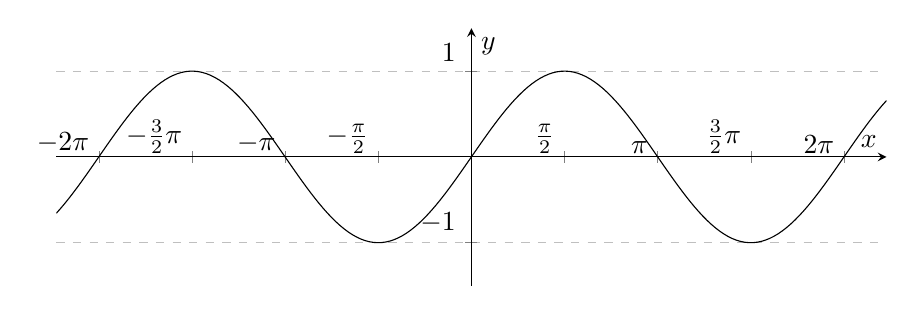
\begin{tikzpicture}
\begin{axis}[xmax = 7, xmin = -7, ymax = 1.5, ymin = -1.5,
             axis lines=middle, xlabel=$x$, ylabel=$y$,
             xtick={-2*pi, -3*pi/2, -pi, -pi/2, 0, pi/2, pi, 3*pi/2, 2*pi},
             xticklabels={$-2\pi$, $-\frac{3}{2}\pi$, $-\pi$, $-\frac{\pi}{2}$, $0$, $\frac{\pi}{2}$, $\pi$, $\frac{3}{2}\pi$, $2\pi$},
             xticklabel style={anchor=south east},
             ytick={-1, 1},
             yticklabel style={anchor=south east},
             ymajorgrids=true,
             grid style=dashed,
             width=\linewidth,
             height=0.4\linewidth
            ]
\addplot[domain=-7:7, samples=200]{sin(deg(x))};
\end{axis}
\end{tikzpicture}
\caption{Grafico di $y= \sin{x}$}
\end{figure}

\begin{figure}
\centering
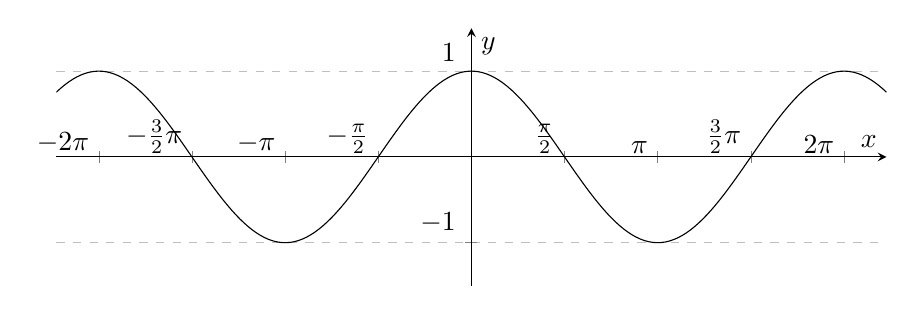
\begin{tikzpicture}
\begin{axis}[xmax = 7, xmin = -7, ymax = 1.5, ymin = -1.5,
             axis lines=middle, xlabel=$x$, ylabel=$y$,
             xtick={-2*pi, -3*pi/2, -pi, -pi/2, 0, pi/2, pi, 3*pi/2, 2*pi},
             xticklabels={$-2\pi$, $-\frac{3}{2}\pi$, $-\pi$, $-\frac{\pi}{2}$, $0$, $\frac{\pi}{2}$, $\pi$, $\frac{3}{2}\pi$, $2\pi$},
             xticklabel style={anchor=south east},
             ytick={-1, 1},
             yticklabel style={anchor=south east},
             ymajorgrids=true,
             grid style=dashed,
             width=\linewidth,
             height=0.4\linewidth
            ]
\addplot[domain=-7:7, samples=200]{cos(deg(x))};
\end{axis}
\end{tikzpicture}
\caption{Grafico di $y= \cos{x}$}
\end{figure}

\begin{figure}[H]
\centering
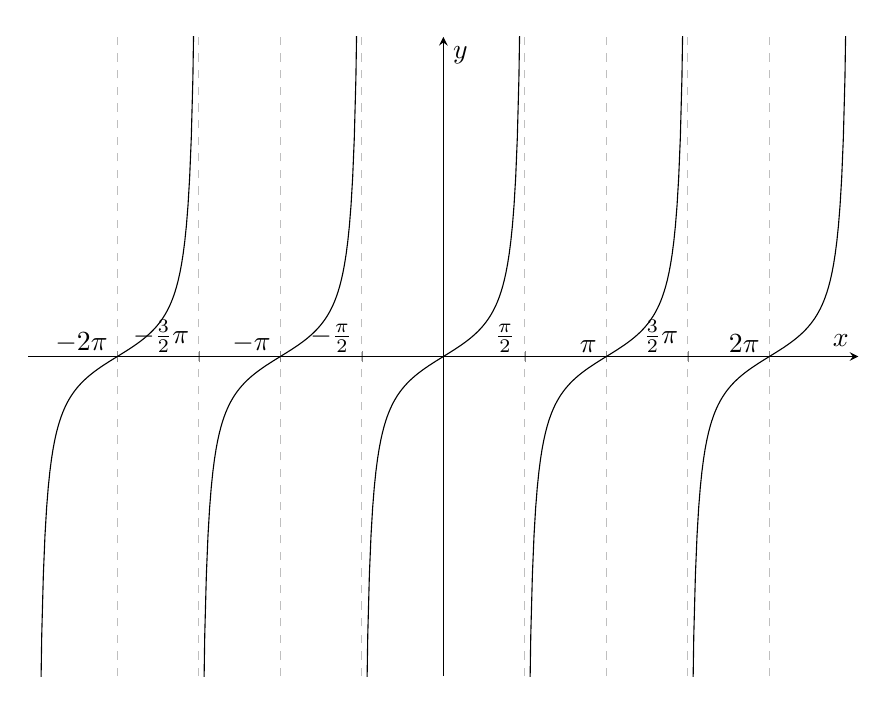
\begin{tikzpicture}
\begin{axis}[xmax = 8, xmin = -8, ymax = 10, ymin = -10,
             axis lines=middle, xlabel=$x$, ylabel=$y$,
             xtick={-2*pi, -3*pi/2, -pi, -pi/2, 0, pi/2, pi, 3*pi/2, 2*pi},
             xticklabels={$-2\pi$, $-\frac{3}{2}\pi$, $-\pi$, $-\frac{\pi}{2}$, $0$, $\frac{\pi}{2}$, $\pi$, $\frac{3}{2}\pi$, $2\pi$},
             y tick style={draw=none},
             yticklabels={},
             xticklabel style={anchor=south east},
             xmajorgrids=true,
             grid style=dashed,
             width=\linewidth,
             height=0.8\linewidth
            ]
\addplot[domain=-pi/2+0.02:pi/2-0.02, samples=100]{tan(deg(x))};
\addplot[domain=-pi/2+0.02+pi:pi/2-0.02+pi, samples=100]{tan(deg(x))};
\addplot[domain=-pi/2+0.02-pi:pi/2-0.02-pi, samples=100]{tan(deg(x))};
\addplot[domain=-pi/2+0.02+2*pi:pi/2-0.02+2*pi, samples=100]{tan(deg(x))};
\addplot[domain=-pi/2+0.02-2*pi:pi/2-0.02-2*pi, samples=100]{tan(deg(x))};
\end{axis}
\end{tikzpicture}
\caption{Grafico di $y= \tan{x}$}
\end{figure}

\subsubsection{Formule utili}
Dalla prima identità è possibile ricavare una formula per passare dal seno al coseno, il problema è che per farlo bisogna prima sapere in che quadrante ci si trova e, di conseguenza, decidere il segno della radice:
\begin{equation*}
    \sin{x} = \pm \sqrt{1-\cos^2{x}}
\end{equation*}

Di seguito le formule di \textbf{addizione} e \textbf{sottrazione}: \label{sec_formuleAddSott}
\begin{gather*}
    \cos(\alpha + \beta) = \cos{\alpha}\cos{\beta} - \sin{\alpha}\sin{\beta}\\
    \cos(\alpha - \beta) = \cos{\alpha}\cos{\beta} + \sin{\alpha}\sin{\beta}\\
    \sin(\alpha + \beta) = \sin{\alpha}\cos{\beta} + \cos{\alpha}\sin{\beta}\\
    \sin(\alpha - \beta) = \sin{\alpha}\cos{\beta} - \cos{\alpha}\sin{\beta}
\end{gather*}

Formule di \textbf{duplicazione}:\label{sec_formuleDuplicazione}
\begin{align*}
    \sin(2\alpha) &= 2\sin{\alpha}\cos{\alpha}\\
    \cos(2\alpha) &= \cos^2{\alpha} - \sin^2{\alpha} =\\
    &= 1 - 2\sin^2{\alpha} = \\
    &= 2\cos^2{\alpha} - 1
\end{align*}
Le ultime due formule per la duplicazione del coseno sono ricavate sostituendo a $\cos^2{\alpha} - \sin^2{\alpha}$ la prima identità fondamentale ($\sin^2{x} + \cos^2{x} = 1$). Si noti come la formula di duplicazione del coseno permette di passare \textbf{da un quadrato a una funzione lineare} e viceversa.

Ulteriore formule:
\begin{gather*}
    \sin\left(\frac{\pi}{2}-\alpha\right) = \cos{\alpha}\\
    \cos\left(\frac{\pi}{2}-\alpha\right) = \sin{\alpha}\\
\end{gather*}

\subsubsection{Funzioni goniometriche inverse}

Essendo seno e coseno periodiche ovviamente non sono invertibili, in quanto per essere invertibili dovrebbero essere iniettive e suriettive. In realtà seno e coseno sono suriettive, ma non iniettive. È quindi necessario restringere il loro dominio per renderle iniettive.

Per convenzione il dominio del \textbf{seno} si restringe all'intervallo $[-\frac{\pi}{2}, \frac{\pi}{2}]$. Si noti che si potrebbe scegliere un qualsiasi altro intervallo purché il seno "ristretto" sia ancora iniettivo (es. si può prendere come intervallo $[\frac{\pi}{2}, \frac{3}{2}\pi]$ ma non $[0, \pi]$).
\begin{equation*}
    \sin |_{[-\frac{\pi}{2}, \frac{\pi}{2}]}: [-\frac{\pi}{2}, \frac{\pi}{2}] \to [-1, 1]
\end{equation*}
Essendo diventata biunivoca è possibile invertirla:
\dfn{
    La funzione inversa al seno è l'\textbf{arcoseno}:
    \begin{equation*}
        \left( \sin |_{[-\frac{\pi}{2}, \frac{\pi}{2}]} \right)^{-1} (y) = \arcsin{y}
    \end{equation*}
    \begin{equation*}
        \arcsin: [-1, 1] \to [-\frac{\pi}{2}, \frac{\pi}{2}]
    \end{equation*}
}
Essendo che il codominio dell'arcoseno è $[-\frac{\pi}{2}, \frac{\pi}{2}]$:
\begin{equation*}
    \begin{cases}
        \forall x \in [-1, 1]\\
        \sin(\arcsin{x}) = x
    \end{cases}
    \qquad \qquad
    \begin{cases}
        \forall x \in [-\frac{\pi}{2}, \frac{\pi}{2}] \;\;(\mathrm{non}\; \mathbb{R})\\
        \arcsin(\sin{x}) = x
    \end{cases}
\end{equation*}
Per esempio: $\arcsin(\sin{\pi}) = \arcsin{0} = 0 \neq \pi$.\\

Lo stesso discorso vale per il \textbf{coseno} e la \textbf{tangente}. Mente però per la tangente possiamo tenere lo stesso intervallo del seno come dominio ristretto, per il coseno è necessario usare un altro intervallo in quanto $[-\frac{\pi}{2}, \frac{\pi}{2}]$ non lo renderebbe iniettivo:
\dfn{
    La funzione inversa al coseno è l'\textbf{arcocoseno}:
    \begin{equation*}
        \left( \cos |_{[0, \pi]} \right)^{-1} (y) = \arccos{y}
    \end{equation*}
    \begin{equation*}
        \arccos: [-1, 1] \to [0, \pi]
    \end{equation*}
}

\begin{equation*}
    \begin{cases}
        \forall x \in [-1, 1]\\
        \cos(\arccos{x}) = x
    \end{cases}
    \qquad \qquad
    \begin{cases}
        \forall x \in [0, \pi] \;\;(\mathrm{non}\; \mathbb{R})\\
        \arccos(\cos{x}) = x
    \end{cases}
\end{equation*}

\dfn{
    La funzione inversa alla tangente è l'\textbf{arcotangente}:
    \begin{equation*}
        \left( \tan |_{[-\frac{\pi}{2}, \frac{\pi}{2}]} \right)^{-1} (y) = \arctan{y}
    \end{equation*}
    \begin{equation*}
        \arctan: \mathbb{R} \to [-\frac{\pi}{2}, \frac{\pi}{2}]
    \end{equation*}
}

\begin{equation*}
    \begin{cases}
        \forall x \in \mathbb{R}\\
        \tan(\arctan{x}) = x
    \end{cases}
    \qquad \qquad
    \begin{cases}
        \forall x \in [-\frac{\pi}{2}, \frac{\pi}{2}] \;\;(\mathrm{non}\; \mathbb{R})\\
        \arctan(\tan{x}) = x
    \end{cases}
\end{equation*}

I grafici delle funzioni inverse sono i seguenti:
\begin{figure}[h]
\centering
\begin{tikzpicture}
\begin{axis}[xmax = 1.5, xmin = -1.5, ymax = 2, ymin = -2,
             axis lines=middle, xlabel=$x$, ylabel=$y$,
             xtick={-1, 1},
             xticklabels={$-1$, $1$},
             xticklabel style={anchor=south east},
             ytick={-pi/2, pi/2},
             yticklabels={$-\frac{\pi}{2}$, $\frac{\pi}{2}$},
             yticklabel style={anchor=south east},
             width=0.5\linewidth,
             height=0.5\linewidth
            ]
\addplot[domain=-1:1, samples=200]{asin(x)/180*pi};
\end{axis}
\end{tikzpicture}
\caption{Grafico di $y= \arcsin{x}$}
\end{figure}

\begin{figure}[h]
\centering
\begin{tikzpicture}
\begin{axis}[xmax = 1.5, xmin = -1.5, ymax = 4, ymin = -0.5,
             axis lines=middle, xlabel=$x$, ylabel=$y$,
             xtick={-1, 1},
             xticklabels={$-1$, $1$},
             xticklabel style={anchor=north},
             ytick={pi/2, pi},
             yticklabels={$\frac{\pi}{2}$, $\pi$},
             yticklabel style={anchor=south west},
             width=0.5\linewidth,
             height=0.5\linewidth
            ]
\addplot[domain=-1:1, samples=200]{acos(x)/180*pi};
\end{axis}
\end{tikzpicture}
\caption{Grafico di $y= \arccos{x}$}
\end{figure}

\begin{figure}[h]
\centering
\begin{tikzpicture}
\begin{axis}[xmax = 15, xmin = -15, ymax = 3, ymin = -3,
             axis lines=middle, xlabel=$x$, ylabel=$y$,
             xtick style={draw=none},
             xticklabels={},
             xticklabel style={anchor=north},
             ytick={-pi/2, pi/2},
             yticklabels={$-\frac{\pi}{2}$, $\frac{\pi}{2}$},
             yticklabel style={anchor=south west},
             ymajorgrids=true,
             grid style=dashed,
             width=\linewidth,
             height=0.5\linewidth
            ]
\addplot[domain=-15:15, samples=200]{atan(x)/180*pi};
\end{axis}
\end{tikzpicture}
\caption{Grafico di $y= \arctan{x}$}
\end{figure}

\subsection{Esponenziale}
Come abbiamo ricavato dalla radice aritmetica (sezione \ref{sec_radiceAritmetica}), siamo in grado di definire l'esponenziale per un qualsiasi esponente razionale positivo. Infatti qualsiasi numero razionale positivo è esprimibile nella forma $q = \frac{m}{n}$ e quindi, sempre per la radice aritmetica:
\begin{equation*}
    a^q = a^{\frac{m}{n}} = \sqrt[n]{a^m} \qquad \forall q \in \mathbb{Q}_{+}, \forall a \in \mathbb{R}_{+},\; \mathrm{con}\; n,m \in \mathbb{N}\;\, \mathrm{e}\;\, n \neq 0
\end{equation*}
\textbf{La base dell'esponenziale è necessario che sia positiva} in quanto se non lo fosse la definizione arriverebbe ad una contraddizione. Per esempio se volessi calcolare $(-2)^3 = -8$ come un esponenziale seguendo la definizione che abbiamo:
\begin{equation*}
    (-2)^3 = (-2)^{\frac{6}{2}} = \sqrt{(-2)^6} = \sqrt{64} = 8 \neq -8
\end{equation*}
Il primo passo per estendere questa definizione è chiederci come possiamo definire l'esponenziale per tutto l'insieme dei razionali, cioè anche per esponenti razionali negativi. La risposta è abbastanza semplice perché ci basta dire che se l'esponente è negativo calcoliamo il reciproco con l'esponente positivo:
\begin{equation*}
    a^{-q} = a^{-\frac{m}{n}} = \dfrac{1}{a^{\frac{m}{n}}} = \dfrac{1}{\sqrt[n]{a^m}} \qquad \forall q \in \mathbb{Q}_{+}, \forall a \in \mathbb{R}_{+},\; \mathrm{con}\; n,m \in \mathbb{N}\;\, \mathrm{e}\;\, n \neq 0
\end{equation*}
Siamo quindi riusciti a definire l'esponenziale per tutti gli esponenti razionali, sia positivi che negativi. Ora ci manca estendere questa definizione ai numeri reali. Purtroppo per farlo sono necessarie due nozioni non ancora introdotte: quella di successione e quella di limite. Per comprendere quindi a pieno i passaggi successivi è necessario andare prima guardarsi le sezioni relative (cioè la sezione \ref{sec_successioni} per le successioni e la sezione \ref{sec_limiti} per i limiti).\\

La domanda è come facciamo a definire $3^{\sqrt{2}}$ o $5^{\sqrt{27}}$? Cioè come facciamo a definire l'esponenziale per gli esponenti appartenenti all'insieme $\mathbb{R}\setminus\mathbb{Q}$? L'idea è di \textbf{approssimare l'esponente con una successione} di numeri razionali. Se per esempio voglio calcolare $3^{\sqrt{2}}$, ho come esponente $\sqrt{2}$, quindi la successione diventa:
\begin{align*}
    q_1 &= 1\\
    q_2 &= 1,4\\
    q_3 &= 1,41\\
    q_4 &= 1,414\\
    q_5 &= 1,4142\\
    q_6 &= 1,41421\\
    \vdots
\end{align*}
È facile vedere che questa successione è \textbf{crescente} ($3^{q_n} \leq 3^{q_{n+1}}$) visto che il termine successivo ha sempre una cifra in più e inoltre questa successione è \textbf{superiormente limitata} visto che $3^{q_n} \leq 3^2 = 9$. Essendo crescente e superiormente limitata questa successione ha limite e quindi $3^{\sqrt{2}}$ si definisce proprio come il limite di questa successione:
\begin{equation*}
    3^{\sqrt{2}} \vcentcolon = \lim_{n\to +\infty} 3^{q_n}
\end{equation*}
Arriviamo quindi a definire il caso generale dell'esponenziale: \label{sec_esponenziale}
\dfn{
    Si definisce \textbf{esponenziale} in base $a$ di $x$ ($\exp_a{x}$) e si indica con $a^x$, $\forall a > 0 \in \mathbb{R}$:
    \begin{enumerate}
        \item Se $x \in \mathbb{Q}_{+}$:
            \begin{equation*}
                a^x = a^{\frac{m}{n}} = \sqrt[n]{a^m} \qquad \mathrm{con}\; n,m \in \mathbb{N}: x = \frac{m}{n}\;\, \mathrm{e}\;\, n \neq 0
            \end{equation*}
        \item Se $x \in \mathbb{Q}_{-}$:
            \begin{equation*}
                a^{x} = a^{-\frac{m}{n}} = \dfrac{1}{a^{\frac{m}{n}}} = \dfrac{1}{\sqrt[n]{a^m}} \qquad \mathrm{con}\; n,m \in \mathbb{N}: x = -\frac{m}{n}\;\, \mathrm{e}\;\, n \neq 0
            \end{equation*}
        \item Se $x \in \mathbb{R}\setminus\mathbb{Q}$:\\
            Data $(q_n)_n \subseteq \mathbb{Q} : q_n \nearrow, q_n \to x$:
            \begin{equation*}
                a^x \vcentcolon = \lim_{n \to +\infty} a^{q_n}
            \end{equation*}
    \end{enumerate}
}

\imp{\begin{center}
    L'esponenziale in \textbf{base naturale} è quello in base $e$
\end{center}}
Il numero $e$ è descritto nella sezione relativa al numero di Eulero (Sezione \ref{sec_numeroDiEulero}) e si dice che l'esponenziale in questa base è "naturale" perché ha moltissime proprietà che vedremo in seguito.

\begin{figure}
\centering
\begin{subfigure}{0.49\textwidth}
\centering
	\begin{tikzpicture}
	\begin{axis}[xmax = 5, xmin = -5, ymax = 4, ymin = -0.5,
		     axis lines=middle, xlabel=$x$, ylabel=$y$,
		     xtick style={draw=none},
		     xticklabels={},
		     ytick={1},
		     yticklabels={$1$},
		     yticklabel style={anchor=north west},
		    ]
	\addplot[domain=-5:5, samples=200]{2^x};
	\end{axis}
	\end{tikzpicture}
\end{subfigure}
\begin{subfigure}{0.49\textwidth}
\centering
	\begin{tikzpicture}
	\begin{axis}[xmax = 5, xmin = -5, ymax = 4, ymin = -0.5,
		     axis lines=middle, xlabel=$x$, ylabel=$y$, xlabel style={anchor=north west},
		     xtick style={draw=none},
		     xticklabels={},
		     ytick={1},
		     yticklabels={$1$},
		     yticklabel style={anchor=south west},
		    ]
	\addplot[domain=-5:5, samples=200]{0.5^x};
	\end{axis}
	\end{tikzpicture}
\end{subfigure}
	\caption{Grafico (da sinistra a destra) di $y= a^x$ con $a > 1$ e di $y= b^x$ con $0 < b < 1$} 
\end{figure}

\subsection{Logaritmo}
Come molte funzioni anche l'esponenziale ha una sua funzione inversa, e cioè che permette di trovare l'esponente data la base e il risultato. La funzione inversa all'esponenziale è il \textbf{logaritmo}:
\thm{
    Dato $a \in \mathbb{R}: a > 0, a \neq 1$, $\forall y \in \mathbb{R}: y > 0$, $\exists \oc x \in \mathbb{R}$: $a^x = y$. Definiamo \textbf{logaritmo} in base $a$ di $y$:
    \begin{equation*}
        \log_{a}(y) \vcentcolon = x
    \end{equation*}
    
    La funzione logaritmo ha come dominio $\mathbb{R}_{+}^* = \{r \in \mathbb{R}: r > 0\}$ e come codominio $\mathbb{R}$:
    \begin{equation*}
        \log: \mathbb{R}_{+}^* \to \mathbb{R}
    \end{equation*}
}

Essendo quindi il logaritmo l'inverso dell'esponenziale:
\begin{gather*}
    a^{\log_a(y)} = y \qquad \forall y \in \mathbb{R}_{+}^{*}\\
    \log_a(a^x) = x \qquad \forall x \in \mathbb{R}
\end{gather*}
Il logaritmo naturale, cioè in base $e$ si indica come $\ln{x}$.


\begin{figure}
\centering
\begin{subfigure}{0.49\textwidth}
\centering
	\begin{tikzpicture}
	\begin{axis}[xmax = 4, xmin = -0.5, ymax = 4, ymin = -4,
		     axis lines=middle, xlabel=$x$, ylabel=$y$, ylabel style={anchor=east},
		     ytick style={draw=none},
		     yticklabels={},
		     xtick={1},
		     xticklabels={$1$},
		     xticklabel style={anchor=north west},
		    ]
	\addplot[samples=800]{ln(x)};
	\end{axis}
	\end{tikzpicture}
\end{subfigure}
\begin{subfigure}{0.49\textwidth}
\centering
	\begin{tikzpicture}
	\begin{axis}[xmax = 4, xmin = -0.5, ymax = 4, ymin = -4,
		     axis lines=middle, xlabel=$x$, ylabel=$y$, ylabel style={anchor=east},
		     ytick style={draw=none},
		     yticklabels={},
		     xtick={1},
		     xticklabels={$1$},
		     xticklabel style={anchor=north west},
		    ]
	\addplot[samples=800]{ln(x)/ln(0.5)};
	\end{axis}
	\end{tikzpicture}
\end{subfigure}
	\caption{Grafico (da sinistra a destra) di $y= \log_a(x)$ con $ a > 1$ e di $y= \log_b(x)$ con $0 < b < 1$} 
\end{figure}

Ci sarebbe da discutere sulle proprietà del logaritmo, ma mi limiterò ad elencarle di seguito:
\imp{
	\begin{align*}
		&\log_a(x \cdot y) = \log_a(x) + \log_a (y)\\[5pt]
		&\log_a \left(\dfrac{x}{y} \right) = \log_a(x) - \log_a (y)\\[5pt]
		&\log_a \left(x^y \right) = y \cdot \log_a(x)\\[5pt]
		&\log_a \left(x \right) = \dfrac{\log_b(x)}{\log_b(a)}
	\end{align*}
}


\section{Successioni e serie} \label{successioni}
\dfn{
    Una successione di numeri reali è una funzione:
    \begin{gather*}
        f: \mathbb{N} \to \mathbb{R}\\
        n \to f(n) = \vcentcolon a_n
    \end{gather*}
    E si indicato in tre possibili modi:
    \begin{equation*}
        (a_n)_{n \in \mathbb{N}},\;\, (a_n)_n\;\, \text{oppure}\;\, (a_n)
    \end{equation*}
}
L'idea alla base delle successione matematiche è poter scrivere una lista di numeri che però abbiano un ordine. Avendole infatti definite come funzioni si può tenere l'ordine dei termini della successione semplicemente:
\begin{gather*}
    f(0) = a_0\\
    f(1) = a_1\\
    f(2) = a_2\\
    f(3) = a_3\\
    \vdots
\end{gather*}
Il poter scrivere numeri in successione e dare loro un ordine sembra apparentemente sembra inutile, ma in realtà si rivela estremamente utile in moltissime definizioni di funzioni che però vanno estese. Per esempio, come è spiegato nella sezione \ref{esponenziale} riguardo all'esponenziale, per definire tale funzione per tutti i numeri reali è necessario utilizzare una successione.\\

\dfn{
    Data una successione $(a_n)_n$ e un insieme $A = \{ a_n | n \in \mathbb{N}\}$. $(a_n)$ si dice:
    \begin{itemize}
        \item \textbf{Superiormente limitata} se $A$ è superiormente limitato.
        \item \textbf{Inferiormente limitata} se $A$ è inferiormente limitato.
        \item \textbf{Limitata} se $A$ è limitato.
    \end{itemize}
}

\subsection{Successioni monotone}
Per capire quanto segue è necessario prima guardare la sezioni sui limiti delle successioni (\ref{lim_successioni}).
\dfn{
$(a_n)_n$ si dice \textbf{crescente} e si indica con $(a_n \nearrow)$ se:
\begin{equation*}
    \forall n \in \mathbb{N} : a_n \leq a_{n+1}
\end{equation*}
}
\dfn{
$(a_n)_n$ si dice \textbf{strettamente crescente} e si indica sempre con $(a_n \nearrow)$ se:
\begin{equation*}
    \forall n \in \mathbb{N} : a_n < a_{n+1}
\end{equation*}
}
\dfn{
$(a_n)_n$ si dice \textbf{decrescente} e si indica con $(a_n \searrow)$ se:
\begin{equation*}
    \forall n \in \mathbb{N} : a_n \geq a_{n+1}
\end{equation*}
}
\dfn{
$(a_n)_n$ si dice \textbf{strettamente decrescente} e si indica sempre con $(a_n \searrow)$ se:
\begin{equation*}
    \forall n \in \mathbb{N} : a_n > a_{n+1}
\end{equation*}
}

Una successione crescente o decrescente si dice \textbf{monotona}. Le successioni monotone \textbf{hanno sempre limite}.

\thm{
Se $(a_n)_n$ è \textbf{crescente}, allora:
\begin{equation*}
    \lim_{x\to +\infty} a_n = \sup \{a_n | n \in \mathbb{N}\}
\end{equation*}
Se $(a_n)_n$ è \textbf{decrescente}, allora:
\begin{equation*}
    \lim_{x\to +\infty} a_n = \inf \{a_n | n \in \mathbb{N}\}
\end{equation*}
}
Dimostriamo il teorema appena enunciato:
\pf{
Dimostreremo il teorema soltanto per $(a_n)_n \nearrow$. Si tratta quindi di provare:
\begin{equation*}
    \lim_{x\to +\infty} a_n = \sup \{a_n | n \in \mathbb{N}\}
\end{equation*}
Poniamo $L \coloneq \sup \{a_n | n \in \mathbb{N}\}$
Bisogna dimostrare due casi: $L = +\infty$ e $L \in \mathbb{R}$
\begin{enumerate}
    \item $\mathbf{L = + \infty}$
        Ci riduciamo a provare che 
        \begin{equation*}
            \lim_{x\to +\infty} a_n = +\infty
        \end{equation*}
        cioè
        \begin{equation*}
            \forall K > 0, \exists \bar{n} = \bar{n} (\epsilon) \in \mathbb{N} : \forall \bar{n} \geq n : a_n > K
        \end{equation*}
        Dato $A = \{a_n | n \in \mathbb{N}\}$
        \begin{itemize}
            \item A non è superiormente limitato in quanto $L = +\infty$
            \item A di conseguenza non ammette maggioranti
            \item Ne consegue che K non è un maggiorante $\implies \exists \bar{n} \in A : a_{\bar{n}} > K$
            \item Siccome per ipotesi $(a_n)_n \nearrow \implies \forall n \geq \bar{n} : a_n \geq a_{\bar{n}} > K$ 
        \end{itemize}
    \item $\mathbf{L \in \mathbb{R}}$
    Ci riduciamo a provare che 
        \begin{equation*}
            \lim_{x\to +\infty} a_n = L
        \end{equation*}
        cioè
        \begin{align*}
            \forall \epsilon > 0, \exists \bar{n} = \bar{n} (\epsilon) \in \mathbb{N} : \forall \bar{n} \geq n : |a_n& - L| < \epsilon\\
            &\Big\Updownarrow\\
            L - \epsilon < &a_n < L + \epsilon
        \end{align*}
        $a_n < L + \epsilon$ è ovvio per ipotesi in quanto $L$ è un maggiorante, quindi $\forall n: a_n \leq L < L + \epsilon$. Ci rimane quindi solo da trovare $\bar{n}$ tale che:
        \begin{equation*}
            \forall n \geq \bar{n} : a_n > L - \epsilon
        \end{equation*}
        Essendo $L = \sup A = \sup \{a_n | \in \mathbb{N}\}$
        \begin{itemize}
            \item $L$ è il più piccolo dei maggioranti di $A$
            \item $L - \epsilon$ non è quindi un maggiorante di $A$ $\implies \exists a_{\bar{n}} \in A : L -\epsilon < a_{\bar{n}}$
            \item Essendo $(a_n)_n \nearrow$ si ha che $\forall n > \bar{n} \;\; L-\epsilon < a_{\bar{n}} \leq a_{n}$
        \end{itemize}
        quindi
        \begin{equation*}
            a_n > L - \epsilon
        \end{equation*}
        
        \hfill Q.e.d.
\end{enumerate}
}
\textbf{Corollari} \label{corollario_successioni}
\begin{enumerate}
    \item Se $(a_n)_n \nearrow$ e $(a_n)_n$ è \textbf{superiormente limitata}, allora $(a_n)_n$ è \textbf{convergente}, cioè
        \begin{equation*}
            \exists r \in \mathbb{R} : a_n \xrightarrow{\quad} r
        \end{equation*}
    \item Se $(a_n)_n \searrow$ e $(a_n)_n$ è \textbf{inferiormente limitata}, allora $(a_n)_n$ è \textbf{convergente}, cioè
        \begin{equation*}
            \exists r \in \mathbb{R} : a_n \xrightarrow{\quad} r
        \end{equation*}
\end{enumerate}

\section{Limiti} \label{limiti}
Prendiamo una successione abbastanza semplice da definire, tipo:
\begin{equation*}
    a_n = \frac{n-1}{n}
\end{equation*}
Cominciamo ora ad elencare i suoi termi e calcolariamo i suoi valori:
\begin{align*}
    a_1 &= \dfrac{0}{1} = 0\\
    a_2 &= \dfrac{1}{2} = 0.5\\
    a_3 &= \dfrac{2}{3} = 0.\overline{6}\\
    a_4 &= \dfrac{3}{4} = 0.75\\
    \vdots\\
    a_{1000} &= \dfrac{999}{1000} = 0.999\\
    \vdots\\
    a_{100000} &= \dfrac{99999}{100000} = 0.99999\\
\end{align*}
È facile notare che più $n$ diventa grande più il valore della successione \textit{tende} a $1$. Come si formalizza questa cosa? Con il concetto di limite.

\subsection{Limite di una successione} \label{lim_successioni}
\dfn{
    Data una successione $(a)_n$, e un numero $L \in \mathbb{R}$, si dice che $(a)_n$ è \textbf{convergente} e si indica:
    \begin{equation*}
        \lim_{x \to +\infty} a_n = L \qquad \text{oppure} \qquad (a)_n \xrightarrow[n \to +\infty]{} L
    \end{equation*}
    \qquad se
    \begin{equation*}
        \forall \epsilon > 0, \exists \bar{n} = \bar{n}(\epsilon) \in \mathbb{N}: \forall n \geq \bar{n}: |a_n - L| < \epsilon
    \end{equation*}
}

\dfn{
    Data una successione $(a)_n$, si dice che $(a)_n$ è \textbf{divergente} e si indica:
    \begin{itemize}
        \item \begin{equation*}
                \lim_{x \to +\infty} a_n = +\infty \qquad \text{oppure} \qquad (a)_n \xrightarrow[n \to +\infty]{} +\infty
            \end{equation*}
            \qquad se
            \begin{equation*}
                \forall \epsilon > 0, \exists \bar{n} = \bar{n}(\epsilon) \in \mathbb{N}: \forall n \geq \bar{n}: a_n \geq \epsilon
            \end{equation*}
        \item \begin{equation*}
                \lim_{x \to +\infty} a_n = -\infty \qquad \text{oppure} \qquad (a)_n \xrightarrow[n \to +\infty]{} -\infty
            \end{equation*}
            \qquad se
            \begin{equation*}
                \forall \epsilon > 0, \exists \bar{n} = \bar{n}(\epsilon) \in \mathbb{N}: \forall n \geq \bar{n}: a_n \leq -\epsilon
            \end{equation*}
    \end{itemize}
}

\imp{
\begin{center}
    Se esiste il limite di una successione esso è \textbf{unico}
\end{center}
}

Esistono successioni che non hanno limite (non sono ne convergenti ne divergenti).
\begin{gather*}
    a_n = (-1)^2\\
    a_0 = 1,\; a_1 = -1,\; a_2 = 1 \;\cdots
\end{gather*}
La successione è limitata in quanto i suoi valori sono $-1 e 1$, eppure non ha limite in quanto oscilla.
\begin{gather*}
    a_n = (-1)^n \cdot n\\
    a_0 = 0,\; a_1 = -1,\; a_2 = 2,\; a_3 = -3,\; a_4 = 4 \;\cdots
\end{gather*}
La successione in quanto caso non è limitata e non ha un limite in quanto "salta" tra valori positivi e valori negativi.

\subsection{Numero di Eulero (o Nepero)} \label{NumeroDiEulero}
%DA FARE MOLTO MEGLIO
Prendiamo in considerazione la serie
\begin{equation*}
    a_n = (1+\dfrac{1}{n})^n
\end{equation*}
Dimostriamo che è una serie \textbf{convergente}, e chiamiamo il suo limite \textbf{\textit{e}}. Quindi:
\begin{equation*}
    \lim_{x\to +\infty} (1+\dfrac{1}{n})^n = e \in \mathbb{R}
\end{equation*}

\pf{
Per dimostrare che una successione è convergente ci basta dimostrare che è (strettamente) crescente e limitata. Questo dal corollario della dimostrazione nella sezione \ref{corollario_successioni}.
\begin{enumerate}
    \item Dimostriamo che $(a_n)$ è (strettamente) crescente:
    
    \mlem{
        È necessario, per questa dimostrazione, introdurre la \textit{disuguaglianza di Bernulli}. Tuttavia non la dimostreremo.
        \begin{equation*}
            \forall x \in R : x \geq -1, \forall x \in \mathbb{N}: (1+x)^n \geq 1 + nx
        \end{equation*}
    }
    Per dimostrare che $(a_n)_n \nearrow$ ci basta dimostrare che:
    \begin{equation*}
        \dfrac{a_{n+1}}{a_n} > 1
    \end{equation*}
    \begin{align*}
        \dfrac{a_{n+1}}{a_n} &= \dfrac{\left(1+\dfrac{1}{n+1}\right)^{n+1}}{\left(1+\dfrac{1}{n}\right)^n} = \dfrac{\left(\dfrac{n+2}{n+1}\right)^{n+1}}{\left(\dfrac{n+1}{n}\right)^n}
        = \dfrac{\dfrac{n+2}{n+1} \cdot \left( \dfrac{n+2}{n+1} \right)^n}{\left(\dfrac{n+1}{n}\right)^n} =\\[5pt]
        &= \dfrac{n+2}{n+1} \cdot \left( \dfrac{n+2}{n+1} \cdot \dfrac{n}{n+1} \right)^n = \dfrac{n+2}{n+1} \cdot \left( \dfrac{n^2+2n+1-1}{n^2+2n+1} \right)^n =\\[5pt]
        &= \dfrac{n+2}{n+1} \cdot \left( 1 -\dfrac{1}{n^2+2n+1} \right)^n = \dfrac{n+2}{n+1} \cdot \left( 1 + \left( -\dfrac{1}{n^2+2n+1}\right) \right)^n
    \end{align*}
    Usiamo la disuguaglianza di Bernulli. Però assicuriamoci prima di poterla usare:
    \begin{gather*}
        x = - \dfrac{1}{n^2+2n+1} \geq -1\\
        \dfrac{1}{n^2+2n+1} \leq 1\\
        \leq n^2+2n+1\\
        n^2+2n >= 0
    \end{gather*}
    Verificato! Ora usiamola:
    \begin{align*}
        &\dfrac{n+2}{n+1} \cdot \left( 1 + \left( -\dfrac{1}{n^2+2n+1}\right) \right)^n \geq \dfrac{n+2}{n+1} \cdot \left( 1 + n\left( -\dfrac{1}{n^2+2n+1}\right) \right)=\\[5pt]
        &= \dfrac{n+2}{n+1} \cdot \dfrac{n^2+2n+1-n}{n^2+2n+1} = \dfrac{n+2}{n+1} \cdot \dfrac{n^2+n+1}{n^2+2n+1} =\\[5pt]
        & = \dfrac{n^3+3n^2+3n+1+1}{n^3+3n^2+3n+1} = 1 + \dfrac{1}{n^3+3n^2+3n+1} > 1
    \end{align*}
    
    \item Dobbiamo provare ora che $(a_n)_n$ è limitata. Usiamo il binomio di newton:
    \begin{align*}
        (1+\dfrac{1}{n})^n &= \sum_{k = 0}^{n} \binom{n}{k} \cdot 1^{n-k} \cdot \left(\dfrac{1}{n}\right)^k = \sum_{k = 0}^{n} \binom{n}{k}\dfrac{1}{n^k} = \sum_{k = 0}^{n} \dfrac{n!}{(n-k)!k!}\cdot\dfrac{1}{k!}=\\
        &= \sum_{k = 0}^{n} \dfrac{n \cdot (n-1) \cdots (n-k+1)}{n^k} \cdot \dfrac{1}{k!} =\\
        &= \sum_{k = 0}^{n} \dfrac{n}{n} \cdot \dfrac{(n-1)}{n} \cdots \dfrac{(n-k+1)}{n} \cdot \dfrac{1}{k!} =
    \end{align*}
        È facile notare che:
    \begin{equation*}
        \dfrac{n}{n} \cdot \dfrac{(n-1)}{n} \cdots \dfrac{(n-k+1)}{n} \leq 1
    \end{equation*}
    In quanto il denominatore sarà sempre più grande del numeratore (tranne per il primo termine) e quindi ogni singolo termine sarà $\leq 1$ ed essendo tutti moltiplicati tra di loro il risultato sarà anch'esso $\leq 1$. Possiamo quindi concludere che:
    \begin{equation*}
        = \sum_{k = 0}^{n} \dfrac{n}{n} \cdot \dfrac{(n-1)}{n} \cdots \dfrac{(n-k+1)}{n} \cdot \dfrac{1}{k!} \leq \sum_{k = 0}^{n} \dfrac{1}{k!} = 2 + \sum_{k = 2}^{n} \dfrac{1}{k!}
    \end{equation*}
    Possiamo notare che:
    \begin{equation*}
        k! = k\cdot (k-1)\cdot (k-2) \cdots 1 \geq k (k-1) > 0 \qquad \text{per} k\geq 2
    \end{equation*}
    \begin{equation*}
        \implies k! > k(k-1) \implies \dfrac{1}{k!} < \dfrac{1}{k(k-1)} = \dfrac{1}{k-1} - \dfrac{1}{k}
    \end{equation*}
    Quindi sostituendo
    \begin{align*}
        &< 2 + \sum_{k = 0}^{n} \left(\dfrac{1}{k-1} - \dfrac{1}{k}\right) = 2 + \left[ \left(1-\dfrac{1}{2}\right) + \left(\dfrac{1}{2}-\dfrac{1}{3}\right) + \left(\dfrac{1}{3}-\dfrac{1}{4}\right) \cdots \left(\dfrac{1}{n-1}-\dfrac{1}{n}\right)\right]=
    \end{align*}
    Le coppie di termini dentro la parentesi quadre condividono il primo elemento con il secondo della coppia precedente. Se si espandono le somme si cancellano tutti tranne il primo e l'ultimo:
    \begin{equation*}
        = 2 + \left[1 - \dfrac{1}{n}\right] = 3 -\dfrac{1}{n} < 3
    \end{equation*}
    Quindi:
    \begin{equation*}
        a_n = \left(1+\dfrac{1}{n}\right)^{n} < 3 \qquad \forall n \in \mathbb{N}
    \end{equation*}
    Dunque $(a_n)_n \nearrow e superiormente limitata$. Ne consegue che, dal corollario presente nella sezione \ref{corollario_successioni}:
    \begin{equation*}
        \exists \lim_{x\to + \infty} \left(1+\dfrac{1}{n}\right)^n = e
    \end{equation*}
\end{enumerate}
}
Si può dimostrare che $e \notin \mathbb{Q}$, quindi è un numero irrazionale e il suo valore è approssimativamente:
\begin{equation*}
    e \approx 2,71828 18284 59045 23536 \cdots
\end{equation*}

\subsection{Limite di una funzione}

\dfn{
\textbf{Intorno sferico di un punto} $x_0 \in \mathbb{R}$ di raggio $r$:
    \begin{equation*}
        x_0 \in \mathbb{R}, r\in \mathbb{R} : r > 0
    \end{equation*}
    \begin{equation*}
        I_r (x_o) = \left\{x\in \mathbb{R} : \; |x-x_0| < r \right\}
    \end{equation*}
    Che in pratica risulta:
    \begin{equation*}
        I_r (x_0) = ]x_0-r, x_0+r[
    \end{equation*}
}

\dfn{
$x_0$ si dice \textbf{punto di accumulazione} di $\mathbb{A} \subseteq \mathbb{R}$ se:
\begin{equation*}
    \forall r > 0: A\cap \left( I_r (x_0) \setminus \{x_0\} \right) \neq \emptyset
\end{equation*}
}
Comunque prendo piccolo $r$ c'è sempre un elemento di $\mathbb{A}$ diverso da $x_0$. L'insieme dei punti di accumulazione di un insieme è indicato come segue (la D dovrebbe essere celtica??):
\begin{equation*}
    \mathcal{D} (\mathbb{A}) = \left\{ x \in \mathbb{R}\; |\; x\; \text{è un punto di accumulazione di}\; \mathbb{A} \right\}
\end{equation*}
Posso in pratica avvicinarmi indefinitivamente ad $x_0$ sempre rimanendo in $\mathbb{A}$

\textbf{Proposizione:}\\
$\mathbb{A} \subseteq \mathbb{R}, x_o \in \mathbb{R}$. $x_0$ è un punto di accumulazione per A se e solo se $\exists (a_n)_n \subseteq \mathbb{A}$ t.c.
\begin{enumerate}
    \item $a_n \neq x_0 \forall n$
    \item $a_n \xrightarrow{n\to +\infty} x_0$
\end{enumerate}
Esempio:
$\mathbb{A} = \{\dfrac{1}{n} | n \in \mathbb{N}*\}$
\begin{equation*}
    \lim_{x\to + \infty} \dfrac{1}{x} = 0 \implies \mathcal{D}(\mathbb{A}) = {0}
\end{equation*}

Un insieme con $\mathcal{D} = \emptyset $ è un \textbf{insieme discreto}

\subsubsection{SCHEMA RIASSUNTIVO LIMITI:} %Mettere a posto la formattazione della prima parte
$\lim$
\begin{enumerate}[label=(\roman*)]
    \item $x\to x_0$
    \item $x\to x_0^+$
    \item $x\to x_0^-$
    \item $x\to +\infty$
    \item $x\to -\infty$
\end{enumerate}
$f(x)$
\begin{enumerate}
    \item $l \in \mathbb{R}$
    \item $+ \infty$
    \item $- \infty$
\end{enumerate}

\textbf{Tradotto}:
\begin{equation*}
    \forall \epsilon >0, \exists \delta > 0: \forall x \in \mathcal{D}(f) :
    \begin{cases*}
        0 < |x-x_0| < \delta \qquad \text{(i)}\\
        x_0 < x < x_0 + \delta \qquad \text{(ii)}\\
        x_0 - \delta < x < x_0 \qquad \text{(iii)}\\
        x > \delta \qquad \qquad\qquad\;\; \text{(iv)}\\
        x < - \delta \qquad \qquad\qquad \text{(v)}
    \end{cases*}
    \qquad
    \implies 
    \begin{cases*}
        |f(x) - l| < \epsilon \qquad 1\\
        f(x) > \epsilon \qquad\qquad\, 2\\
        f(x) < \epsilon \qquad\qquad\, 3
    \end{cases*}
\end{equation*}

\subsection{Algebra dei limiti}
L'algebra dei limiti vale sie per le successioni che per le funzioni. Per comodità in seguito è riportata con il caso delle funzioni:\\
Siano $f(x)$ e $g(x)$ due funzioni tale che
\begin{equation*}
    f(x) \xrightarrow{\qquad} l_1 \qquad g(x) \xrightarrow{\qquad} l_2
\end{equation*}
Alora:
\begin{equation*}
    f(x)+g(x) \xrightarrow{\qquad}
    \begin{cases*}
        l_1 + l_2 \qquad \text{se}\;\;\, l_1,l_2 \in \mathbb{R}\\
        +\infty \quad\, \qquad \text{se}\;\;\, l_1 = +\infty \land (l_2 \in \mathbb{R} \lor l_2 = +\infty)\\
        -\infty \quad\, \qquad \text{se}\;\;\, l_1 = -\infty \land (l_2 \in \mathbb{R} \lor l_2 = -\infty)\\
        \textit{Stessa cosa se si scambia $l_1$ con $l_2$}
    \end{cases*}
\end{equation*}

\begin{equation*}
    f(x) \cdot g(x) \xrightarrow{\qquad}
    \begin{cases*}
        l_1 \cdot l_2 \qquad \text{se}\;\;\, l_1,l_2 \in \mathbb{R}\\
        +\infty \quad\, \qquad \text{se}\;\;\, l_1 = +\infty \land (l_2 \in \mathbb{R}_+^* \lor l_2 = +\infty)\\
        +\infty \quad\, \qquad \text{se}\;\;\, l_1 = -\infty \land (l_2 \in \mathbb{R}_-^* \lor l_2 = -\infty)\\
        -\infty \quad\, \qquad \text{se}\;\;\, l_1 = +\infty \land (l_2 \in \mathbb{R}_-^* \lor l_2 =-\infty)\\
        -\infty \quad\, \qquad \text{se}\;\;\, l_1 = -\infty \land (l_2 \in \mathbb{R}_+^* \lor l_2 = +\infty)\\
        \textit{Stessa cosa se si scambia $l_1$ con $l_2$}
    \end{cases*}
\end{equation*}
\textit{con $g(x) \neq 0$}
\begin{equation*}
    \dfrac{f(x)}{g(x)} \xrightarrow{\qquad}
    \begin{cases*}
        \dfrac{l_1}{l_2} \qquad \text{se}\;\;\, l_1,l_2 \in \mathbb{R}\\
        0 \quad\, \qquad \text{se}\;\;\, l_1 \in \mathbb{R} \land l_2 = \pm \infty\\
        \pm \infty \quad\, \qquad \text{se}\;\;\, l_1 = \pm \infty \land l_2 \in \mathbb{R}_+^*\\
        \mp \infty \quad\, \qquad \text{se}\;\;\, l_1 = \pm \infty \land l_2 \in \mathbb{R}_-^*\\
        \textit{Stessa cosa se si scambia $l_1$ con $l_2$}
    \end{cases*}
\end{equation*}

\subsubsection{Forme indeterminate}
Non essendo presenti tutti i casi nell'algebra dei limiti nascono quelle che vengono chiamate \textbf{forme indeterminate} in quanto corrispondo a situazione non univoche dove il risultato non si può stabilire a priori, ma è necessario trattare ogni caso singolarmente. Di seguito una lista di queste forme:
\begin{itemize}
    \item $+\infty - \infty$
    \item $-\infty + \infty$
    \item $0 \cdot \pm \infty $
    \item $\dfrac{\pm \infty}{\pm \infty}$
    \item $\dfrac{0}{0}$
\end{itemize}

\textbf{NOTA}: Le espressioni che contengono i simboli $+\infty$ e $-\infty$ sono solo \textbf{espressioni formali}, non hanno alcun valore matematico!

\subsection{Teoremi dei limiti}
\thm{ \label{TeoremaPermanenzaSegno}
Teorema di \textbf{permanenza del segno}. Data $f: A \to \mathbb{R}$, $x_0 \in \mathcal{D}(A)$ e
\begin{equation*}
    \lim_{x \to x_0} f(x) = l \in \mathbb{R} \;\; \land \;\; l > 0
\end{equation*}
Allora:
\begin{equation*}
    \exists \delta > 0: \forall x \in A, x_0 - \delta < x < x_0 + \delta, x \neq x_0 \implies f(x) > 0
\end{equation*}
Vale anche nel caso di $l < 0$.
}

\thm{\label{TeoremaConfronto}
Teorema del \textbf{confronto}. $f, g, h: A \to \mathbb{R}$, $x_0 \in \mathcal{D}(A)$ e 
\begin{equation*}
    \lim_{x \to x_0} g(x) = \lim_{x \to x_0} h(x) = l \in \mathbb{R}
\end{equation*}
\begin{equation*}
    \exists \epsilon > 0: g(x) \leq f(x) \leq h(x), \forall x \in \left[ A\cup I_r(x_0) \right] \setminus {x_0} \implies \lim_{x \to x_0} f(x) = l
\end{equation*}
}

Il limite per $x->x_{0}$ esiste soltanto se sia il limite dx e il limite sx esistono e sono uguali.\\ %DA FARE MEGLIO
Gerarchia degli infiniti e limite di un polinomio + dimostrazione. (27-10-2022) %FARE MOLTO MEGLIO

%Aggiungere teorema utile per i calcoli? p.7 Analisi_pt2 (Miei appunti)

\subsection{Limiti Notevoli} \label{LimitiNotevoli}
%Da aggiungere. Dovrebbero essere nella lezione del 20 Ottobre i primi. Ci sono anche delle dimostrazioni
I limiti notevoli sono particolari limiti che nonostante siano una forma indeterminata, il loro valore è conosciuto. In realtà molti limiti con forme indeterminate hanno un valore conosciuto perché attraverso tecniche e metodi di calcolo si riesce a ricavare. La differenza con i limiti notevoli però è che questi ultimi sono estremamente fondamentali per molte dimostrazioni e per molti esercizi. Inoltre comprendono solo funzioni elementari e vengono dimostrati una volta per tutte e poi vengono dati per buoni nel calcolo dei limiti.\\
Il limite notevole più famoso e sicuramente più importante è:
\imp{
\begin{equation*}
    \lim _{x\to 0} \dfrac{\sin{x}}{x} = 1
\end{equation*}
}
Per dimostrarlo è prima necessario dimostrare 2 lemmi:
\mlem{
Dobbiamo dimostrare:
\begin{equation*}
    \lim_{x \to 0} \sin{x} = 0
\end{equation*}
Costruiamo una circonferenza goniometrica come in figura:
\begin{center}
\includegraphics[width=300px]{../img/CfrSinDim.png}    %% DA FARE MOOOLTO MEGLIO
\end{center}
Per la definizione di seno e coseno: $\sin{x} = \overline{HP}$ e $\cos{x} = \overline{OH}$. Inoltre $\overline{PP'} < \arc{PP'}$ perché il "percorso" più breve tra due punti in geometria euclidea è il segmento che li congiunge. Facendo qualche semplificazione:
\begin{align*}
    \overline{PP'} &< \arc{PP'}\\
    2\overline{HP} &< 2\arc{PA}\\
    \overline{HP} &< \arc{PA}
\end{align*}
Essendo segmenti, ed essendo quindi sempre positivi, riscriviamo la nostra disuguaglianza con il valore assoluto.
\begin{equation*}
    \left | \overline{HP} \right | < \left | \arc{PA} \right |
\end{equation*}
Si noti che per la precedente definizione di seno, per la definizione di angolo in radianti e per il fatto che siamo sulla circonferenza goniometrica che ha raggio pari a 1:
\begin{equation*}
    \left | \sin{x} \right | < \left | x \right |
\end{equation*}
Ed essendo il valore assoluto sempre maggiore o uguale a zero:
\begin{equation*}
    0 \leq \left | \sin{x} \right | < \left | x \right |
\end{equation*}
Dal teorema del confronto (Sezione: \ref{TeoremaConfronto}) si ha che:
\begin{equation*}
    \lim _{x \to 0} \left | \sin{x} \right | = 0
\end{equation*}
e quindi:
\begin{equation*}
    \lim _{x \to 0} \sin{x} = 0
\end{equation*}
\hfill Qed.
}
\mlem{
Dobbiamo dimostrare:
\begin{equation*}
    \lim_{x \to 0} \cos{x} = 1
\end{equation*}
Facciamo qualche trasformazione algebrica e usiamo la duplicazione del coseno (Sezione: \ref{formuleDuplicazione}):
\begin{equation*}
    \cos{x} = \cos \left ( 2 \cdot \dfrac{x}{2} \right ) = 1 - 2\sin^2 \left(\dfrac{x}{2} \right)
\end{equation*}
Ne consegue che:
\begin{equation*}
    1 - \cos{x} = 2\sin^2 \left(\dfrac{x}{2} \right)
\end{equation*}
Dal lemma precedente abbiamo:
\begin{align*}
    0 \leq \left | \sin{x} \right | &< \left | x \right |\\
    0 \leq \left | \sin \left( \dfrac{x}{2}\right) \right | &< \left | \dfrac{x}{2} \right |\\
    0 \leq \sin^2 \left( \dfrac{x}{2}\right) &< \dfrac{x^2}{4}\\
    0 \leq 2\sin^2 \left( \dfrac{x}{2}\right) &< \dfrac{x^2}{2}
\end{align*}
E quindi facendo una sostituzione:
\begin{equation*}
    0 \leq 1 - \cos{x} = 2\sin^2 \left( \dfrac{x}{2} \right) < \dfrac{x^2}{2}
\end{equation*}
Sempre per il teorema del confronto (in quanto $x \to 0$ implica $\frac{x^2}{2} \to 0$):
\begin{equation*}
    \lim_{x \to 0} 2\sin^2 \left( \dfrac{x}{2} \right) = 0
\end{equation*}
Sostituendo:
\begin{equation*}
    \lim_{x \to 0} 1 - \cos{x} = 0
\end{equation*}
E quindi:
\begin{equation*}
    \lim_{x \to 0} \cos{x} = 1
\end{equation*}
\hfill Qed.
}
Finito di dimostrare i lemmi passiamo ora a dimostrare il limite notevole vero e proprio:
\pf{
Dobbiamo dimostrare:
\begin{equation*}
    \lim_{x \to 0} \dfrac{\sin{x}}{x} = 1
\end{equation*}
Disegniamo un arco di circonferenza goniometrica (quindi con centro nell'origine e raggio 1). Il segmento $\overline{AH}$ è perpendicolare a $\overline{OB}$. Il segmento $\overline{AD}$ è perpendicolare a $\overline{AC}$.

\begin{center}
    \includegraphics[width=300px]{../img/CfrSinDim-2.png}
\end{center}

Assumiamo per iniziare $0 < x < \dfrac{\pi}{2}$. Per definizione di seno, coseno e tangente abbiamo che:
\begin{itemize}
    \item $A(\cos{x}, \sin{x})$
    \item $B(1, 0)$
    \item $C(1, \tan{x})$
\end{itemize}

Notiamo che $\overline{AH} \leq \arc{AB}$ in quanto $\overline{AB} \leq \arc{AB}$, per il fatto che la distanza tra due punti in geometria euclidea è il segmento che li congiunge, e $\overline{AH} \leq \overline{AB}$ in quanto $ABH$ è un triangolo rettangolo dove $\overline{AB}$ è l'ipotenusa.\\

Dobbiamo inoltre notare che $\arc{AB} \leq \overline{BC}$, in quanto $\arc{AB} < \overline{BD} + \overline{AD}$ dalla geometria euclidea, inoltre $\overline{BD} + \overline{AD} < \overline{BD} + \overline{DC}$ in quanto $\overline{AD}$ è un cateto del triangolo $ACD$ dove $\overline{CD}$ è l'ipotenusa. Basta infine notare che $\overline{BD} + \overline{DC} = \overline{BC}$ e quindi:
\begin{equation*}
    \overline{AH} \leq \arc{AB} \leq \overline{BC}
\end{equation*}
Essendo
\begin{equation*}
    \sin{x} = \overline{AH} \qquad x = \arc{AB} \qquad \tan{x} = \overline{BC}
\end{equation*}
sostituendo diventa:
\begin{equation*}
    \sin{x} \leq x \leq \tan{x}
\end{equation*}
Visto che all'inizio abbiamo posto la condizione $0 < x < \dfrac{\pi}{2}$, per forza $\sin{x} > 0$. Possiamo quindi dividere tutto per $\sin{x}$:
\begin{equation*}
    \dfrac{\sin{x}}{\sin{x}} \leq \dfrac{x}{\sin{x}} \leq \dfrac{\tan{x}}{\sin{x}} = \dfrac{\sin{x}}{\cos{x}} \cdot \dfrac{1}{\sin{x}} = \dfrac{1}{\cos{x}}
\end{equation*}
Sia $\frac{x}{\sin{x}}$, sia $\frac{1}{\cos{x}}$ sono maggiori di zero per $0 < x < \frac{\pi}{2}$. Possiamo quindi passare ai reciproci:
\begin{equation*}
    1 \geq \dfrac{\sin{x}}{x} \geq \cos{x} \qquad \left( 0 < x < \dfrac{\pi}{2} \right)
\end{equation*}
In realtà, essendo $\sin{x}$ una funzione dispari e $\cos{x}$ una funzione pari:
\begin{equation*}
    \dfrac{\sin(-x)}{-x} = \dfrac{-\sin{x}}{-x} = \dfrac{\sin{x}}{x}
\end{equation*}
\begin{equation*}
    \cos(-x) = \cos x
\end{equation*}
Questo vuol dire che la relazione scritta sopra vale anche per l'intervallo negativo $-\dfrac{\pi}{2} < x < 0$. Quindi:
\begin{equation*}
    1 \geq \dfrac{\sin{x}}{x} \geq \cos{x} \qquad \left( 0 < |x| < \dfrac{\pi}{2} \right)
\end{equation*}
Per il lemma dimostrato precedentemente che prova che $\lim_{x \to 0} \cos{x} = 1$ e il teorema del confronto (Sezione: \ref{TeoremaConfronto}):
\begin{equation*}
    \lim_{x \to 0} = \dfrac{\sin{x}}{x} = 1
\end{equation*}
\hfill Qed.
}
% IN RELAZIONE AL TEOREMA CI SAREBBE LA PROVA DELL'AREA DELLA CIRCONFERENZA. La metto? Se si dove? Nel caso sarebbe in fondo al file Analisi-1 scritto da me.

Un secondo limite notevole:
\imp{
\begin{equation*}
    \lim_{x \to 0} \dfrac{1 - \cos{x}}{x^2} = \dfrac{1}{2}
\end{equation*}
}
\pf{
\begin{align*}
    &\lim_{x \to 0} \dfrac{1 - \cos{x}}{x^2} = \lim_{x \to 0} \dfrac{1-\cos^2{x}}{x^2} \cdot \dfrac{1}{1 + \cos{x}} =\\
    =&\lim_{x \to 0} \dfrac{\sin^2{x}}{x^2} \cdot \dfrac{1}{1 + \cos{x}} = \lim_{x \to 0} \left( \dfrac{\sin{x}}{x} \right)^2 \cdot \dfrac{1}{1 + \cos{x}} = \\
    =&\lim_{x \to 0} \left( \dfrac{\sin{x}}{x} \right)^2 \cdot \lim_{x \to 0} \dfrac{1}{1 + \cos{x}} = 1 + \dfrac{1}{2} = \dfrac{1}{2}
\end{align*}
}

Un terzo limite notevole che deriva dal secondo:
\imp{
\begin{equation*}
    \lim_{x \to 0} \dfrac{1 - \cos{x}}{x} = 0
\end{equation*}
}

\pf{
\begin{equation*}
    \lim_{x \to 0} \dfrac{1 - \cos{x}}{x} = \lim_{x \to 0} \dfrac{1 - \cos{x}}{x^2} \cdot x = \dfrac{1}{2} \cdot 0 = 0
\end{equation*}
}
Altri limiti notevoli:
\imp{
\begin{equation*}
    \lim_{x \to 0} \dfrac{a^x-1}{x} = \ln{a} \qquad (0 < a,\;\; a \neq 1)
\end{equation*}
}

Il caso particolare in qui $a = e$:
\imp{
\begin{equation*}
    \lim_{x \to 0} \dfrac{e^x-1}{x} = 1
\end{equation*}
}

\subsection{Asintoti}
\dfn{
$x = k$ è un \textbf{asintoto verticale} per $f(x)$ se
\begin{equation*}
    \lim_{x\to k^{+}} f(x) = \pm \infty \qquad \text{oppure} \qquad \lim_{x\to k^{-}} f(x) = \pm \infty
\end{equation*}
}

\dfn{
$y = l$ si dice \textbf{asintoto orizzontale} se: $f: A\to \mathbb{R}$, $\sup A = +\infty$ e 
\begin{equation*}
    \lim_{x\to + \infty} f(x) = l \in \mathbb{R}
\end{equation*}
Vale ovviamente anche il caso a $-\infty$. Nella stessa funzione ci possono essere al massimo 2 asintoti orizzontali.
}

\subsection{Limiti di funzioni elementari}
IL limite di un polinomio $p(x)$ è il polinomio calcolato nel punto:
\begin{equation*}
    \lim_{x \to x_0} p(x) = p(x_0)
\end{equation*}
\pf{
Dimostriamo che il limite di un polinomio $p(x)$ è il polinomio calcolato nel punto:
\begin{equation*}
    \lim_{x \to x_0} p(x) = p(x_0)
\end{equation*}
dove $x_0 \in \mathbb{R}$. Partiamo dal caso base:
\begin{equation*}
    \lim_{x \to x_0} x = x_0
\end{equation*}
Questo deriva direttamente dalla definizione di limite con $\delta = \epsilon$. Ora dall'algebra dei limiti:
\begin{align*}
    &\lim_{x \to x_0} x^2 = \lim_{x \to x_0} x \cdot \lim_{x \to x_0} x = x_0^2\\
    &\lim_{x \to x_0} x^3 = \lim_{x \to x_0} x^2 \cdot \lim_{x \to x_0} x = x_0^3\\
    & \qquad \qquad \vdots \\
    &\lim_{x \to x_0} x^j = x_0^j \qquad (j \in \mathbb{R} )\\
\end{align*}
Se aggiungiamo un coefficiente ($a \in \mathbb{R}$) davanti al polinomio non cambia nulla, infatti:
\begin{equation*}
    \lim_{x \to x_0} ax^j = \lim_{x \to x_0} a \cdot \lim_{x \to x_0} x_0^j = a x_0^j
\end{equation*}
Possiamo quindi provare una importante proprietà dei polinomi. Dato infatti un polinomio generico di grado $n$:
\begin{equation*}
    p(x) = \sum _{i = 0}^n a_i \cdot x^i
\end{equation*}
Vale che quello che vogliamo dimostrare, infatti:
\begin{equation*}
    \lim_{x \to x_0} \sum _{i = 0}^n a_i \cdot x^i = \sum _{i = 0}^n \lim_{x \to x_0} a_i \cdot x^i = \sum _{i = 0}^n a_i \cdot x_0^i = p(x_0)
\end{equation*}
\hfill Qed.
}



Di seguito un elenco di limiti delle funzioni elementari. Alcuni sono abbastanza ovvi quindi non ci sono dimostrazioni allegate:

\begin{multicols}{2}
    \begin{equation*}
        \lim _{x \to +\infty} \ln(x) = +\infty
    \end{equation*}
    
    \begin{equation*}
        \lim _{x \to 0^+} \ln(x) = -\infty
    \end{equation*}
    
    \begin{equation*}
        \lim _{x \to +\infty} e^x = +\infty
    \end{equation*}

    \begin{equation*}
        \lim _{x \to -\infty} e^x = 0^+
    \end{equation*}

    \begin{equation*}
        \lim _{x \to +\infty} \sqrt{x} = +\infty
    \end{equation*}

    \begin{equation*}
        \lim _{x \to 0^+} \sqrt{x} = 0^+
    \end{equation*}

    \begin{equation*}
        \not \exists \lim _{x \to \pm \infty} \sin{x}
    \end{equation*}
    
    \begin{equation*}
        \not \exists \lim _{x \to \pm \infty} \cos{x}
    \end{equation*}
\end{multicols}

%NE MANCA QUALCUNA?

\subsection{Confronto di infiniti}

Se si hanno due funzioni che vanno a $+\infty$ si possono confrontare. Il confronto ci permette di determinare qualche delle due funzioni "\textit{va a infinito più velocemente}". Si riesce quindi a stilare una sorta di "gerarchia" degli infiniti dove alcuni tendono a $+\infty$ più velocemente di altri. Questo è molto utile negli esercizi e soprattutto in analisi della complessità computazionale.\\

Date quindi due funzioni $f(x)$ e $g(x)$ che tendono entrambe a $+ \infty$ se:
\begin{equation*}
    \lim \dfrac{f(x)}{g(x)} =
    \begin{cases*}
        0 \qquad \qquad g \text{ cresce più velocemente di } f\\
        +\infty \qquad \;\;\; f \text{ cresce più velocemente di } g\\
        l \neq 0 \qquad \; \text{$f$ e $g$ sono infinitesimi dello stesso ordine}
    \end{cases*}
\end{equation*}
La gerarchia degli infiniti risulta quindi (dal più "lento" al più "veloce"):
\begin{enumerate}
    \item $\ln_a x$ con $a > 1$
    \item $\sqrt[n]{x}$
    \item $p(x)$
    \item $a^x$
    \item $x^x$
\end{enumerate}
Ne consegue quindi che, per esempio, $x^{100^{100^{100}}}$ è "più lento" di $(1,000001)^x$, cioè che:
\begin{equation*}
    \lim_{x \to + \infty} \dfrac{x^{100^{100^{100}}}}{(1,000001)^x} = 0
\end{equation*}

\subsection{Continuità di una funzione}
\dfn{
$x_0 \in A$ si dice \textbf{punto isolato di} $A\subseteq \mathbb{R}$ se $x_o \not \in \mathcal{D}(A)$. In pratica se non è un punto di accumulazione
}
\dfn{
Una funzione $f: A \to \mathbb{R}$ si dice \textbf{continua} in $x_0 \in A$ se:
\begin{enumerate}
    \item $x_0 \not \in \mathcal{D}(A)$ (cioè $x_0$ è un punto isolato di $A$)
    \item $x_0 \in \mathcal{D}(A) \implies \lim \limits_{x\to x_0} f(x) = f(x_0)$
\end{enumerate}
(Si noti che le due opzioni non possono valere contemporaneamente, sono quindi congiunte da un \textit{or} invece che un \textit{and}).
}
Se $f:A \to \mathbb{R}$ è continua $\forall x \in A$. allora è continua su $A$. Si scrive
\begin{equation*}
    f \in \mathcal{C} (A)
\end{equation*}
dove $\mathcal{C}(A)$ è l'insieme delle funzioni continue su $A$, ed è definito come:
\begin{equation*}
    \mathcal{C}(A) = \{ f:A\to \mathbb{R}\; |\; f\; \text{è continua in x}, \forall x \in A \}
\end{equation*}
La continuità è un grado molto importante per "classificare" la regolarità di una funzione. Inoltre moltissimi teoremi che riguardano una o più funzioni richiedono che queste siano continue. L'idea che ci sta dietro alla continuità e il voler classificare rigorosamente tutte quelle funzioni "belle" che puoi disegnare senza staccare la mano dal foglio\footnote{In realtà non è esattamente così, però è un buon modo per iniziare a capire l'argomento}.\\
Come vi diranno tutti i professori di analisi però, la definizione di continuità che si basa sul disegnare una funzione senza staccare la mano dal foglio è sbagliata. Questo perché vale solo per quelle funzioni che sono continue su tutto $\mathbb{R}$, mentre per quelle che sono continue nel loro dominio, ma proprio questo dominio è composto dall'unione di molteplici intervalli disgiunti, allora restano continue, ma per disegnarle è necessario comunque staccare la mano dal foglio. %% DA RIGUARDARE

\dfn{
Il \textbf{dominio naturale} è il più grande sottoinsieme in cui una funzione è definita
}

Dai teoremi di algebra dei limiti segue che date due funzioni $f: A \to \mathbb{R}$ e $g: B \to \mathbb{R}$ continue in $x_0 \in A \cap B$ allora:
\begin{multicols}{2}
    \begin{itemize}
        \item $f \pm g$ è continua in $x_0$
        \item $c \in \mathbb{R}$ : $c\cdot f$ è continua in $x_0$
        \item $f \cdot g$ è continua in $x_0$
        \item $\dfrac{f}{g}$ è continua in $x_0$ (se $g(x_0) \neq 0$)
        \item $|f|$ è continua in $x_0$
        \item $g(f(x_0))$ è continua in $x_0$ se $x_0 \in A \land f(x_0) \in B$ e $f$ è continua in $x_0$ e $g$ è continua in $f(x_0)$
    \end{itemize}
\end{multicols}

\pf{
Dimostriamo che $|x|$ è una funzione continua.
\begin{equation*}
    f(x) = |x| =
    \begin{cases*}
        x \quad \;\;\, \text{se} \quad x \geq 0\\
        -x \quad \text{se} \quad x < 0
    \end{cases*}
\end{equation*}
Prendiamo un punto $x_0 \in \mathbb{R}$, abbiamo due casi:
\begin{itemize}
    \item Caso $x_0 \neq 0$:
        \begin{equation*}
            \lim_{x \to x_0} |x| =
            \begin{cases*}
                \text{se} \quad x_0 > 0: \lim_{x \to x_0} |x| = \lim_{x \to x_0} x = x_0 = |x_0|\\
                \\
                \text{se} \quad x_0 < 0: \lim_{x \to x_0} |x| = \lim_{x \to x_0} -x = -x_0 = |x_0|
            \end{cases*}
        \end{equation*}

    \item Caso $x_0 = 0$:
        \begin{align*}
            &\lim_{x \to 0^-} |x| = \lim_{x \to x^-} -x = 0\\
            &\lim_{x \to 0^+} |x| = \lim_{x \to x^+} x = 0
        \end{align*}
        Questo implica che:
        \begin{equation*}
            \lim_{x \to 0} |x| = 0 = |0|
        \end{equation*}
\end{itemize}
E quindi dalla definizione di continuità, $|x|$ è una funzione continua su tutto $\mathbb{R}$.
\hfill Qed.
}

\pf{
Dimostriamo che $\sin(x)$ è una funzione continua. In pratica dobbiamo provare che
\begin{equation*}
    \lim_{x \to x_0} \sin(x) = \sin(x_0) \qquad (\forall x_0 \in \mathbb{R})
\end{equation*}
Possiamo riscrivere $\sin(x)$ come $\sin (x_0 + (x - x_0))$. Chiamiamo $h$ il fattore $h :=(x-x_0)$. Quando $x \to x_0$, $h \to 0$. Quindi possiamo riscrivere il limite da dimostrare nel seguente modo:
\begin{equation*}
    \lim_{x \to h} \sin(x_0 + h) = \sin(x_0) \qquad (\forall x_0 \in \mathbb{R})
\end{equation*}
Avendo riscritto l'argomento del seno attraverso una somma, possiamo applicare le formule di addizione del seno:
\begin{equation*}
    \sin(x_0 + h) = \sin(x_0)\cos(h) + \sin(h)\cos(x_0)
\end{equation*}
Sostituendo quindi nel limite (in quanto per $h \to 0$, $\cos(h) \to 1$ e $\sin(h) \to 0$):
\begin{equation*}
    \lim_{x \to h} \sin(x_0 + h) =  \lim_{x \to h} \sin(x_0)\cos(h) + \sin(h)\cos(x_0) = \sin(x_0)
\end{equation*}
\hfill Qed.
}
\pf{
Dimostriamo che $\cos(x)$ è una funzione continua. In pratica dobbiamo provare che
\begin{equation*}
    \lim_{x \to x_0} \cos(x) = \cos(x_0) \qquad (\forall x_0 \in \mathbb{R})
\end{equation*}
Con lo stesso trucco usato nella dimostrazione precedente ci riduciamo dimostrare:
\begin{equation*}
     \lim_{x \to h} \cos(x_0 + h) = \cos(x_0) \qquad (\forall x_0 \in \mathbb{R})
\end{equation*}
Usando le formule di addizione del coseno:
\begin{equation*}
    \cos(x_0 + h) = \cos(x_0)\cos(h) - \sin(x_0)\sin(h)
\end{equation*}
Sostituiamo nel limite e calcoliamo (in quanto per $h \to 0$, $\sin(h) \to 0$ e $\cos(h) \to 1$):
\begin{equation*}
    \lim_{x \to h} \cos(x_0 + h) = \lim_{x \to h} \cos(x_0)\cos(h) - \sin(x_0)\sin(h) = \cos(x_0)
\end{equation*}
\hfill Qed.
}

La \textbf{continuità della tangente} nel suo dominio naturale è dovuta dal fatto che la tangente può essere definita come rapporto tra \textit{seno} e \textit{coseno}, e il rapporto di funzioni continue è anch'esso continuo. L'\textbf{esponenziale} è continuo. Tutte le \textbf{funzioni inverse delle funzioni elementari} sono continue ($\ln{x}$, $\sqrt{x}$, $\arcsin{x}$, $\arccos{x}$ e $\arctan{x}$).\\

\subsubsection{Funzioni definite a tratti}
Per le funzioni definite a tratti il caso è un po' più particolare perché non si sa a priori se sono continue o no. In generale il metodo per scoprire sono sono continue è il seguente. Prendiamo una funzione $f$ definita a tratti in questo modo:
\begin{equation*}
    f(x) =
    \begin{cases*}
        g(x) \qquad (x \leq a)\\
        h(x) \qquad (x > a)
    \end{cases*}
\end{equation*}
Di solito sia $g$ che $h$ sono funzioni formate da composizioni di funzioni elementari, che rendono automaticamente continue le due funzioni. Il problema sorge quindi nel punto di separazione $a$. Per verificare che sia continua la funzionem $f$ bisogna fare in modo che sia $g$ sia $h$ si avvicinino ad $a$ con lo stesso valore, cioè che abbiano lo stesso limite per $x \to a$.
\begin{equation*}
    \lim_{x \to a^-} g(x) = \lim_{x \to a^+} h(x)
\end{equation*}
Inoltre è richiesto che il limite coincida con il valore della funzione $f(a)$. In questo caso non abbiamo fatto il test perché il valore della funzione era compreso nella funzione $g$ in quanto era definito per $\leq$ invece che un minore stretto. Se però questo non fosse il caso va inserito $f(a)$ nelle uguaglianze dei limiti scritti sopra.


\section{Teoremi generali}
Questa sezione vuole raccogliere alcuni teoremi importanti che però non appartengono a nessuna sezione precedente in particolare in quanto richiedono l'uso di molti argomenti presi da sezioni differenti. Ho quindi congegnato che era meglio dedicare loro una sezione a parte, sperando che il mio intento di organizzazione possa essere apprezzato da quelli che leggeranno.

\subsection{Teorema degli zeri}
Il teorema degli zeri è estremamente importante in analisi. In pratica afferma che se una funzione è continua e ha un punto in cui è positiva (quindi è sopra l'asse delle ascisse) e un punto in cui è negativa (quindi è sotto l'asse delle ascisse), per forza tra quei due punti ce ne sarà un terzo in cui la funzione tocca l'asse delle ascisse. È abbastanza facile verificare che è vero in quanto se si vuol tracciare una linea continua che in punto è sopra l'asse delle ascisse e in un altro è sotto, per forza si è costretti ad intersecare tale asse.
\begin{figure}[h]
    \centering
    \includegraphics[width=180px]{../img/TeoremaZeri.jpg}
    \caption{Rappresentazione grafica del teorema degli zeri}
\end{figure}
Per dimostrare questo teorema abbiamo però bisogno di due lemmi preliminari:

\mlem{
Data una successione $(a_n)_n \subseteq \mathbb{R}$ , se 
\begin{equation*}
    \forall n, a_n < 0 \implies \lim _{x \to +\infty} a_n = l \in R \; \land \; l \leq 0
\end{equation*}
Si noti che questo lemma vale anche per il caso in cui $\forall n, a_n > 0$, che implica $l \geq 0$. Dimostriamo ora il lemma\footnote{La seguente dimostrazione è stata fatta dal prof in maniera imbarazzante, quindi la esplicito secondo la logica classica per renderla più formale}. Dobbiamo provare che:
\begin{equation*}
    \forall n, a_n < 0 \implies \lim _{x \to +\infty} a_n = l \leq 0
\end{equation*}
Fisso $n$ numero t.c $\forall n, a_n < 0$ (H) per dimostrare:
\begin{equation*}
    \lim _{x \to +\infty} a_n = l \leq 0
\end{equation*}
Per assurdo assumiamo\footnote{Abbiamo usato il potere sconfinato della RAA (Coen approves)} $l > 0$ (H2) e riduciamoci a dimostrare il falso. Grazie alla definizione di limite possiamo riscrivere il limite nel seguente modo:
\begin{equation*}
    \forall \epsilon > 0, \exists \overline{n} \in \mathbb{N} : \forall n \geq \overline{n} \implies |q_n - l| < \epsilon
\end{equation*}
Se espandiamo $|q_n - l| < \epsilon$ ci troviamo con:
\begin{equation*}
    l - \epsilon < a_n < l + \epsilon
\end{equation*}
Ed essendo che questa condizione delle valere $\forall \epsilon > 0$, scegliamo $\epsilon = \dfrac{l}{2}$. Quindi deve valere che:
\begin{equation*}
    a_n > l - \epsilon = l - \dfrac{l}{2} = \dfrac{l}{2}
\end{equation*}
Per (H2) $\dfrac{l}{2} > 0$ ma per (H) $\forall n, a_n < 0$. ASSURDO in quanto $a_n$ non può contemporaneamente essere maggiore di $0$ e minore di $0$.\\

\hfill Qed.
}

\mlem{
Data una funzione $f: A \to \mathbb{R}$, un punto $x_0 \in A \cap \mathcal{D}(A)$ e inoltre $f$ deve essere continua in $x_0$:
\begin{equation*}
    \forall (a_n)_n \subseteq A : a_n \to x_0 \implies f(a_n) \xrightarrow[n \to + \infty]{} f(x_0)
\end{equation*}
}

\thm {
\begin{equation*}
f:[a,b] \to \mathbb{R}\;\; \text{continua, }\; f(a) \cdot f(b) < 0 \implies \exists c \in ]a,b[ : f(c) = 0
\end{equation*}
}
Un paio di osservazioni utili sul teorema:
\begin{itemize}
    \item La continuità di $f$ è fondamentale in quanto se non lo fosse il teorema non potrebbe valere. Si consideri infatti il caso di una funzione definita a tratti nel seguente modo:
    \begin{equation*}
        f(x) =
        \begin{cases*}
            -1 \qquad (0 \leq x \leq 2)\\
            1   \qquad \;\;\;(2 < x \leq 4)
        \end{cases*}
    \end{equation*}
    Quest'ultima rispetta tutte le specifiche del teorema ($f(0) \cdot f(4) < 0$) tranne la continuità (non è infatti continua in $x = 2$). Se si osserva il grafico (Figura: \ref{Figura_TeoraZeri}) si nota subito che questa funzione non ammette nessun punto in cui si annulla come vorrebbe il teorema degli zeri.
    \begin{figure}[h]
        \centering
        \includegraphics[width=300px]{../img/TeoremaZeriFunzioneNonContinua.png}
        \caption{Funzione definita a tratti per far vedere che la continuità nel teorema degli zeri è una condizione necessaria}
        \label{Figura_TeoraZeri}
    \end{figure}

    \item La seconda osservazione riguarda la quantità di punti in cui si può annullare la funzione. Come si legge dal teorema, il punto $c$ è garantito che esista ($\exists$) ma nessuno garantisce che è unico. Ci possono essere infatti un numero arbitrario di punti in cui la funzione si annulla, basti pensare al grafico delle funzioni goniometriche $\sin(x)$ e $\cos(x)$.
\end{itemize}
%AGGIUNGERE DIMOSTRAZIONE p.34 analisi 2


\subsection{Radici di un polinomio di grado dispari}

%AGGIUNGERE DIMOSRAZIONE 

\thm{
Ogni polinomio di grado dispari ha almeno un radice reale.
}
Corollario:
Tutti i polinomi di grado dispari assumono \textbf{tutti i valori reali}. Questo implica che una funzione che è definita tramite un polinomio di grado dispari è una funzione \textbf{suriettiva}, in quanto ha come immagine $\mathbb{R}$.\\

È facile ricordarsi questo teorema perché tutti i polinomi di grado dispari hanno il termine di grado maggiore (che in quanto dispari) è soggetto al segno dell'argomento del polinomio. Cioè $x^3$ avrà lo stesso segno di $x$, mentre questo non vale per i polinomi di grado pari in quanto $x^8$ avrà sempre segno positivo. Se quindi si fanno i limiti per $+\infty$ e $-\infty$ di un polinomio di grado dispari, da una parte andrà sempre a $+\infty$ e dall'altra andrà sempre a $-\infty$. Ed essendo i polinomi funzioni continue, sono costretti a toccare tutti i valori dell'asse delle ordinate almeno una volta. Inoltre, visto che da una parte hanno valori positivi, dall'altra negativi e sono continui, esiste per forza un punto in cui si annullano (dal teorema degli zeri) e sarà proprio lì la loro radice.

\subsection{Teorema di Weierstrass}
\subsubsection{Formulazione 1} %COSA ME NE FACCIO DI DUE FORMULAZIONE???

\dfn {
$f:A \to \mathbb{R}$
\begin{enumerate}
    \item $x_0 \in A: x_0$ si dice punto di \textbf{massimo assoluto} di $f$ se:
    \begin{equation*}
        f(x) \leq f(x_0) \quad \forall x \in A
    \end{equation*}
    
    \item $x_0 \in A: x_0$ si dice punto di \textbf{minimo assoluto} di $f$ se:
    \begin{equation*}
        f(x_0) \leq f(x) \quad \forall x \in A
    \end{equation*}
\end{enumerate}
}

\thm{
Una funzione continua, in un intervallo chiuso e limitato, ammette il massimo e il minimo assoluti della funzione.\\
$f: [a,b] \to \mathbb{R}$ continua, allora:
\begin{equation*}
    \exists x_0 \in [a,b]: f(x) \leq f(x_0) = \vcentcolon M \quad \forall x \in [a,b]
\end{equation*}
\begin{equation*}
    \exists x_1 \in [a,b]: f(x) \leq f(x_1) = \vcentcolon m \quad \forall x \in [a,b]
\end{equation*}
}
L'immagine di $f$ nell'intervallo $[a,b]$ corrisponderà a $[m, M]$.

\subsubsection{Formulazione 2} %SONO NECESSARIE DUE FORMULAZIONI?
\thm{
$f:[a,b]\to \mathbb{R}$ continua, allora:
\begin{equation*}
    \exists M = \max f([a,b])
\end{equation*}
\begin{equation*}
    \exists m = \min f([a,b])
\end{equation*}
}


\section{Derivate}

% P. 64 Analisi_pt2. La parte prima sarebbe tutta una analisi sulle rette e i suoi coefficienti. Io la stringerei un po' e la farei meglio.


\dfn{
	Dato un intervallo $I \in \mathbb{R}$, $x_0 \in I$ si dice \textbf{punto interno} a $I$ se \textbf{esiste un intorno sferico:}
	\begin{equation*}
		B_r(x_0) = \{x \in \mathbb{R} \;| \; |x-x_0| < 0\}
	\end{equation*}
	tale che:
	\begin{equation*}
		B_r(x_0) \subseteq I
	\end{equation*}
}
L'insieme dei punti interni si indica con un piccolo \textit{tondino} in alto:
\begin{equation*}
	\mathring{I} := \{x \in I \; | \;\; \text{x è un punto interno a}\;I\} 
\end{equation*}
Questi punti sono diversi rispetto ai punti di accumulazione dei limiti per un paio di motivi. Il primo è che devono appartenere innanzitutto all'insieme. Se infatti si considera un insieme del tipo $\mathbb{R} \setminus \{0\}$, lo $0$ è un punto di accumulazione pur non appartenendo all'insieme. Non è però un punto interno. La seconda differenza principale con i punto di accumulazione è che, mentre questi ultimi possono essere "al bordo" di un insieme, i punti interni no, e devono avere l'intorno sferico completamente interno all'insieme. Cioè preso l'intervallo $[2, 4]$, mentre sia $2$ sia $4$ sono punti di accumulazione, nessuno dei due è interno all'insieme. In questo caso i punti interni a questo insieme sono $]2,4[$.

\subsection{Introduzione informale}
Pirma di dare la definizione formale di derivata vorrei spendere qualche riga per cercare di spiegare l'idea che si trova dietro a questo potentissimo oggetto matematico. Il problema è che spesso ci si perde nelle definzioni formali e negli esercizi, senza apprezzare veramente quello che si sta facendo. Perché alla fine si spera che ognuno, dopo aver seguito un corso di analisi, sappia che la derivata di $x^2$ è $2x$, oppure che la derivata del seno è il coseno, però veramente in pochi hanno capito cosa significa e perché è così.\\

\textbf{Derivata come tangente una curva:} Vi siete mai chiesti (probabilmente no ma la domanda retorica andava fatta) quale sia la retta tangete a una curva? Cioè, se io vi disegno una curva su un foglio e vi traccio un punto sopra e vi chiedo di disegnare la tangente a quella curva, probabilmente la richiesta non risulta così difficile. Magari la retta non verrà perfetta, però il disegno si avvicinerebbe parecchio ad una vera e propria tangente. Se però io invece di darvi un disegno di una curva vi do una funzione e un punto, trovare la tangente ora è molto più complicato perché dovreste prima disegnare la funzione e poi finalmente tracciare la tangente. Però poi nasce il problema di come si disegna una funzione in modo abbastanza preciso e quindi la situazione diventa piuttosto complicata. 

Facciamo un piccolo salto indietro e chiediamoci prima come si disegna una retta. Una retta, nella sua forma più classica, è data dalla seguente formula:
\begin{equation*}
	y = mx + q
\end{equation*}
Abbiamo quindi bisogno di due elementi per definirla: un coefficiente angolare $m$ e un termine noto $q$. Sappiamo però, dati due punti, trovare l'unica retta che passa per entrambi. Mettiamo di avere $A(x_a, y_a)$ e $B(x_b, y_b)$. Innanzitutto troviamo il coefficiente angolare della retta:
\begin{equation*}
	m = \dfrac{y_a - y_b}{x_a - x_b}
\end{equation*}
Fatto questo trovare $q$ non è molto difficile: basta inserire nella retta $m$ e uno qualsiasi dei due punti e risolvere l'equazione.

In realtà questo metodo di calcolare la retta presi due punti ci potrebbe venire molto comodo per calcolare la tangente ad una curva. Se infatti prendiamo due punti su di essa e poi li \textit{avviciniamo abbastanza} tra loro possiamo ottenere una buona approssimazione di una tangente (figura \ref{ApproxTangenteCurva}).



\begin{figure}[h]
\centering
\begin{tikzpicture}
\begin{axis}[xmax = 3, xmin = -0.5, ymax = 2, ymin = -0.5,
             axis lines=middle, xlabel=$x$, ylabel=$y$,
             xtick={10},
             ytick={10},
             xlabel style={anchor=north east},
             xticklabel style={anchor=north},
             yticklabel style={anchor=east},
             width=\linewidth,
            ]
\addplot[domain=-1:3, samples=200]{-0.2*x*x + 0.8 * x + 0.4};
\addplot[domain=-1:3, samples=200, dashed]{0.2 * x + 0.65};
\addplot[domain=-1:3, samples=200, dashed]{0.3 * x + 0.6};
\addplot[domain=-1:2.7, samples=200, dashed]{0.5 * x + 0.5};
\addplot[domain=-1:3, samples=200]{0.6 * x + 0.45};
\addplot [only marks, mark options={scale=1}] table {
0.5 0.75
1 1
2 1.2
2.5 1.15
};
\end{axis}
\end{tikzpicture}
  \caption{Approssimazione di una tangente con rette passanti per due punti} 
	\label{ApproxTangenteCurva}
\end{figure}

Il calcolo difficile non è tanto però il termine noto $q$, ma piuttosto il coefficiente angolare $m$. Questo perché dobbiamo prendere punti sempre più vicini e non è facile farlo venire preciso. Questo avvicinarci indefinitivamente ad un punto dovrebbe però far accendere una piccola lapadina in testa: abbiamo già uno strumento matematico che ci permette di avvicinarci indefinitivamente ad un punto: \textbf{il limite}. 

Prendiamo ora una funzione $f(x)$ per il momento generica\footnote{Per correttezza questa funzione non può essere generica perché non tutte le funzioni sono effettivamente derivabili, però rimaniamo così per il momento. In seguito viene definita rigorosamente.} e decidiamo di vole cacolare la tangente nel punto $x_0$. Come abbiamo appena visto ci servono due punti per calcolare la tangente: uno che resta fermo (in questo caso $x_0$) e uno che si avvicina a quest'ultimo. Per correttezza $x_0$ non è un punto, ma bensì $P(x_0, f(x_0))$. Il secondo punto che ci serve deve essere anchesso sulla funzione e quindi imponiamo questa condizione per la sua ordinata: $Q(x, f(x))$. Il coefficiente angolare tra i due risulta quindi:
\begin{equation*}
	m = \dfrac{Q_y - P_y}{Q_x - P_x} = \dfrac{f(x) - f(x_0)}{x-x_0}
\end{equation*}
Facendo in modo che il punto $Q$ si avvicini a $P$ indefinitamente:
\begin{equation*}
	\lim_{x \to x_0} \dfrac{f(x) - f(x_0)}{x-x_0}
\end{equation*}
E tadà, siamo arrivati alla definizione (informale) di derivata. La \textit{derivata della funzione $f$ nel punto $x_0$} è proprio il valore di quel limite, cioè il \textbf{coefficiente angolare della retta tangente alla funzione f nel punto $x_0$}.

%RIFLETTERE SUL LIMITE E FARE UN ESEMPIO (?)

\textbf{Derivata come misura del cambiamento:} Un altro modo di vedere la derivata è come \textit{misura del cambiamento}. Successivamente introdurremo un teorema che esplicita meglio questo concetto, ma per ora limitiamoci ad introdurlo informalmente. Come abbiamo appena visto la derivata è \textit{il coefficiente angolare della retta tangente una curva in un punto}. Se osserviamo le figure \ref{Tangente12} e \ref{Tangente3} si può vedere come il coefficiente sia proporzionalmente più grande in base a quanto sta crescendo (o diminuendo per coefficienti negativi) la funzione. In pratica la derivata in questo caso sta risponendo alla domanda \textbf{quanto sta cambiando la funzione in quel punto?} 

\begin{figure}
\centering
\begin{subfigure}{0.49\textwidth}
\centering
	\begin{tikzpicture}
	\begin{axis}[xmax = 5, xmin = -2.5, ymax = 4, ymin = -0.5,
		     axis lines=middle, xlabel=$x$, ylabel=$y$,
		     xtick={10},
		     ytick={10},
		     xlabel style={anchor=north east},
		     xticklabel style={anchor=north},
		     yticklabel style={anchor=east},
		    ]
		\addplot[domain=-3:12, samples=200]{ln(x+5)};
		\addplot[domain=-3:3, samples=200, dashed]{0.1923* x + 1.6101};
		\addplot [only marks, mark options={scale=1}] table {
		%2 1.945
		0.2 1.648
		};
	\end{axis}
	\end{tikzpicture}
\end{subfigure}
\begin{subfigure}{0.49\textwidth}
\centering
	\begin{tikzpicture}
	\begin{axis}[xmax = 6, xmin = -0.5, ymax = 4, ymin = -0.5,
		     axis lines=middle, xlabel=$x$, ylabel=$y$,
		     xtick={10},
		     ytick={10},
		     xlabel style={anchor=north east},
		     xticklabel style={anchor=north},
		     yticklabel style={anchor=east},
		    ]
		\addplot[domain=-1:6, samples=200]{ln(x)+2};
		\addplot[domain=-1:5, samples=200, dashed]{2/3* x -0.594 + 2};
		\addplot [only marks, mark options={scale=1}] table {
		1.5 2.405
		};
	\end{axis}
	\end{tikzpicture}
\end{subfigure}
\caption{Tangenti una curva, coefficienti angolari rispettivamente (da sinistra a destra) $11^\circ$ e $33^\circ$} 
\label{Tangente12}
\end{figure}

\begin{figure}[h]
\end{figure}

\begin{figure}[h]
\centering
\begin{tikzpicture}
\begin{axis}[xmax = 4, xmin = -3, ymax = 10, ymin = -0.5,
             axis lines=middle, xlabel=$x$, ylabel=$y$,
             xtick={10},
             ytick={10},
             xlabel style={anchor=north east},
             xticklabel style={anchor=north},
             yticklabel style={anchor=east},
             width=0.6\linewidth,
            ]
	\addplot[domain=-3:12, samples=200]{x*x};
\addplot[domain=-2:4, samples=200, dashed]{4*x-4};
\addplot[domain=-3:2, samples=200, dashed]{-2*x-1};
\addplot [only marks, mark options={scale=1}] table {
%2 1.945
2 4
-1 1
};
\end{axis}
\end{tikzpicture}
\caption{Tangente una curva, coefficiente angolare (da sinistra a destra) $-63^\circ$ e $75^\circ$} 
	\label{Tangente3}
\end{figure}

Per quello può essere vista come la misura del cambiamento, perché se derivi una funzione puoi scoprire quanto effettivamente quella stia cambiando in relazione al suo argomento.

\subsection{Introduzione formale}
\dfn{
	Data una funzione $f: I \to \mathbb{R}$ e un punto $x_0 \in \mathring{I}$, $f$ si dice \textbf{derivabile in $x_0$} se:

	\begin{equation*}
		\exists \lim _{x \to x_0} \dfrac{f(x) - f(x_0)}{x - x_0} \in \mathbb{R}
	\end{equation*}
	Ci sono due principali notazioni per indicare la derivata della funzione $f$ nel punto $x_0$:
	\begin{equation*}
		f'(x_0) \quad \text{oppure} \quad \dv{f}{x} \left(x_0\right)
	\end{equation*}
	In generale i matematici preferiscono la prima mentre i fisici la seconda.
}
Essendo che $c$ si sta avvicinando a $x_0$, è possibile riscrivere la derivata in maniera differente: In pratica $x$ lo scriviamo in funzione di $x_0$ e ci aggiungiamo una piccola variabile che diventa sempre più piccola. Il risultato è lo stesso ma a per certe dimostrazioni conviene scriverlo così:
\begin{equation*}
	\lim_{h \to 0} \dfrac{f(x + h) - f(x)}{h}
\end{equation*}

Infati $x_0 = x + h$ e il denominatore si semplifica in quanto $x - x_0 = x - x - h = -h$. Cambiando segno anche al numerato il risultato è lo stesso.

\dfn{
	Derivata destra e sinitra: $f: I \to \mathbb{R}$, $x_0 \in \mathring{I}$. 

	\begin{itemize}
		\item $f$ si dice \textbf{derivabile a sinistra in $x_0$}, e si indica $f'_-(x_0)$, se:
			\begin{equation*}
				\exists \lim _{x \to x_0^-} \dfrac{f(x) - f(x_0)}{x - x_0} \in \mathbb{R} 
			\end{equation*}

		\item $f$ si dice \textbf{derivabile a destra in $x_0$}, e si indica $f'_+(x_0)$, se:
			\begin{equation*}
				\exists \lim _{x \to x_0^+} \dfrac{f(x) - f(x_0)}{x - x_0} \in \mathbb{R} 
			\end{equation*}
	\end{itemize}
}

L'idea è la stessa dei limiti:
\begin{equation*}
	f \; \text{è derivabile in } x_0 \iff
	\begin{cases*}
		f \; \text{è derivabile sia a destra che a sinistra di } x_0\\
		f'_+(x_0) = f'_-(x_0) = f(x_0)
	\end{cases*}
\end{equation*}

\dfn{
	$f$ si dice \textbf{derivabile su} $I$ se $f$ è derivabile $\forall x \in I$
}
In questo ultimo caso, ad $f$ si può associare una nuova funzione: la sua derivata. In pratica la nuova funzione assume i valori della derivata di $f$ per ogni punto in cui è definita. Si indica generalmente con la notazione classica $f'(x)$.\\

\textbf{Alcuni esempi:} Di seguito riporto qualche esempio molto semplice di calcolo della derivata tramita la sua definzione. In realtà raramente si usa questa definzione nei calcoli effettivi, ma piuttosto si ricavano prima le derivate delle funzioni elementari e applicando qualche regola si riesce a derivare senza calcolare limiti. È bello però far vedere comunque la definzione e la sua potenza in quanto tutto quello che verrà dopo sarà comunque frutto di questo. %% NON mi piace la formulazione

Proviamo a derivare $f(x) = x$:
\begin{equation*}
	\lim_{h \to 0} \dfrac{f(x_0 + h) - f(x_0)}{h} = \lim_{h \to 0} \dfrac{x_0 + h -x_0}{h} = \lim_{h \to 0} 1 = 1
\end{equation*}

Quindi $f'(x) = 1$. È facile verificare che questo è vero perché la fuznione $x$ è semplcemente una retta, che ha lo stesso coefficiente angolare $\forall x \in \mathbb{R}$. Inoltre alla domanda "\textit{quanto sta cambiando questa funzione?}" è facile vedere che la funzione cambia sempre nello stesso modo, quindi il valore della sua derivata è costante.

La funzione costante $g(x) = k$ invece che derivata ci aspettiamo che abbia? In teoria, essendo costante, la funzione non cambia mai. Quindi possiamo aspettarci che la sua derivata sia nulla. Verifichiamolo:
\begin{equation*}
	\lim_{h \to 0} \dfrac{f(x_0 + h) - f(x_0)}{h} = \lim_{h \to 0} \dfrac{5 - 5}{h} = 0
\end{equation*}
In questo caso il limite non è una forma indeterminata perché il numeratore è \textbf{esattamente} $0$, mentre il denominatore si avvicinerà sempre di più a quel valore, ma non lo raggiungerà mai (come da definzione di limite).

Proviamo a derivare una funzione leggermente più complessa: $h(x) = x^2$ :
\begin{align*}
	&\lim_{h \to 0} \dfrac{f(x_0 + h) - f(x_0)}{h} = \lim_{h \to 0} \dfrac{(x+h)^2 - x^2}{h} =  \lim_{h \to 0} \dfrac{x^2 +2 x h + h^2 - x^2}{h} =\\
	&\lim_{h \to 0} \dfrac{2xh + h^2}{h} = \lim_{h \to 0} 2x + h =  2x
\end{align*}

La derivata in questo caso risulta essere $2x$. Ed effettivamente ha senso visto che il grafico di $x^2$ cambia sempre di più all'aumentare di $x$. Se infatti si guarda la classica forma di una parabola di può facilmente notare che più aumenta $x$, più il grafico \textit{acquista pendenza}. % FORSE VA RIFORMULATO :)



\subsection{Regole di derivazione} \label{RegoleDerivazione}
È oggettivamente infattibile derivare ogni singola funzione con la definzione di derivata. Di conseguenza tramite questa ultima si ricavano delle piccole regoline che permettono poi di semplificare enormemente il calcolo:
\imp{
\begin{enumerate}
	\item Costante per una funzione:
		\begin{equation*}
			(a \cdot f)' = a \cdot f'(x)
		\end{equation*}
	\item Somma e sottrazione di funzioni:
		\begin{equation*}
			(f \pm g)' = f' \pm g'
		\end{equation*}

	\item Prodotto di funzioni:
		\begin{equation*}
			(f \cdot g)' = f' \cdot g + f \cdot g'
		\end{equation*}

	\item Quoziente di funzioni:
		\begin{equation*}
			\left( \dfrac{f}{g} \right)' = \dfrac{f' \cdot g - f \cdot g'}{g^2}
		\end{equation*}

	\item Composizione di funzioni
		\begin{equation*}
			(f \circ g)' = (f' \circ g) \cdot g'
		\end{equation*}
		Il simbolo $\circ$ indica la composizione di funzioni, cioè $f \circ g = f(g(x))$.
\end{enumerate}
}
Nonostante il prof non abbia portato nessuna dimostrazione riguardo alle regole sopra citate, ritengo che per completezza queste dimostrazioni vadano comunque viste per togliere quel senso di mistero intrinseco che delle regole comparse dal nulla hanno.\\


\textbf{Dimostrazioni NON FATTE DAL PROF} (ma che io ritengo importanti):
\begin{enumerate}
	\item Somma e sottrazione di funzioni $j(x) = f(x) \pm g(x)$:
		\begin{align*}
			j'(x) &= \lim_{h \to 0} \dfrac{j(x + h) - j(x)}{h} = \lim_{h \to 0} \dfrac{f(x + h) \pm g(x + h) - f(x) \mp g(x)}{h} = \\
			& = \lim_{h \to 0} \dfrac{f(x + h) - f(x)}{h} \pm \dfrac{g(x + h) - g(x)}{h} = \lim_{h \to 0} \dfrac{f(x + h) - f(x)}{h} \pm \lim_{h \to 0} \dfrac{g(x + h) - g(x)}{h} = \\
			& = f'(x) \pm g'(x)
		\end{align*}

	\item Prodotto di funzioni $j(x) = f(x) \cdot g(x)$:
		\begin{align*}
			j'(x) &= \lim_{h \to 0} \dfrac{j(x + h) - j(x)}{h} = \lim_{h \to 0} \dfrac{f(x + h) \cdot g(x + h) - f(x) \cdot g(x)}{h} = \\
			&= \lim_{h \to 0} \dfrac{f(x + h) \cdot g(x + h) +f(x + h) \cdot g(x) - f(x + h) \cdot g(x) - f(x) \cdot g(x)}{h} = \\
			&= \lim_{h \to 0} \dfrac{f(x + h) \cdot (g(x + h) - g(x)) + g(x) \cdot (f(x + h) - f(x))}{h} = \\
			&= \lim_{h \to 0} f(x+h) \left[\dfrac{g(x+h) - g(x)}{h} \right] + \lim_{h \to 0} g(x) \left[\dfrac{f(x+h) - f(x)}{h} \right] = \\
			&= f(x) \cdot g'(x) + g(x) \cdot f'(x)
		\end{align*}


	\item Quoziente di funzioni $j(x) = \left( \dfrac{f}{g} \right)$:
		\begin{align*}
			j'(x) &= \lim_{h \to 0} \dfrac{j(x + h) - j(x)}{h} = \lim_{h \to 0} \dfrac{\dfrac{f(x + h)}{g(x + h)} - \dfrac{f(x)}{g(x)}}{h} =\\[10pt]
			&= \lim_{h \to 0} \dfrac{\dfrac{f(x + h) \cdot g(x) - f(x) \cdot g(x + h)}{g(x + h) \cdot g(x)}}{h} = \lim_{h \to 0} \dfrac{f(x + h) \cdot g(x) - f(x) \cdot g(x + h)}{g(x + h) \cdot g(x) \cdot h} =\\[10pt]
			&= \lim_{h \to 0} \dfrac{f(x + h) \cdot g(x) + f(x) \cdot g(x) - f(x) \cdot g(x) - f(x) \cdot g(x + h)}{g(x + h) \cdot g(x) \cdot h} =\\[10pt]
			&= \lim_{h \to 0} \dfrac{g(x) \cdot (f(x + h) - f(x)) -f(x) \cdot (g(x + h) - g(x))}{h} \cdot \dfrac{1}{g(x + h) \cdot g(x)} =\\[10pt]
			&= \lim_{h \to 0} \left [\dfrac{g(x) \cdot (f(x + h) - f(x))}{h} - \dfrac{f(x) \cdot (g(x + h) - g(x))}{h} \right] \cdot \dfrac{1}{g(x + h) \cdot g(x)} =\\[10pt]
			&= \left [ g(x) \cdot f'(x) - f(x) \cdot g'(x) \right] \cdot \dfrac{1}{g(x) \cdot g(x)} = \dfrac{f'(x) \cdot g(x) - f(x) \cdot g'(x)}{g^2(x)}
		\end{align*}

	\item Composizione di funzioni $j(x) = f(g(x))$:
		\begin{align*}
			j'(x) &= \lim_{x \to x_0} \dfrac{j(x) - j(x_0)}{x - x_0} = \lim_{h \to 0} \dfrac{f(g(x)) - f(g(x_0))}{x - x_0} =\\[10pt]
			&= \lim_{x \to x_0} \dfrac{f(g(x)) - f(g(x_0))}{g(x) - g(x_0)} \cdot \dfrac{g(x) - g(x_0)}{x - x_0}= f'(g(x)) \cdot g'(x) % DA VERIFICARE :)
		\end{align*}
\end{enumerate}

\subsection{Algebra delle derivate} % DA FARE
Questa sottosezioine sembrerà un duplicato delle regole di derivazine (Sezione: \ref{RegoleDerivazione}). In parte lo è, ma in realtà vuole rendere più formali quelle regole che hanno qualche piccola premessa volutamente mancante ma che in teoria dovrebbe averle rese più chiari e semplici da leggere.\\

Date due funzioni $f, g: I \to \mathbb{R}$, e un punto $x_0 \in I$, se $f$ e $f$ sosno derivabili in $x_0$ allora:
\begin{enumerate}
	\item $f \pm g$ è derivabile in $x_0$ e: 
		\begin{equation*}
			(f \pm g)' (x_0) = f'(x_0) \pm g'(x_0)
		\end{equation*}

	\item $f \cdot g$ è derivabile in $x_0$ e: 
		\begin{equation*}
			(f \cdot g)' (x_0) = f'(x_0) \cdot g(x_0) + f(x_0) \cdot g'(x_0)
		\end{equation*}

	\item $\dfrac{f}{g}$ è derivabile in $x_0$ se $g(x_0) \neq 0$ e: 
		\begin{equation*}
			\left( \dfrac{f}{g} \right)' = \dfrac{f' \cdot g - f \cdot g'}{g^2}
		\end{equation*}
\end{enumerate}
\thm{
	Dati due intervalli $I, J \subseteq \mathbb{R}$, due funzioni $f:I \to \mathbb{R}$ e $g: J \to I$ e un punto $x_0 \in J$. Se $g$ è derivabile in $x_0$ e $f$ è derivabile in $g(x_0)$ allora $f \circ g$ è derivabile in $x_0$ e vale:

	\begin{equation*}
		(f \circ g)' (x_0) = f'(g(x_0)) \cdot g'(x_0)
	\end{equation*}
}

\subsection{Derivate funzioni elementari} % DA FARE
%Derivate funzioni elementari e loro inverse (goniometriche e potenze!!)
\imp{
\begin{multicols}{2}
\begin{itemize}
	\item $(x^n)' = nx^{n-1}$ 

	\item $(e^x)' = e^x$
	\item $(a^x)' = a^x \cdot \ln(a)$ con $a > 0$

	\item $(\ln(x))' = \dfrac{1}{x}$
	\item $(\log_a (x))' = \dfrac{1}{x \cdot ln(a)}$

	\item $(\sin(x))' = \cos(x)$
	\item $(\cos(x))' = -\sin(x)$
	\item $(\tan(x))' = \dfrac{1}{\cos^2(x)} = 1 + \tan^2(x)$

	\item $(\arcsin(x))' = \dfrac{1}{\sqrt{1 - x^2}}$
	\item $(\arccos(x))' = -\dfrac{1}{\sqrt{1 - x^2}}$
	\item $(\arctan(x))' = \dfrac{1}{1 + x^2}$
\end{itemize}
\end{multicols}
}

Di seguito sono presenti le dimostrazioni di alcune di queste derivate:
\pf{
	Dobbiamo dimostrare:
	\begin{equation*}
		(x^n)' = n \cdot x^{n-1}
	\end{equation*}
	Prendimo una funzione funzione $f(x) = x^n$ con $n \in \mathbb{N}$ e $n > 2$. Ci riduciamo a dimostrare quindi:
	\begin{equation*}
		f'(x) = n \cdot x^{n-1}
	\end{equation*}
	Ora dalla definizione di derivata:
	\begin{equation*}
		f'(x) = \lim_{h \to 0} \dfrac{f(x + h) - f(x)}{h} = \lim_{x \to 0} \dfrac{(x + h)^n - x^n}{h}
	\end{equation*}
	Dal binomio di newton (Sezione \ref{BinomioNewton}):
	\begin{equation*}
		(x + h)^n = \sum \limits_{j = 0}^n \binom{n}{j} \cdot x^{n-j} \cdot h^j = x^n + \binom{n}{1} \cdot x^{n-1} \cdot h + \sum_{j = 2}^{n} \binom{n}{j} x^{n -j} \cdot h^j
	\end{equation*}
	Essendo $\binom{n}{1} = n$, possiamo sostituire nel limite:
	\begin{align*}
		&\lim_{x \to 0} \dfrac{x^n + n \cdot x^{n-1} \cdot h + \sum_{j = 2}^{n} \binom{n}{j} x^{n -j} \cdot h^j - x^n}{h} =\\[10pt]
		=& \lim_{x \to 0} \left( n \cdot x^{n-1} + \sum_{j = 2}^n \binom{n}{j} x^{n-j} \cdot h^{j-1} \right)
	\end{align*}
	L'esponente di $h$, essendo che la sommatoria parte da $j = 2$, sarà sempre maggiore o uguale a uno ($j-1 \geq 1$). Di conseguenza essendo $h \to 0$ per il limite, tutta la sommatoria va a $0$:
	\begin{equation*}
		n \cdot x^{n-1}
	\end{equation*}

	\hfill Qed.
	
}
% IN CODA VANNO LE DIMOSTRAZIONI 


\subsection{Derivare un valore assoluto} % DA FARE
%Fare tutta la parte sul valore assoluto che non è derivabile ma x|X| lo è.

Proviamo a derivare il valore assoluto di $x$:
\begin{equation*}
    f(x) = |x| =
    \begin{cases*}
        x \quad \;\;\, \text{se} \quad x \geq 0\\
        -x \quad \text{se} \quad x < 0
    \end{cases*}
\end{equation*}
È abbastanza facile vedere che è derivabile sicuramente per tutto l'intervallo $\mathbb{R} \setminus \{0\}$ perché se prese singolarmente, sia $x$ che $-x$ sono derivabili. Il problema è che non sappiamo se è derivabile in $x = 0$. Usiamo la definzione approcciando questa derivata prima da sinistra e poi da destra:
\begin{equation*}
	f_-' (0) \lim_{x \to 0^-} \dfrac{f(x) - f(0)}{x -0} = \lim_{x \to 0^-} \dfrac{|x|}{x}
\end{equation*}
Essendo che ci stiamo avvicinando a $0$ da sinistra ($x \to 0^-$), il valore assoluto è semplicemente $-x$:
\begin{equation*}
	\lim_{x \to 0^-} \dfrac {-x}{x} = -1
\end{equation*} 
Usando lo stesso procedimento per la derivata destra:
\begin{equation*}
	f_+' (0) \lim_{x \to 0^+} \dfrac{f(x) - f(0)}{x -0} = \lim_{x \to 0^+} \dfrac{|x|}{x} = \lim_{x \to 0^+} {x}{x} = 1
\end{equation*}
Concludiamo quindi che $|x|$ \textbf{non è derivabile} in $x = 0$ perché il valore della sua derivata destra non coincide con il valore della derivata sinistra:
\begin{equation*}
	f_-' (0) = -1 \; \neq \; 1 = f_+'(0)
\end{equation*}

In generale però \textbf{il valore assoluto in una funzione non rende per forza questa non derivabile}. Un classico esempio è:
\begin{equation*}
	g(x) = x|x| = 
	\begin{cases*}
		x^2 \quad \;\;\, \text{se} \quad x \geq 0\\
		-x^2 \quad \text{se} \quad x < 0
	\end{cases*}
\end{equation*}

%% DA FAREEEE p.76


\subsection{Derivate di ordine superiore}
%Derivate di ordine superiore

%Li faccio come subsubsection i teoremi? Oppure gli dedico delle subsection per ognuno?

\subsection{Teoremi}
\subsubsection{Teorema di Fermat}
Il seguente teorema enuncia che la derivata nei minimi e nei massimi si annulla.
\thm {
Data una funzione $f: [a,b] \to \mathbb{R}$, un punto di massimo o di minimo $x_0 \in ]a,b[$ e inoltre $f$ è derivabile in $x_0$, allora:
\begin{equation*}
    f'(x_0) = 0
\end{equation*}
}
È essenziale che il punto $x_0$ si all'interno dell'intervallo! %DARE VEDERE FOTO DI UNA RETTA CON DOMIONIO RISTRETTO
Inoltre l'annullarsi della derivata prima in un punto $x_0$ è condizione \textbf{necessaria} affinché $x_0$ sia un punto di massimo o di minimo relativo, ma \textbf{non è sufficiente} in generale (es. $x^3$ in $x=0$). %FAR VEDERE GRAFICO

\subsubsection{Teorema di Rolle}
\thm {
$f:[a,b] \to \mathbb{R}$
\begin{enumerate}
    \item $f$ è continua su $[a,b]$
    \item $f$ è derivabile su $]a,b[$
    \item $f(a) = f(b)$
\end{enumerate}
Allora:
\begin{equation*}
    \exists \,c \in ]a,b[ \;: f'(c) = 0
\end{equation*}
}

\subsubsection{Teorema di Lagrange}
\thm {
$f:[a,b] \to \mathbb{R}$
\begin{enumerate}
    \item $f$ è continua su $[a,b]$
    \item $f$ è derivabile su $]a,b[$
\end{enumerate}
Allora:
\begin{equation*}
    \exists \,c \in ]a,b[ \;: \dfrac{f(b)-f(a)}{b-a} = f'(c)
\end{equation*}
}
Corollario: se una funzione ha derivata sempre zero è costante.

\subsubsection{Teorema di Cauchy}
\thm {
$f,g:[a,b] \to \mathbb{R}$
\begin{enumerate}
    \item $f,g$ è continua su $[a,b]$
    \item $f,g$ è derivabile su $]a,b[$
    \item $g'(x) \neq 0 \forall x\in ]a,b[$
\end{enumerate}
Allora:
\begin{equation*}
    \exists \,c \in ]a,b[ \;: \dfrac{f(b)-f(a)}{g(b)-g(a)} = \dfrac{f'(c)}{g'(c)}
\end{equation*}
}

\subsubsection{I teoremi di De L'Hôpital}


\section{Serie di Taylor}
Le serie di Taylor sono uno strumento potentissimo e bellissimo allo stesso tempo. Il loro scopo è approssimare una funzione generica intorno ad un punto. Il fatto è che questa approssimazione è data soltanto da polinomi, che sono la cosa più bella in matematica perché tutte le operazioni su di loro (limiti, derivate, ecc.) sono estremamente semplici. 

Purtroppo la matematica viene spesso spiegata così velocemente che non ci si ferma mai a pensare quanto effettivamente certi concetti siano belli ed importanti. Le serie di Taylor sono importanti in matematica, ma anche in fisica in quanto approssimare funzioni non polinomiali in polinomi rende tutti i problemi estremamente più semplici. Vengono usate moltissimo in ingegneria e soprattutto per calcolare il valore di alcune funzioni. 

Facciamo qualche esempio perché credo che la loro importanza vada giustificata il più possibile prima di imparare a memoria un qualsiasi teorema che le definisce:

\begin{enumerate}
	\item \textbf{Calcolo delle funzioni trigonometriche:} Mentre imparavate goniometria avrete sicuramente notato che esistono dei così detti \textit{angoli notevoli} sulla circonferenza che presi come argomenti nelle funzioni $\sin$ e $\cos$ danno dei valori "belli". Un sempio è $\frac{\pi}{2}$:
	\begin{equation*}
		\sin \left(\dfrac{\pi}{2}\right) = 1
	\end{equation*}
	Avrete inoltre sicuramente notato che su quasi tutte le calcolatrici è presente la funzione $\sin$. Avete mai provato a mettere valori non notevoli al suo interno? Perché se per esempio mettiamo come argomento (in radianti) 0.2:
	\begin{equation*}
		\sin(0.2) = 0.1986693307950612\cdots 
	\end{equation*}
	Eppure non è un angolo notevole e nessuno ha definito un modo per calcolare il valore del seno in 0.2. Cosa si fa? Una media? Oppure si divide un angolo in che si ha già in tante parti e si prova a fare una media con quello. Nessuno di questi ragionamenti ha molto senso a livello matematico. Quello che si fa realmente è approssimare la funzione \textit{seno} intorno al punto dato dall'argomento, e poi si calcola il valore usando l'approssimazione in quanto sappiamo calcolare i polinomi. In questo caso (tranquilli che poi più avanti spiego tutto):
	\begin{equation*}
		\sin(x) \approx x - \dfrac{x^3}{6} + \dfrac{x^5}{120} - \dfrac{x^7}{5040} + o(x^8)
	\end{equation*}
	Che se proviamo a calcolare sostituendo $1$ ad $x$ viene:
	\begin{equation*}
		0.2 - \dfrac{0.0008}{6} + \dfrac{0.00032}{120} \approx 0.1986693333 \cdots
	\end{equation*}
	Che è estremamente vicino al valore originale, e ci è bastato prendere solo 3 termini.

	\item \textbf{Calcolo dei limiti:} Un altro esempio in cui queste serie tornano estremamente utili è nel calcolo dei limiti. Probabilmente concorderete con me che calcolare il seguente limite non è affatto semplice:
		\begin{equation*}
			\lim_{x \to 0} \dfrac{2\cos(\sin(x)) + e^{x\sin{x}} - 3}{x^4}
		\end{equation*}
		Ed effettivamente con gli strumenti attuali non è semplice. Ma se usiamo le serie di Taylor diventa:
		\begin{equation*}
			\lim_{x \to 0} \dfrac{\dfrac{3}{4} x^4 + o(x^4)}{x^4} = \dfrac{3}{4}
		\end{equation*}
		Sicuramente ora è molto ma molto più semplice da calcolare. Ovviamente ho saltanto molti passaggi è quella $o(x^4)$ non l'ho spiegata, però siamo riusciti a calcolare un limite che prima non sapevamo fare.

\end{enumerate}

\subsection{Confronto di infinitesimi}
\dfn{
	Data una funzione $f: A \to \mathbb{R}$ e un punto $x_0 \in \mathcal{D}(A)$, $f(x)$ si dice \textbf{infinitesimo} per $x \to x_0$ se: 
	\begin{equation*}
		\lim_{x \to x_0} f(x) = 0
	\end{equation*}
}
L'infinitesimo è sempre in relazione ad un punto, in questo caso $x_0$. Di solito si omette di dire il punto solo se questo coincide con l'origine. Esempi:
\begin{itemize}
	\item $x^3,\; x^5 - x^2,\; \sin{x^3},\; \tan^2{x}$ sono infinitesimi per $x \to 0$
	
	\item $x^5 - x^2$ è anche un infinitesimo per $x \to 1$, mentre $x^3,\; \sin{x^3},\; \tan^2{x}$ no.
\end{itemize}

L'idea del confronto di infinitesimi è la stessa del confronto di infiniti (Sezione: \ref{sec:GerarchiaInfiniti}), semplicemente invece di avere $x \to +\infty$ abbiamo $x \to x_0 \in \mathbb{R}$. Date due funzioni:
\begin{align*}
	&f(x) \xrightarrow[x \to x_0]{} 0\\
	&g(x) \xrightarrow[x \to x_0]{} 0
\end{align*}
Che quindi sono infinitesimi per $x_0$, se esiste:
\begin{equation*}
	\lim_{x \to x_0} \left| \dfrac{f(x)}{g(x)} \right| = l \in \mathbb{R} \cup \{+\infty\}
\end{equation*}
Allora si hanno i seguenti casi:
\begin{enumerate}
	\item $L = 0 \implies f(x)$ è un infinitesimo di ordine superiore a $g(x)$.

	\item $0 < L \in \mathbb{R} \implies f(x)$ e $g(x)$ sono infinitesimi equivalenti.

	\item $L = +\infty \implies g(x)$ è un infinitesimo di ordine superiore a $f(x)$.
\end{enumerate}

\subsection{La notazione \textit{o}-piccolo}
\dfn{
	Date le seguenti: 
	\begin{enumerate}
		\item Due funzioni $f,g: A \to \mathbb{R}$

		\item Un punto $x_0 \in \mathcal{D}(A)$

		\item $f(x) \neq 0 \quad \forall A\setminus\{x_0\}$

		\item $g(x) \xrightarrow[x \to x_0]{} 0$
	\end{enumerate}
	Si dice che $g$ è un \textbf{\textit{o}-piccolo} di $f$ per $x \to x_0$ se: 
	\begin{equation*}
		\lim_{x \to x_0} \dfrac{g(x)}{f(x)} = 0
	\end{equation*}
	In questo caso si scrive:
	\begin{equation*}
		g(x) = o(f(x)) \;\; \text{per } x \to x_0
	\end{equation*}
	Se il punto $x_0$ coincide con l'origine si omette il “per $x \to 0$”
}
In pratica $g(x)$ è un infinitesimo di ordine superiore a $f(x)$ e quindi va a 0 "più velocemente". Per sempio:
\begin{itemize}
	\item $4x^4 = o(x^2)$ in quanto:
		\begin{equation*}
			\lim_{x \to 0} \dfrac{4x^4}{x^2} = \lim_{x \to 0} 4x^2 = 0
		\end{equation*}
	\item $\sin^3{x} = o(x^2)$ in quanto:
		\begin{equation*}
			\lim_{x \to 0} \dfrac{\sin^3{x}}{x^2} = \lim_{x \to 0} x \cdot \dfrac{\sin^3{x}}{x^3} = \lim_{x \to 0} x \cdot \left(\dfrac{\sin{x}}{x} \right)^3 = 0 \cdot 1 = 0
		\end{equation*}
	
	\item Ma $x^3 \neq o(\sin^3{x})$, infati sono infinitesimi equivalenti:
		\begin{equation*}
			\lim_{x \to 0} \dfrac{x^3}{\sin^3{x}} = \lim_{x \to 0} \dfrac{1}{\left(\dfrac{\sin{x}}{x} \right)^3} = \dfrac{1}{1} = 1
		\end{equation*}

	\item $(x^6 - x^4)^2 = o(x-1)$ per $x \to 1$ in quanto:
		\begin{equation*}
			\lim_{x \to 1} \dfrac{(x^6 - x^4)^2}{x-1} = \lim_{x \to 1} \dfrac{x^8 (x^2 -1)^2}{x-1} = \lim_{x \to 1} x^8 (x+1)^2 (x-1) = 1 \cdot 2^2 \cdot 0 = 0
		\end{equation*}

	\item $x^n = o(x^m) \quad \forall m \in \mathbb{N}: m < n$ in quanto:
		\begin{equation*}
			\lim_{x \to 0} \dfrac{x^n}{x^m} = \lim_{x \to 0} x^{n-m} = 0
		\end{equation*}
\end{itemize}
Direi che $g(x) = o(1)$ per $x \to x_0$ significa che:
\begin{equation*}
	\lim_{x \to x_0} \dfrac{g(x)}{1} = 0
\end{equation*}
Cioè $g(x) \to 0$ per $x \to x_0$, che è un altro modo dire dire che $g$ è un infinitesimo per $x \to x_0$

\subsubsection{Proprietà algebriche degli \textit{o}-piccolo}
Di seguito c'è un elenco delle proprietà algebriche degli \textit{o-piccolo}, si assume $n, m \in \mathbb{N}$:
\begin{enumerate}
	\item $f = o(x^n) \implies f= o(x^m)$ con $m < n$, dimostriamolo:\\

		Assumiamo $f = o(x^n)$ per dimostrare:
		\begin{equation*}
			f = o(x^m)
		\end{equation*}
		Cioè:
		\begin{equation*}
			\lim_{x \to 0} \dfrac{f(x)}{x^m} = 0
		\end{equation*}
		Se facciamo qualche sostituzione:
		\begin{equation*}
			\lim_{x \to 0} \dfrac{f(x)}{x^m} = \lim_{x \to 0} \dfrac{x^n}{x^n} \cdot \dfrac{f(x)}{x^m} = \lim_{x \to 0} \dfrac{x^n}{x^m} \cdot \dfrac{f(x)}{x^n} = \lim_{x \to 0} x^{n-m} \cdot \dfrac{f(x)}{x^n}
		\end{equation*}
		Per ipotesi, in quanto $f(x) = o(x^n)$:
		\begin{equation*}
			\lim_{x \to 0} x^{n-m} \cdot \dfrac{f(x)}{x^n} = 0 \cdot 0 = 0
		\end{equation*}

	\item $o(x^n) \pm o(x^n)$ è un $o(x^n)$. Nel senso che:
		\begin{equation*}
			f_1 = o(x^n), \quad f_2 = o(x^m) \implies f_1 \pm f_2 = o(x^n)
		\end{equation*}

	\item $x^m \cdot o(x^n)$ è un $o(x^{n+m})$

	\item $o(x^m) \cdot o(x^n)$ è un $o(x^{n+m})$

	\item $(o(x^n))^m$ è un $o(x^{n \cdot m})$. La dimostrazione segue del punto 4.

	\item $o(o(x^4))$ è un $o(x^n)$. Nel senso che:
		\begin{equation*}
			g = o(f) \;\; \text{e} \;\; f = o(x^n) \implies g = o(x^n)
		\end{equation*}
		Infatti:
		\begin{equation*}
			\lim_{x \to 0} \dfrac{g(x)}{x^n} = \lim_{x \to 0} \dfrac{g(x)}{f(x)} \cdot \dfrac{f(x)}{x^n} = 0 \cdot 0 = 0
		\end{equation*}

	\item $o(x^n + o(x^m))$ è un $o(x^n)$ con $m \geq n$. Nel senso che:
		\begin{equation*}
			f = o(x^n + g(x)) \;\; g(x) = o(x^m) \implies f = o(x^n)
		\end{equation*}
		Infatti:
		\begin{equation*}
			\lim_{x \to 0} \dfrac{f(x)}{x^n} = \lim_{x \to 0} \dfrac{f(x)}{x^n + g(x)} \cdot \dfrac{x^n + g(x)}{x^n} = \lim_{x \to 0} \dfrac{f(x)}{x^n + g(x)} \cdot \left(1 + \dfrac{g(x)}{x^n}\right)
		\end{equation*}
		Dalle ipotesi e dalla definzione di \textit{o}-piccolo:
		\begin{equation*}
			\lim_{x \to 0} \dfrac{f(x)}{x^n + g(x)} \cdot \left(1 + \dfrac{g(x)}{x^n}\right) = 0 \cdot (1 + 0) = 0
		\end{equation*}

	\item $o(x^n + \alpha x^{n+m} + \beta x^{n + p} + \cdots) = o(x^n)$, con $m > 0, \alpha, \beta \cdots \in \mathbb{R}$. Cioè in pratica l'\textit{o}-piccolo di un polinomio è l'\textit{o}-piccolo del grado più basso.
		\begin{equation*}
			o(\text{polinomio}) = o(\text{grado più basso})
		\end{equation*}
		Dimostriamolo:
		\begin{equation*}
			f = o(x^n + \alpha x^{n+m} + \beta x^{n + p} + \cdots) \implies f = o(x^n)
		\end{equation*}
		Assumiamo $f = o(x^n + \alpha x^{n+m} + \beta x^{n + p} + \cdots)$ per dimostrare $f = o(x^n)$. Per la definzione di \textit{o}-piccolo ci siamo ridotti a dimostrare:
		\begin{equation*}
			\lim_{x \to 0} \dfrac{f(x)}{x^n} = 0
		\end{equation*}
		Che manipolato un po':
		\begin{align*}
			&\lim_{x \to 0} \dfrac{f(x)}{x^n + \alpha x^{n+m} + \beta x^{n + p} + \cdots} \cdot \dfrac{x^n + \alpha x^{n+m} + \beta x^{n + p} + \cdots}{x^n} =\\[10pt]
			&\lim_{x \to 0} \dfrac{f(x)}{x^n + \alpha x^{n+m} + \beta x^{n + p} + \cdots} \cdot (1 + \alpha x^{m} + \beta x^{p} + \cdots)
		\end{align*}
		Che per ipotesi:
		\begin{equation*}
			\lim_{x \to 0} \dfrac{f(x)}{x^n + \alpha x^{n+m} + \beta x^{n + p} + \cdots} \cdot (1 + \alpha x^{m} + \beta x^{p} + \cdots) = 0 \cdot (1 + 0 + 0 + \cdots) = 0
		\end{equation*}

		Vale anche il contrario: $o(x^n) = o(x^n + \alpha x^{n+m} + \beta x^{n + p} + \cdots)$, con $m > 0, \alpha, \beta \cdots \in \mathbb{R}$. Dimostriamolo:
		\begin{equation*}
			f = o(x^n) \implies f = o(x^n + \alpha x^{n+m} + \beta x^{n + p} + \cdots)
		\end{equation*}
		Assumiamo $f = o(x^n)$ per dimostrare $f = o(x^n + \alpha x^{n+m} + \beta x^{n + p} + \cdots)$, cioè:
		\begin{equation*}
			\lim_{x \to 0} \dfrac{f(x)}{x^n + \alpha x^{n+m} + \beta x^{n + p} + \cdots} = 0
		\end{equation*}
		Che moltiplicando e dividendo per gli stessi termini e usando l'ipotesi:
		\begin{equation*}
			\lim_{x \to 0} \dfrac{f(x)}{x^n} \cdot \dfrac{x^n}{x^n + \alpha x^{n+m} + \beta x^{n + p} + \cdots} = \lim_{x \to 0} \dfrac{f(x)}{x^n} \cdot \dfrac{1}{1 + \alpha x^{m} + \beta x^{p} + \cdots} = 0 \cdot \dfrac{1}{1 + 0 + 0 + \cdots} = 0
		\end{equation*}

	\item $\dfrac{o(x^n)}{x^m} = o(n^{n-m})$ se $m \leq n$. Infatti:
		\begin{equation*}
			f = \dfrac{o(x^n)}{x^m} \implies f = o(n^{n-m})
		\end{equation*}
		Assumendo $f = \dfrac{o(x^n)}{x^m}$, cioè $x^m \cdot f = o(x^n)$, per dimostrare $f = o(n^{n-m})$. Che equivale a dimostrare:
		\begin{equation*}
			\lim_{x \to 0} \dfrac{f(x)}{x^{n-m}} = 0
		\end{equation*}
		Manipolando e usando l'ipotesi:
		\begin{equation*}
			\lim_{x \to 0} \dfrac{f(x)}{x^{n-m}} = \lim_{x \to 0} \dfrac{f(x) \cdot x^m}{x^n} = 0 % È giusta?
		\end{equation*}

		Vale anche il contrario: se $g(x) = o(x^{n-m})$ allora $g(x) = \dfrac{o(x^n)}{x^m}$. In pratica dobbiamo dimostrare che $x^m \cdot g(x) = o(x^n)$:
		\begin{equation*}
			\lim_{x \to 0} \dfrac {x^m \cdot g(x)}{x^n} = \lim_{x \to 0} \dfrac{g(x)}{x^{n-m}} = 0
		\end{equation*}

	\item $o(k \cdot x^n) = o(x^n)$ con $k \in \mathbb{R}: k \neq 0$. Infatti con $f=o(k\cdot x^n)$:
		\begin{equation*}
			\lim_{x \to 0} \dfrac{f(x)}{x^n} = \lim_{x \to 0} \dfrac{f(x)}{k \cdot x^n} \cdot k = 0 \cdot k = 0
		\end{equation*}
		Analogamente vale viceversa.

	\item Se due funzioni $f,g$ sono infinitesimi per $x \to x_0$ e sono infinitesimi dello stesso ordine:
		\begin{equation*}
			\lim_{x \to x_0} \dfrac{f(x)}{g(x)} = l \neq 0
		\end{equation*}
		Allora:
		\begin{equation*}
			o(f(x)) = o(g(x))
		\end{equation*}
		Infatti dimostriamo che $h(x) = o(f) \implies h(x) = o(g)$:
		\begin{equation*}
			\lim_{x \to x_0} \dfrac{h(x)}{g(x)} = \lim_{x \to x_0} \dfrac{h(x)}{f(x)} \cdot \dfrac{f(x)}{g(x)} = 0 \cdot l = 0
		\end{equation*}
		Ovviamente vale anche il contrario perché:
		\begin{equation*}
			\lim_{x \to x_0} \dfrac{h(x)}{f(x)} = \lim_{x \to x_0} \dfrac{h(x)}{g(x)} \cdot \dfrac{g(x)}{f(x)} = 0 \cdot \dfrac{1}{l} = 0
		\end{equation*}

	\item Data una funzione $h(x)$ e $k \in \mathbb{R} : k \neq 0$:
		\begin{equation*}
			h(x) \xrightarrow[x \to 0]{} k \neq 0 \implies o(h(x) \cdot x^n) = o(x^n)
		\end{equation*}
		Infatti $x^n$ e $h(x) \cdot x^n$ sono infinitesimi equivalenti in quanto:
		\begin{equation*}
			\lim_{x \to 0} \dfrac{h(x) \cdot x^n}{x^n} = \lim_{x \to 0} h(x) = k \neq 0
		\end{equation*}
\end{enumerate}





\subsection{Sviluppo di Taylor}

\subsubsection{Idea intuitiva}
Prima di dare la definizione di qualche teorema tirato fuori dal nulla vorrei cercare di dare l'idea dietro queste serie di Taylor, in modo che poi, quanto si andranni a leggere ed effettivamente studiare i teoremi successivi, si abbia comunque una vaga idea del loro significato e da dove deriva il tutto.\\

Prendiamo una funzione che vogliamo approssimare, per esempio $f(x) = e^x$ e scegliamo un punto in cui approssimare questa funzione, per sempio $x_0 = 0$. Ora non possiamo partire subito con 200 termini di approssimazione, ma dobbiamo costruire il poliniomio piano piano in modo che tutti i passaggi abbiano effettivamente un senso. 

Proviamo quindi a trovare la migliore approssimazione di \textbf{grado 0} per $f(x) = e^x$ in $x_0 = 0$. Cioè in pratica quello che vogliamo fare è trovare un polinomio $p_0(x)$ di grado $0$ che sia la migliore approssimazione di $f(x)$ vicino a $x_0$. Questa condizione protremmo scriverla così:
\begin{equation*}
	\lim_{x \to x_0} f(x) - p_0(x) = 0
\end{equation*}
In pratica quello che stiamo chiedendo è che quando ci avviciniamo al punto $x_0$ la differenza tra la funzione $f(x)$ e la sua approssimazione $p_0(x)$ tenda a 0 (che è un altro modo di dire che le due quantità diventano uguali). In questo caso il nostro polinomio di approssimazione è di grado 0, questo implica che equivale ad una costante genrica $k \in \mathbb{R}$. Sostituendo la funzione $f(x) = e^x$, $p_0(x) = k$ e il punto $x_0 = 0$ il nostro limite risulta:
\begin{equation*}
	\lim_{x \to 0} e^x - k  = 0
\end{equation*}
Se ora proviamo a risolverlo ci viene fuori un equazione che si può risolvere per $k$, che è il nostro polinomio di approssimazione che vogliamo trovare:
\begin{equation*}
	\lim_{x \to 0} e^x - k  = 0 \implies e^0 - k  = 0 \implies k = e^0 = 1
\end{equation*}
Di conseguenza la migliore approssimazione di grado 0 della funzione $f(x) = e^x$ è il polinomio $p_0(x) = 1$:
\begin{equation*}
	e^x \approx 1 \qquad \text{per } x \to 0
\end{equation*}
Ovviamente però non è una gran approssimazione, quindi proviamo ad trovare l'approssimazione migliore sotto forma di polinomio di grado 1.\\

Vogliamo trovare il miglior polinomio di \textbf{grado 1} che approssima la funzione $f(x) = e^x$ in $x_0 = 0$. In questo caso se usiamo il limite usato in precedenza non riusciamo a ricavare nessuna informazione aggiuntiva sul polinomio. Questo perché:
\begin{align*}
	&\lim_{x \to x_0} f(x) - p_1(x) = 0\\
	&\lim_{x \to x_0} e^x - (ax + b) = 0\\
	&e^0 - (a \cdot 0 + b) = 0\\
	&1 - b = 0 \implies b = 1
\end{align*}

Infatti la costante $b$ è la nostra costante $k$ vista in precedenza. Visto che abbiamo già imposto il limite nel punto e quest'ultimo non ci da alcuna informazione aggiuntiva se aumentiamo il grado del polinomio, dobbiamo trovare un altro metodo per approssimare una funzione. Come abbiamo già visto, il limite nel punto ci da la migliore approssimazione per il punto specifico, ma non ci dice nulla se ci allontaniamo leggermente da esso. Quello che vogliamo però è che se ci allontaniamo "un pochino" dal punto, il valore della funzione e il valore della nostra approssimazione siano abbastanza simili. Potremmo quindi pensare di imporre che se ci allontaniamo dal punto, il \textit{tasso di cambiamento della funzione sia lo stesso della nostra approssimazione}. In questo modo partendo dal punto stesso, quando ci allontaniamo il valore della funzione e della nostra approssimazione cambiano nello stesso modo. Per fare un esempio visuale prendiamo il grafico di $f(x) = e^x$ (Figura: \ref{fig:EsponenzialeGrafico}). Nel grafico sono presenti anche delle rette (che sono dei polinomi di grado 1) che passano tutte per il punto $P(0, 1)$ che è la nostra prima approssimazione. Il fatto è che queste rette hanno coefficienti angolari diversi.

% Si può fare meglio questo grafico??
\begin{figure}[h]
\centering
\begin{tikzpicture}
\begin{axis}[xmax = 5, xmin = -5, ymax = 4, ymin = -0.5,
             axis lines=middle, xlabel=$x$, ylabel=$y$,
             xtick style={draw=none},
             xticklabels={},
             ytick={1},
             yticklabels={$1$},
             yticklabel style={anchor=north west},
             width=0.8\linewidth,
             height=0.5\linewidth
            ]
\addplot[domain=-5:5, samples=200]{e^x};
\addplot[domain=-3:3, samples=200, dotted]{-0.1 * x + 1};
\addplot[domain=-3:3, samples=200, dotted]{0.2 * x + 1};
\addplot[domain=-1:3, samples=200, dotted]{0.5 * x + 1};
\addplot[domain=-0.8:3, samples=200, dotted]{0.8 * x + 1};
\addplot[domain=-0.8:2, samples=200]{x + 1};
\end{axis}
\end{tikzpicture}
\caption{Grafico di $y = e^x$ con alcune rette che tentano una sua approssimazione}
	\label{fig:EsponenzialeGrafico}
\end{figure}


Ad occhio è facile vedere che la retta che sembra approssimare di più la funzione è quella non tratteggiata. Ma come la formalizziamo un po' di più questa cosa?

Ovviamente quando si parla di \textit{tasso di cambiamento} la lampadina che si deve accendere è quella della derivata, che infatti misura il tasso di cambiamento di una funzione in un determinato punto. Se quindi facciamo in modo che la funzione che vogliamo approssimare abbia la stessa derivata del nostro polinomio di approssimazione:
\begin{equation*}
	f'(x_0) = p_1'(x_0)
\end{equation*}
È importante che la derivata sia calcolata in $x_0$ in quanto vogliamo sempre approssimare la funzione per un punto, in questo caso $x_0 = 0$. Ora se calcoliamo le derivate:
\begin{equation*}
	f'(x) = (e^x)' = e^x \qquad \qquad p_1'(x) = (ax + b)' = a
\end{equation*}
Sostituendo quindi il punto:
\begin{align*}
	f'(x_0) &= p_1'(x_0)\\
	e^{0} & = a\\
	a & = 1
\end{align*}
In questo caso abbiamo trovato che il nostro polinomio di approssimazione $p_1(x) = ax + 1$, per approssimare al meglio la funzione e il suo \textit{tasso di cambiamento} deve avere il coefficiente $a = 1$. È importante però notare che del termine noto $b$ non sappiamo effettivamente nulla perché la derivata si "cancella". Se proviamo ad applicare la condizione vista in precedenza per trovare il polinomio di grado 0 che meglio approssima la funzione:
\begin{align*}
	&\lim_{x \to x_0} f(x) - p_1(x) = 0\\
	&\lim_{x \to x_0} e^x - (ax + b) = 0\\
	&e^0 - (a \cdot 0 + b) = 0\\
	&1 - b = 0 \implies b = 1
\end{align*}
Come prima che a causa della derivata il termine noto spariva e quindi era completamente ininfluente sul tasso di cambiamento della funzione e del nostro polinomio, ora per il limite spariscono tutti i termini con una $x$, lasciando solo il termine noto. Questo è molto imporatante perché anche avendo un polinomio di approssimazione di grado 100 il termine noto sarà sempre lo stesso, in questo caso 1.

Ora che però abbiamo già usato sia un limite che una derivata cosa ci inventiamo per trovare il miglior polinomio di \textbf{grado 2} che approssima la funzione? In realtà ora possiamo continuare ad iterare lo stesso processo della derivata, semplicemente usando derivate seconde, terze, ecc. Questo perché la derivata in quanto tale rappresenta il tasso di cambiamente della funzione di partenza, quindi se facciamo in modo che le due derivate seconde coincidano abbiamo aggiunto un grado di somiglianza tra il nostro polinomio e la funzione:
\begin{equation*}
	f''(x_0) = p_2''(x_0)
\end{equation*}
In questo caso:
\begin{equation*}
	f''(x) = (e^x)'' = e^x \qquad \qquad p_2''(x) = (ax^2 + bx + c)'' = 2a
\end{equation*}
E quindi:
\begin{align*}
	f''(x_0) &= p_2''(x_0)\\
	e^{0} & = 2a\\
	a & = \dfrac{1}{2}
\end{align*}
Come ormai è facile notare, sui polinomi, la derivata \textit{n}-esima lascia solo i termini con grado maggiore di $n$. Di conseguenza quelli prima sono completamente indipendenti e questo significa che se approssimiamo una funzione con un polinomio di grado 1 e poi vogliamo trovare il polinomio di grado 2 che approssima meglio tale funzione, quest'ultimo sarà fatto dal primo polinomio più il grado che lo distingue. Cioè in questo caso avevamo già il polinomio di grado 1: 
\begin{equation*}
	p_1(x) = x + 1
\end{equation*}
Per trovare il polinomio grado 2 partiamo da questo e semplicemente aggiungiamo un termine:
\begin{equation*}
	p_2(x) = ax^2 + p_1(x)
\end{equation*}
E in questo caso abbiamo trovato che $a = \frac{1}{2}$, quindi il polinomio di secondo grado che approssima al meglio la funzione $f(x) = e^x$ in $x_0 = 0$ è:
\begin{equation*}
	p_2(x) = \dfrac{1}{2}x^2 + x + 1
\end{equation*}
Sull'esponenziale è facile iterare il processo in quanto la derivata sarà sempre $e^x$ che in $x = 0$ vale $1$. Di conseguenza la derivata terza per approssimare un polinomio di grado 3 sarà:
\begin{gather*}
	p_3'''(x) = e^0\\
	(a^3x + \dfrac{1}{2}x^2 + x + 1)''' = 1\\
	3 \cdot 2 \cdot 1 \cdot a = 1\\
	a = \dfrac{1}{3 \cdot 2 \cdot 1} = \dfrac{1}{3!}
\end{gather*}
Si comincia a vedere un pattern: infatti il coefficiente angolare del termine di grado $n$ sarà sempre $\dfrac{1}{n!}$ proprio perché dovendo derivare $n$ volte l'esponente di grado $n$ scende e forma un fattoriale. In questo caso la funzione $f(x) = e^x$ in $x_0 = 0$ è approssimata dal polinomio:
\begin{equation*}
	e^x = 1 + x + \dfrac{1}{2!}x^2 + \dfrac{1}{3!} x^3 \cdots \dfrac{1}{n!} x^n
\end{equation*}
Ovviamente più avanti verrà definito tutto più formalmente, però questa è effettivamente il polinomio di Taylor per $f(x) = e^x$ in $x_0 = 0$. La cosa più bella però è vedere i grafici che piano piano si avvicinano sempre di più alla funzione (Figure: \ref{fig:ApproxEsponenziale1} e \ref{fig:ApproxEsponenziale2})

\begin{figure}
\centering
\begin{subfigure}{0.49\textwidth}
\centering
	\begin{tikzpicture}
	\begin{axis}[xmax = 5, xmin = -5, ymax = 4, ymin = -0.5,
		     axis lines=middle, xlabel=$x$, ylabel=$y$,
		     xtick style={draw=none},
		     xticklabels={},
		     ytick={1},
		     yticklabels={$1$},
		     yticklabel style={anchor=north west},
		    ]
		\addplot[domain=-5:5, samples=200]{e^x};
		\addplot[domain=-5:5, samples=200]{x + 1};
	\end{axis}
	\end{tikzpicture}
\end{subfigure}
\begin{subfigure}{0.49\textwidth}
\centering
	\begin{tikzpicture}
	\begin{axis}[xmax = 5, xmin = -5, ymax = 4, ymin = -0.5,
		     axis lines=middle, xlabel=$x$, ylabel=$y$,
		     xtick style={draw=none},
		     xticklabels={},
		     ytick={1},
		     yticklabels={$1$},
		     yticklabel style={anchor=north west},
		    ]
		\addplot[domain=-5:5, samples=200]{e^x};
		\addplot[domain=-5:5, samples=200]{1/2*x*x + x + 1};
	\end{axis}
	\end{tikzpicture}
\end{subfigure}
	\caption{Approssimazioni di grado 1 e 2 della funzione $f(x) = e^x$} 
\label{fig:ApproxEsponenziale1}
\end{figure}


\begin{figure}
\centering
\begin{subfigure}{0.49\textwidth}
\centering
	\begin{tikzpicture}
	\begin{axis}[xmax = 5, xmin = -5, ymax = 4, ymin = -0.5,
		     axis lines=middle, xlabel=$x$, ylabel=$y$,
		     xtick style={draw=none},
		     xticklabels={},
		     ytick={1},
		     yticklabels={$1$},
		     yticklabel style={anchor=north west},
		    ]
		\addplot[domain=-5:5, samples=200]{e^x};
		\addplot[domain=-5:5, samples=200]{1/6*x*x*x + 1/2*x*x + x + 1};
	\end{axis}
	\end{tikzpicture}
\end{subfigure}
\begin{subfigure}{0.49\textwidth}
\centering
	\begin{tikzpicture}
	\begin{axis}[xmax = 5, xmin = -5, ymax = 4, ymin = -0.5,
		     axis lines=middle, xlabel=$x$, ylabel=$y$,
		     xtick style={draw=none},
		     xticklabels={},
		     ytick={1},
		     yticklabels={$1$},
		    ]
		\addplot[domain=-5:5, samples=200]{e^x};
		\addplot[domain=-5:5, samples=200]{1/24*x*x*x*x + 1/6*x*x*x + 1/2*x*x + x + 1};
	\end{axis}
	\end{tikzpicture}
\end{subfigure}
	\caption{Approssimazioni di grado 3 e 4 della funzione $f(x) = e^x$} 
\label{fig:ApproxEsponenziale2}
\end{figure}



\subsubsection{Definzione formale}
Prendiamo una funzione $f:]a,b[ \to \mathbb{R}$ con $0 \in ]a,b[$. Se $f$ è continua in 0:
\begin{equation*}
	\lim_{x \to 0} f(x) = f(0)
\end{equation*}
Cioè:
\begin{equation*}
	\lim_{x \to 0} (f(x) - f(0)) = 0
\end{equation*}
Ne consegue che $f(x) - f(0)$ è un infinitesimo per $x \to 0$:
\begin{equation*}
	f(x) - f(0) = o(1) \quad \implies \quad f(x) = f(0) + o(1) \quad \text{per } x \to 0
\end{equation*}
Se provassimo a sostituire a $f(0)$ una qualunque costante $k \neq f(0)$:
\begin{equation*}
	\lim_{x \to 0} (f(x) - k) = f(0) - k \neq 0
\end{equation*}
Ne consegue che $f(x) - k$ non è un infinitesimo, cioè:
\begin{align*}
	f(x) = k + (f(x) &- k)\\
	&\updownarrow\\
	\text{non è } & \text{un infinitesimo}
\end{align*}
Quindi $f(0)$ è la migliore costante che approssima $f(x)$ per $x \sim 0$.\\

Se $f$ è derivabile in $x = 0$ allora:
\begin{gather*}
	\lim_{x \to 0} \dfrac{f(x) - f(0)}{x} = f'(0) \in \mathbb{R}\\[10pt]
	\Big\Updownarrow\\[10pt]
	\lim_{x \to 0} \left[ \dfrac{f(x) - f(0)}{x} - f'(0)\right] = 0\\[10pt]
	\Big\Updownarrow\\[10pt]
	\lim_{x \to 0} \dfrac{f(x) - f(0) - f'(0) \cdot x}{x} = 0
\end{gather*}
Pertanto:
\begin{equation*}
	f(x) - f(0) - f'(0) \cdot x = o(x)
\end{equation*}
Se quindi arrangiamo i termini in modo leggermente differente:
\begin{equation*}
	f(x) = f(0) + f'(0) \cdot x + o(x) \quad \text{per } x \to 0
\end{equation*}
In questo caso il polinomio $f(0) + f'(0) \cdot x$ è la migliore approssimazione di grado 1 di $f$ in $x = 0$ perché l'errore tende a zero più velocemente di x.

\imp{
	La notazione \textbf{\textit{o}-piccolo infatti rappresenta l'errore} che ha la nostra approssimazione. Questo perché un $o(x)$ racchiude tutti i termini che vanno a $0$ più velocemente di $x$, quindi tutti i gradi superiori in quanto polinomio. Infatti un errore $o(x^4)$ racchiude tutti i gradi superiori a $x^4$.
}
Ovviamente come in fisica, la misura è \textit{tanto più buona quanto l'errore è piccolo}. È quindi necessario sempre scegliere il grado di approssimazione in base all'evenienza.

Ora scegliamo il polinomio di grado 2 che approssima meglio la funzione. Ovviamente dobbiamo contare l'errore, che chiameremo $E_2(x)$:
\begin{equation*}
	f(x) = f(0) + f'(0) \cdot x + a_2 \cdot x^2 + E_2(x)
\end{equation*}
Dubbiamo scegliere $a_2 \in \mathbb{R}$ in modo che l'errore tenda a zero più velocemente di $x^2$, cioè:
\begin{equation*}
	E_2(x) = o(x^2)
\end{equation*}
Sostituendo:
\begin{equation*}
	f(x) = f(0) + f'(0) \cdot x + a_2 \cdot x^2 + o(x^2)
\end{equation*}
Portando quindi tutti i termini a sinistra:
\begin{equation*}
	f(x) - f(0) - f'(0) \cdot x - a_2 \cdot x^2 = o(x^2)
\end{equation*}
Applicando la definzione di \textit{o}-piccolo ci riduciamo a dover trovare $a_2$ dal seguente limite:
\begin{equation*}
	\lim_{x \to 0} \dfrac{f(x) - f(0) - f'(0) \cdot x - a_2 \cdot x^2}{x^2} = 0
\end{equation*}
A tal fine usiamo il teorema di De L'Hôpital (Sezione: \ref{sec:DeLHopital}) assumendo che la funzione sia derivabile due volte in $x = 0$:
\begin{align*}
	&\lim_{x \to 0} \dfrac{f(x) - f(0) - f'(0) \cdot x - a_2 \cdot x^2}{x^2} \stackrel{\text{H}}{=} \lim_{x \to 0} \dfrac{f'(x) - f'(0) - 2! \cdot a_2 \cdot x}{2! \cdot x} \stackrel{\text{H}}{=}\\[10pt]
	&\lim_{x \to 0} \left(\dfrac{f'(x) - f'(0)}{2! \cdot x} - a_2\right) = \dfrac{1}{2!} \left(\lim_{x \to 0} \dfrac{f'(x) - f'(0)}{x} \right) - a_2 =  \dfrac{1}{2!} f''(0) - a_2
\end{align*}
Ricordandoci che vogliamo che il risultato del limite sia 0:
\begin{equation*}
	a_2 = \dfrac{1}{2!} \cdot f''(0)
\end{equation*}
Quindi la migliore approssimazione di grado 2 di $f$ in $x = 0$:
\begin{equation*}
	f(x) = f(0) + f'(0) \cdot x + \dfrac{1}{2!} f''(0) \cdot x^2 + o(x^2)
\end{equation*}
Per trovare la migliore approssimazione di grado 3 basta iterare il processo. Quindi vogliamo trovare $a_3$:
\begin{equation*}
	f(x) = f(0) + f'(0) \cdot x + \dfrac{1}{2} f''(0) \cdot x^2 + a_3 \cdot x^3 + o(x^3)
\end{equation*}
Che portando tutto a sinistra e applicando la definzione di \textit{o}-piccolo:
\begin{equation*}
	\lim_{x \to 0} \dfrac{f(x) - f(0) - f'(0) \cdot x - \dfrac{1}{2} f''(0) \cdot x^2 + a_3 \cdot x^3}{x^3} = 0
\end{equation*}
Assumendo che la funzione sia derivabile 3 volte applichiamo De L'Hôpital:
\begin{align*}
	&\lim_{x \to 0} \dfrac{f(x) - f(0) - f'(0) \cdot x - \dfrac{1}{2} f''(0) \cdot x^2 + a_3 \cdot x^3}{x^3} \stackrel{\text{H}}{=} \lim_{x \to 0} \dfrac{f'(x) - f'(0) - f''(0) \cdot x + 3 \cdot a_3 \cdot x^2}{3 \cdot x^2} = \\[10pt]
	= &\lim_{x \to 0} \dfrac{f''(x) - f''(0) + 3 \cdot 2 \cdot a_3 \cdot x}{3 \cdot 2 \cdot x} = \lim_{x \to 0} \dfrac{f''(x) - f''(0)}{3! \cdot x} - a_3 = \dfrac{1}{3!} \lim_{x \to 0} \dfrac{f''(x) - f''(0)}{x} - a_3 = \\[10pt]
	= &\dfrac{1}{3!} f'''(0) - a_3
\end{align*}
Imponendo che sia uguale a 0 come prima:
\begin{equation*}
	a_3 = \dfrac{1}{3!} f'''(0)
\end{equation*}
Quindi la migliore approssimazione di grado 3 di $f$ in $x = 0$:
\begin{equation*}
	f(x) = f(0) + f'(0) \cdot x + \dfrac{1}{2} f''(0) \cdot x^2 + \dfrac{1}{3!} f'''(0) \cdot x^3 + o(x^3)
\end{equation*}
Si comoincia a vedere un pattern, infatti:
\begin{equation*}
	f(x) = f(0) + f'(0) \cdot x + \dfrac{1}{2} f''(0) \cdot x^2 + \dfrac{1}{3!} f'''(0) \cdot x^3 + o(x^3) = \left( \sum \limits_{i = 0}^3 \dfrac{f^{(i)}(0)}{i!} \cdot x^i \right) + o(x^3)
\end{equation*}
Se la funzione è derivabile 4 volte:
\begin{equation*}
	a_4 = \dfrac{1}{4!} f^{(4)}(0)
\end{equation*}
E quindi:
\begin{equation*}
	f(x) = \left( \sum \limits_{i = 0}^4 \dfrac{f^{(i)}(0)}{i!} \cdot x^i \right) + o(x^4)
\end{equation*}
Si dimostra così il teorema di Peano.


\subsubsection{Teorema di Peano in $x = 0$}
\thm{
	Data una funzione $f:]a,b[ \to \mathbb{R}$ con $0 \in ]a,b[$, se $f$ è derivabile \textit{n}-volte in $x_0 = 0$ si definisce \textbf{polinomio di Taylor} di $f$ in $x_0 = 0$ di grado $\leq n$:
	\begin{equation*}
		T_n(x) = \sum \limits_{i = 0}^n \dfrac{f^{(i)}(0)}{i!} \cdot x^i
	\end{equation*}
	È l'unico polinomio di grado $\leq n$ tale che\footnote{In questo caso non si sa con certezza se il polinomio sarà esattamente di grado $n$, per quello si mette il $\leq$. Questo prché alcune derivate di ordine superiore potrebbero essere nulle facendo quindi risultare il polinomio di grado minore. Si noti però che se comunque il polinomio non risultasse di grado $n$, sarebbe comunque la migliore approssimazione di grado $n$ e avrebbe un \textit{o}-piccolo di $o(x^n)$. Un classico esempio in questo caso sono le funzioni seno e coseno.}: 
	\begin{equation*}
		f(x) = T_n(x) + o(x^n) \qquad \text{per } x \to 0
	\end{equation*}
}

\subsubsection{Teorema di Peano generale}
\thm{
	Data una funzione $f:]a,b[ \to \mathbb{R}$ con $x_0 \in ]a,b[$, se $f$ è derivabile \textit{n}-volte in $x_0$ si definisce \textbf{polinomio di Taylor} di $f$ in $x_0$ di grado $\leq n$:
	\begin{equation*}
		T_n(x) = \sum \limits_{i = 0}^n \dfrac{f^{(i)}(x_0)}{i!} \cdot (x - x_0)^i
	\end{equation*}
	È l'unico polinomio di grado $\leq n$ tale che:
	\begin{equation*}
		f(x) = T_n(x) + o((x - x_0)^n) \qquad \text{per } x \to 0
	\end{equation*}
}
\imp{
	È importante notare che il polinomio ci garantisce una buona approssimazione \textbf{solo vicino al punto} $\mathbf{x_0}$. È possibile che la funzione si approssimi anche lontano da quel punto, ma nessuno lo garantisce.
}

\subsection{Sviluppi di Taylor per le funzioni elementari in $x_0 = 0$}
Prima di dare tutti gli sviluppi delle funzioni elementari già calcolati è carino vedere come si utilizza effettivamente nella pratica il teorema di Peano. Nella sotto-sezione successiva sono comunque riportati tutti gli sviluppi delle funzioni elementari.\\

\textbf{Esponenziale:} Vogliamo calcolare lo sviluppo di Taylor per la funzione $f(x) = e^x$. Ricordiamoci che $e^x \in C^\infty (\mathbb{R})$, cioè è derivabile infinite volte su $\mathbb{R}$. Dal teorema di Peano:
\begin{equation*}
	T_n(x) = \sum \limits_{i = 0}^n \dfrac{f^{(i)}(0)}{i!} \cdot x^i 
\end{equation*}
La cosa bella di $e^x$ è che la derivata è uguale alla funzione, di conseguenza tutte le derivate saranno sempre uguali e quindi $f^{(n)}(0) = 1 \; \forall n \in \mathbb{N}$. Ne consegue che:
\begin{equation*}
	T_n(x) = \sum \limits_{i = 0}^n \dfrac{1}{i!} \cdot x^i = 1 + x + \dfrac{x^2}{2!} + \dfrac{x^3}{3!} + \cdots
\end{equation*}
E quindi:
\begin{equation*}
	e^x = \sum \limits_{i = 0}^n \dfrac{1}{i!} \cdot x^i + o(x^n)
\end{equation*}


\textbf{Seno:} Calcoliamo lo sviluppo di Taylor per la funzione $f(x) = \sin{x}$, ricordandoci che $\sin{x} \in C^\infty (\mathbb{R})$. Proviamo prima di usare il teorema di peano a calcolare le derivate in $x = 0$:
\begin{align*}
	&f(0) = (\sin{x}) |_{x = 0} = \sin{x} |_{x = 0} = \sin{0} &= 0\\[5pt]
	&f'(0) = (\sin{x})' |_{x = 0} = \cos{x} |_{x = 0} = \cos{0} &= 1\\[5pt]
	&f''(0) = (\sin{x})'' |_{x = 0} = -\sin{x} |_{x = 0} = -\sin{0} &= 0\\[5pt]
	&f'''(0) = (\sin{x})''' |_{x = 0} = -\cos{x} |_{x = 0} = -\cos{0} &= -1\\[5pt]
	&f^{(4)}(0) = (\sin{x})^{(4)} |_{x = 0} = \sin{x} |_{x = 0} = \sin{0} &= 0\\[5pt]
	&f^{(5)}(0) = (\sin{x})^{(5)} |_{x = 0} = \cos{x} |_{x = 0} = \cos{0} &= 1\\[5pt]
	&f^{(6)}(0) = (\sin{x})^{(6)}|_{x = 0} = -\sin{x} |_{x = 0} = -\sin{0} &= 0\\[5pt]
	&f^{(7)}(0) = (\sin{x})^{(7)} |_{x = 0} = -\cos{x} |_{x = 0} = -\cos{0} &= -1\\[5pt]
	&f^{(8)}(0) = (\sin{x})^{(8)} |_{x = 0} = \sin{x} |_{x = 0} = \sin{0} &= 0\\
	\vdots
\end{align*}
È facile vedere che i valori si ripetono uguali ogni 4. Sostituendo quindi al teorema di Peano:
\begin{equation*}
	T_n(x) = \sum \limits_{i = 0}^n \dfrac{f^{(i)}(0)}{i!} \cdot x^i = 0 + x \cdot 1 + \dfrac{1}{2!}x^2 \cdot 0 + \dfrac{1}{3!}x^3 \cdot -1 + \dfrac{1}{4!}x^4 \cdot 0 + \dfrac{1}{5!}x^5 \cdot 1 + \cdots 
\end{equation*}
Che quindi diventa:
\begin{equation*}
	T_n(x) = x - \dfrac{1}{3!}x^3 + \dfrac{1}{5!}x^5 + \cdots
\end{equation*}
Dunque:
\begin{equation*}
	\sin{x} = \sum \limits_{i = 0}^n \dfrac{(-1)^i \cdot x^{2i + 1}}{(2i+1)!} + o(x^{2n +1})= x - \dfrac{1}{3!}x^3 + \dfrac{1}{5!}x^5 + \cdots + o(x^{2n + 1})
\end{equation*}

\imp{
Una osservazione importante da fare è che nello sviluppo di $\sin{x}$ compaiono solo \textbf{termini dispari}. Questo perché la funzione è una funzione dispari.
\begin{equation*}
	\sin{(-x)} = -\sin{x}
\end{equation*}
}

Questo è estremamente utile in quanto tutti i termini pari della successione sono nulli, e questo implica che ogni termine dispari di grado $2n + 1$ non è solo la migliore approssimazione per $\sin{x}$ di grado $2n + 1$, ma è anche la migliore approssimazione di grado $2n + 2$. Questo implica che:
\begin{align*}
	\sin{x} = x + o(x) \quad &\implies \quad \sin{x} = x + o(x^2)\\[5pt]
	\sin{x} = x - \dfrac{1}{3!}x^3 + o(x^3) \quad &\implies \quad \sin{x} = x - \dfrac{1}{3!}x^3 + o(x^4) \\[5pt]
	\sin{x} = x + \cdots + \dfrac{1}{(2n+1)!} x^{2n +1} + o(x^{2n+1}) \quad &\implies \quad \sin{x} = x + \cdots + \dfrac{1}{(2n+1)!} x^{2n+1} + o(x^{2n+2})
\end{align*}
Possiamo quindi usare questo piccola osservazione a nosro vantaggio quando sviluppiamo il seno.\\

\begin{figure}
\centering
\begin{subfigure}{0.49\textwidth}
\centering
	\begin{tikzpicture}
	\begin{axis}[xmax = 5, xmin = -5, ymax = 4, ymin = -4,
		     axis lines=middle, xlabel=$x$, ylabel=$y$,
		     xtick style={draw=none},
		     xticklabels={},
		     yticklabels={},
		     ytick style={draw=none},
		    ]
		\addplot[domain=-5:5, samples=200]{sin(deg(x))};
		\addplot[domain=-5:5, samples=200]{x};
	\end{axis}
	\end{tikzpicture}
\end{subfigure}
\begin{subfigure}{0.49\textwidth}
\centering
	\begin{tikzpicture}
	\begin{axis}[xmax = 5, xmin = -5, ymax = 4, ymin = -4,
		     axis lines=middle, xlabel=$x$, ylabel=$y$,
		     xtick style={draw=none},
		     xticklabels={},
		     yticklabels={},
		     ytick style={draw=none},
		    ]
		\addplot[domain=-5:5, samples=200]{sin(deg(x))};
		\addplot[domain=-5:5, samples=200]{x - x^3 / 6};
	\end{axis}
	\end{tikzpicture}
\end{subfigure}
	\caption{Approssimazioni di grado 1 e 3 della funzione $f(x) = \sin{x}$} 
\end{figure}


\begin{figure}
\centering
\begin{subfigure}{0.49\textwidth}
\centering
	\begin{tikzpicture}
	\begin{axis}[xmax = 5, xmin = -5, ymax = 4, ymin = -4,
		     axis lines=middle, xlabel=$x$, ylabel=$y$,
		     xtick style={draw=none},
		     xticklabels={},
		     yticklabels={},
		     ytick style={draw=none},
		    ]
		\addplot[domain=-5:5, samples=200]{sin(deg(x))};
		\addplot[domain=-5:5, samples=200]{x - x^3 / 6 + x^5 /120};
	\end{axis}
	\end{tikzpicture}
\end{subfigure}
\begin{subfigure}{0.49\textwidth}
\centering
	\begin{tikzpicture}
	\begin{axis}[xmax = 5, xmin = -5, ymax = 4, ymin = -4,
		     axis lines=middle, xlabel=$x$, ylabel=$y$,
		     xtick style={draw=none},
		     xticklabels={},
		     yticklabels={},
		     ytick style={draw=none},
		    ]
		\addplot[domain=-5:5, samples=200]{sin(deg(x))};
		\addplot[domain=-5:5, samples=200]{x - x^3 / 6 + x^5 /120 - x^7 / 5040};
	\end{axis}
	\end{tikzpicture}
\end{subfigure}
	\caption{Approssimazioni di grado 5 e 7 della funzione $f(x) = \sin{x}$} 
\end{figure}




\textbf{Coseno:} Lo sviluppo della funzione $f(x) = \cos{x} \in C^\infty(\mathbb{R})$ è molto simile al seno in quanto anche in questa i valori della derivata si alternano ogni 4:
\begin{align*}
	&f^{(0)}(0) = (\cos{x}) |_{x = 0} = \cos{x} |_{x = 0} = \cos{0} &= 1\\[5pt]
	&f^{(1)}(0) = (\cos{x})^{(1)}|_{x = 0} = -\sin{x} |_{x = 0} = -\sin{0} &= 0\\[5pt]
	&f^{(2)}(0) = (\cos{x})^{(2)} |_{x = 0} = -\cos{x} |_{x = 0} = -\cos{0} &= -1\\[5pt]
	&f^{(3)}(0) = (\cos{x})^{(3)} |_{x = 0} = \sin{x} |_{x = 0} = \sin{0} &= 0\\
	\vdots
\end{align*}
Quindi per il teorema di Peano:
\begin{equation*}
	T_n(x) = \sum \limits_{i = 0}^n \dfrac{f^{(i)}(0)}{i!} \cdot x^i = 1 + x \cdot 0 + \dfrac{1}{2!}x^2 \cdot -1 + \dfrac{1}{3!}x^3 \cdot 0 + \dfrac{1}{4!}x^4 \cdot 1 + \dfrac{1}{5!}x^5 \cdot 0 + \cdots 
\end{equation*}
Che quindi diventa:
\begin{equation*}
	T_n(x) = \cos{x} = 1 - \dfrac{x^2}{2!} + \dfrac{x^4}{4!} + \cdots
\end{equation*}
Dunque:
\begin{equation*}
	\cos{x} = \sum \limits_{i = 0}^n \dfrac{(-1)^i \cdot x^{2i}}{(2i)!} + o(x^{2n}) = 1 - \dfrac{x^2}{2!} + \dfrac{x^4}{4!} + \cdots + o(x^{2n})
\end{equation*}
\imp{
	Come per la funzione seno in cui comparivano solo termini di grado dispari, nella funzione coseno compaio solo \textbf{termini di grado pari}. Questo perché la funzione è una funzione pari.
\begin{equation*}
	\cos{(-x)} = \cos{x}
\end{equation*}
}
Come per il seno possiamo usare quesa considerazione per diminuire l'errore tenendo la stessa approssimazione. Se infatti abbiamo un approssimazione di grado $2n$, risulta anche la migliore approssimazione di grado $2n + 1$ in quanto dovremmo aggiungere un termine dispari e quindi moltiplicato per uno 0, risultando quindi in un termine non presente:
\begin{align*}
	\cos{x} = 1 + o(1) \quad &\implies \quad \sin{x} = 1 + o(x)\\[5pt]
	\sin{x} = 1 - \dfrac{1}{2!}x^2 + o(x^2) \quad &\implies \quad \sin{x} = x - \dfrac{1}{2!}x^2 + o(x^3) \\[5pt]
	\sin{x} = x + \cdots + \dfrac{1}{(2n)!} x^{2n} + o(x^{2n}) \quad &\implies \quad \sin{x} = x + \cdots + \dfrac{1}{(2n)!} x^{2n} + o(x^{2n+1})
\end{align*}




\textbf{Logaritmo naturale:} Se uno prova a cercare il polinomi di Taylor di $f(x) = \ln{(x)}$ in $x = 0$ si accorge che in quel punto il logaritmo non è definito. Questo implica che dobbiamo trovare un altro punto, oppure cambiare la funzione da approssimare. Di solito si tende a cambiare la funzione per comodità e invece di calcolare il polinomio di Taylor per $\ln{(x)}$ lo si calcola per $\ln{(1 + x)}$.

La scelta di sviluppare la funzione in $1 + x$ invece di qualsiasi altro punto (cioè perché non $2 + x$?) è per comodità. Se infatti volessimo svilupparla in un punto $x_0 > 0$:
\begin{equation*}
	\ln{x} = \ln (x_0 + (x - x_0)) = \ln \left(x_0 \cdot \left(1 + \dfrac{x - x_0}{x_0} \right) \right) = \ln{x_0} + \ln \left( 1 + \dfrac{1}{x_0}(x - x_0) \right)
\end{equation*}
Osserviamo che $\ln{x_0}$ è una costante, mentre se facciamo un cambio di variabile:
\begin{equation*}
	t := \dfrac{1}{x_0} (x - x_0)
\end{equation*}
\begin{equation*}
	\text{se } x \to x_0 \quad \implies \quad t \to 0
\end{equation*}
Quindi indipendentemente dal punto in cui vogliamo sviluppare il logaritmo possiamo sempre ridurci ad un sviluppo di $\ln(1 + t)$ in $t = 0$. 

Cominciamo quindi con il calcolare le derivate di $f(x) = \ln{(1 + x)}$ in $x = 0$:
\begin{align*}
	&f^{(0)}(0) = (\ln{(1+x)}) |_{x = 0} = \ln{(1 + x)} |_{x = 0} = \ln{1} &= 0\\[5pt]
	&f^{(1)}(0) = (\ln{(1+x)})^{(1)}|_{x = 0} = (1+x)^{-1} |_{x = 0} = 1^{-1} &= 1\\[5pt]
	&f^{(2)}(0) = (\ln{(1+x)})^{(2)} |_{x = 0} = -1 \cdot (1+x)^{-2} |_{x = 0} = -1(1)^{-2} &= -1\\[5pt]
	&f^{(3)}(0) = (\ln{(1+x)})^{(3)} |_{x = 0} = -1 \cdot - 2 \cdot (1+x)^{-3} |_{x = 0} = 2! \cdot (1)^-3 &= 2!\\
	&f^{(4)}(0) = (\ln{(1+x)})^{(4)} |_{x = 0} = -1 \cdot - 2 \cdot -3 \cdot (1+x)^{-4} |_{x = 0} = -3! \cdot (1)^-4 &= -3!\\
	\vdots\\
	&f^{(n)}(0) = (\ln{(1+x)})^{(n)} |_{x = 0} = (-1)^{n-1} \cdot (n-1)! \cdot (1+x)^{-n} |_{x = 0} = (-1)^{n-1} \cdot (n-1)!\\
\end{align*}
L'unico caso in cui la "formula generale" per la derivata non funzione è il primo, cioè quando non bisogna derivare ma semplicemente calcolare la funzione nel punto. Applicando quanto visto e il teorema di Peano:
\begin{align*}
	\ln{(1 + x)} &= \sum \limits_{i = 0}^n \dfrac{f^{(i)}(0)}{i!} \cdot x^i + o(x^n) = \ln(1) + \sum \limits_{i = 1}^n \dfrac{f^{(i)}(0)}{i!} \cdot x^i + o(x^n) = \\[5pt]
	&= \ln(1) + \sum \limits_{i = 1}^n \dfrac{(-1)^{i-1} \cdot (i -1)!}{i!} \cdot x^i + o(x^n) = \sum \limits_{i = 1}^n \dfrac{(-1)^{i-1}}{i} \cdot x^i + o(x^n) =\\[5pt]
	&= x - \dfrac{x^2}{2} + \dfrac{x^3}{3} + \cdots + (-1)^{n+1} \cdot \dfrac{x^n}{n} + o(x^n)
\end{align*}

\begin{figure}
\centering
\begin{subfigure}{0.49\textwidth}
\centering
	\begin{tikzpicture}
	\begin{axis}[xmax = 5, xmin = -2, ymax = 4, ymin = -4,
		     axis lines=middle, xlabel=$x$, ylabel=$y$,
		     xtick style={draw=none},
		     xticklabels={},
		     yticklabels={},
		     ytick style={draw=none},
		    ]
		\addplot[domain=-5:5, samples=200]{ln(1+x)};
		\addplot[domain=-5:5, samples=200]{x};
	\end{axis}
	\end{tikzpicture}
\end{subfigure}
\begin{subfigure}{0.49\textwidth}
\centering
	\begin{tikzpicture}
	\begin{axis}[xmax = 5, xmin = -2, ymax = 4, ymin = -4,
		     axis lines=middle, xlabel=$x$, ylabel=$y$,
		     xtick style={draw=none},
		     xticklabels={},
		     yticklabels={},
		     ytick style={draw=none},
		    ]
		\addplot[domain=-5:5, samples=200]{ln(1+x)};
		\addplot[domain=-5:5, samples=200]{x - x^2 / 2};
	\end{axis}
	\end{tikzpicture}
\end{subfigure}
	\caption{Approssimazioni di grado 1 e 2 della funzione $f(x) = \ln{(1 + x)}$} 
\end{figure}


\begin{figure}
\centering
\begin{subfigure}{0.49\textwidth}
\centering
	\begin{tikzpicture}
	\begin{axis}[xmax = 5, xmin = -2, ymax = 4, ymin = -4,
		     axis lines=middle, xlabel=$x$, ylabel=$y$,
		     xtick style={draw=none},
		     xticklabels={},
		     yticklabels={},
		     ytick style={draw=none},
		    ]
		\addplot[domain=-5:5, samples=200]{ln(1+x)};
		\addplot[domain=-5:5, samples=200]{x - x^2 / 2 + x^3 / 3};
	\end{axis}
	\end{tikzpicture}
\end{subfigure}
\begin{subfigure}{0.49\textwidth}
\centering
	\begin{tikzpicture}
	\begin{axis}[xmax = 5, xmin = -2, ymax = 4, ymin = -4,
		     axis lines=middle, xlabel=$x$, ylabel=$y$,
		     xtick style={draw=none},
		     xticklabels={},
		     yticklabels={},
		     ytick style={draw=none},
		    ]
		\addplot[domain=-5:5, samples=200]{ln(1+x)};
		\addplot[domain=-5:5, samples=200]{x - x^2 /2 + x^3 /3 - x^4 / 4};
	\end{axis}
	\end{tikzpicture}
\end{subfigure}
	\caption{Approssimazioni di grado 3 e 4 della funzione $f(x) = \ln{(1 +x)}$} 
\end{figure}


%\textbf{Radice quadrata:} HA poco senso perché nelle slide introduce solo il coefficiente binomiale generalizzato ma non da nessuna prova

\clearpage % Va bene come comando?
\subsubsection{Tavola riassuntiva}
\begin{align*}
	&e^x = 1 + x + \dfrac{x^2}{2!} + \dfrac{x^3}{3!} + \cdots + \dfrac{x^n}{n!} + o(x^n)\\[10pt]
	&\log(1 + x) = x - \dfrac{x^2}{2} + \dfrac{x^3}{3} + \cdots + (-1)^{n+1} \cdot \dfrac{x^n}{n} + o(x^n)\\[10pt]
	&\sin{x} = x - \dfrac{x^3}{3!} + \dfrac{x^5}{5!} + \cdots + (-1)^n \dfrac{x^{2n+1}}{(2n+1)!} + o(x^{2n+2})\\[10pt]
	&\cos{x} = 1 - \dfrac{x^2}{2!} + \dfrac{x^4}{4!} + \cdots + (-1)^n \dfrac{x^{2n}}{(2n)!} + o(x^{2n+1})\\[10pt]
	&\tan{x} = x + \dfrac{x^3}{3} + \dfrac{2}{15}x^5 + \dfrac{17}{315}x^7 + o(x^8)\\[10pt]
	&\arcsin{x} = x + \dfrac{x^3}{6} + \dfrac{3}{40}x^5 + o(x^5)\\[10pt]
	&\arccos{x} = \dfrac{\pi}{2} - x - \dfrac{x^3}{6} - \dfrac{3}{40} x^5 + o(x^5)\\[10pt]
	&\arctan{x} = x - \dfrac{x^3}{3} + \dfrac{x^5}{5} + \cdots + (-1)^n \dfrac{x^{2n+1}}{2n+1} + o(x^{2n+2})\\[10pt]
	&\dfrac{1}{1 - x} = 1 + x + x^2 + \cdots + x^n + o(x^n)\\[10pt]
	&(1 + x)^\alpha = 1 + \alpha x + \dfrac{\alpha(\alpha - 1)}{2} x^2 + \cdots +  \binom{\alpha}{n} x^n + o(x^n)
\end{align*}
Quando $\alpha \in \mathbb{R}$ bisogna utilizzare il coefficiente binomiale generalizzato (Sezione: \ref{sec:coefficiente-binomiale-gen}) definito come segue:

\begin{equation*}
	\binom{\alpha}{n} = \dfrac{\alpha (\alpha - 1) (\alpha -2) \cdots (\alpha - n + 1)}{n!}
\end{equation*}


\section{Dimostrazioni (non essenziali)}


\subsection{Quadrato di un numero dispari}

\pf{
    \textbf{Ipotesi}: $n$ dispari $\implies$ $n^2$ dispari.\\
    
    $n$ dispari $\implies \exists k \in \mathbb{N} : n = 2k + 1$
    
    \begin{equation*}
        n^2 = (2k+1)^2 = 4k^2 + 4k + 1 = 2(2k^2+2k) + 1
    \end{equation*}
    
    Se sostituiamo $2k^2 + 2k$ con un qualsivoglia numero $m \in \mathbb{N} : m = 2k^2 + 2k$ l'espressione potremmo riscriverla come $2m + 1$, che è ovviamente un numero dispari.\\
    
    \textbf{Tesi}: $n$ dispari $\implies$ $n^2$ dispari.
    \label{QuadratoDispari}
    \hfill Q.e.d.
}
Come si vede nella sezione \ref{dimostrazioneNegazione}, questa dimostrazione ci permette di dire che, in quanto $p \implies q = \overline{q} \implies \overline{p}$, $n^2$ \textit{pari} $\implies n$ \textit{pari}.

%%
%%      HA SENSO QUESTA SEZIONE??
%%
%%      Aiuterebbe a comprendere ma richiederebbe troppo tempo

\section{Esempi degli argomenti trattati}
\subsection{Sommatoria}
Sezione teorica di riferimento: \ref{sommatoria}
\begin{align*}
    &\sum_{k = 0}^{5} k = 0 + 1 + 2 + 3 + 4 + 5= 15\\
    &\sum_{k = 1}^{3} k^2 = 1 + 2^2 + 3^2 = 1 + 4 + 9 = 14\\
    &\sum_{i = 4}^{6} 3^i = 3^{4} + 3^{5} + 3^{6} = 1053\\
    &\sum_{i = 1}^{2} i^i + 5i -i^4 = 1^1 + 5\cdot 1 - 1^4 + 2^2 + 5\cdot 2 - 2^4 = 3
\end{align*}

\end{document}
